%% bare_conf.tex
%% V1.4b
%% 2015/08/26
%% by Michael Shell
%% See:
%% http://www.michaelshell.org/
%% for current contact information.
%%
%% This is a skeleton file demonstrating the use of IEEEtran.cls
%% (requires IEEEtran.cls version 1.8b or later) with an IEEE
%% conference paper.
%%
%% Support sites:
%% http://www.michaelshell.org/tex/ieeetran/
%% http://www.ctan.org/pkg/ieeetran
%% and
%% http://www.ieee.org/

%%*************************************************************************
%% Legal Notice:
%% This code is offered as-is without any warranty either expressed or
%% implied; without even the implied warranty of MERCHANTABILITY or
%% FITNESS FOR A PARTICULAR PURPOSE! 
%% User assumes all risk.
%% In no event shall the IEEE or any contributor to this code be liable for
%% any damages or losses, including, but not limited to, incidental,
%% consequential, or any other damages, resulting from the use or misuse
%% of any information contained here.
%%
%% All comments are the opinions of their respective authors and are not
%% necessarily endorsed by the IEEE.
%%
%% This work is distributed under the LaTeX Project Public License (LPPL)
%% ( http://www.latex-project.org/ ) version 1.3, and may be freely used,
%% distributed and modified. A copy of the LPPL, version 1.3, is included
%% in the base LaTeX documentation of all distributions of LaTeX released
%% 2003/12/01 or later.
%% Retain all contribution notices and credits.
%% ** Modified files should be clearly indicated as such, including  **
%% ** renaming them and changing author support contact information. **
%%*************************************************************************


% *** Authors should verify (and, if needed, correct) their LaTeX system  ***
% *** with the testflow diagnostic prior to trusting their LaTeX platform ***
% *** with production work. The IEEE's font choices and paper sizes can   ***
% *** trigger bugs that do not appear when using other class files.       ***                          ***
% The testflow support page is at:
% http://www.michaelshell.org/tex/testflow/



\documentclass[conference]{IEEEtran}
% Some Computer Society conferences also require the compsoc mode option,
% but others use the standard conference format.
%
% If IEEEtran.cls has not been installed into the LaTeX system files,
% manually specify the path to it like:
% \documentclass[conference]{../sty/IEEEtran}





% Some very useful LaTeX packages include:
% (uncomment the ones you want to load)


% *** MISC UTILITY PACKAGES ***
%
%\usepackage{ifpdf}
% Heiko Oberdiek's ifpdf.sty is very useful if you need conditional
% compilation based on whether the output is pdf or dvi.
% usage:
% \ifpdf
%   % pdf code
% \else
%   % dvi code
% \fi
% The latest version of ifpdf.sty can be obtained from:
% http://www.ctan.org/pkg/ifpdf
% Also, note that IEEEtran.cls V1.7 and later provides a builtin
% \ifCLASSINFOpdf conditional that works the same way.
% When switching from latex to pdflatex and vice-versa, the compiler may
% have to be run twice to clear warning/error messages.






% *** CITATION PACKAGES ***
%
%\usepackage{cite}
% cite.sty was written by Donald Arseneau
% V1.6 and later of IEEEtran pre-defines the format of the cite.sty package
% \cite{} output to follow that of the IEEE. Loading the cite package will
% result in citation numbers being automatically sorted and properly
% "compressed/ranged". e.g., [1], [9], [2], [7], [5], [6] without using
% cite.sty will become [1], [2], [5]--[7], [9] using cite.sty. cite.sty's
% \cite will automatically add leading space, if needed. Use cite.sty's
% noadjust option (cite.sty V3.8 and later) if you want to turn this off
% such as if a citation ever needs to be enclosed in parenthesis.
% cite.sty is already installed on most LaTeX systems. Be sure and use
% version 5.0 (2009-03-20) and later if using hyperref.sty.
% The latest version can be obtained at:
% http://www.ctan.org/pkg/cite
% The documentation is contained in the cite.sty file itself.






% *** GRAPHICS RELATED PACKAGES ***
%
\usepackage{graphicx}
\DeclareGraphicsExtensions{.pdf,.png,.jpg}

\ifCLASSINFOpdf
  % \usepackage[pdftex]{graphicx}
  % declare the path(s) where your graphic files are
  % \graphicspath{{../pdf/}{../jpeg/}}
  % and their extensions so you won't have to specify these with
  % every instance of \includegraphics
  % \DeclareGraphicsExtensions{.pdf,.jpeg,.png}
\else
  % or other class option (dvipsone, dvipdf, if not using dvips). graphicx
  % will default to the driver specified in the system graphics.cfg if no
  % driver is specified.
  %\usepackage[dvips]{graphicx}
  % declare the path(s) where your graphic files are
  %\graphicspath{{eps}}
  % and their extensions so you won't have to specify these with
  % every instance of \includegraphics
  % \DeclareGraphicsExtensions{.eps}
\fi
% graphicx was written by David Carlisle and Sebastian Rahtz. It is
% required if you want graphics, photos, etc. graphicx.sty is already
% installed on most LaTeX systems. The latest version and documentation
% can be obtained at: 
% http://www.ctan.org/pkg/graphicx
% Another good source of documentation is "Using Imported Graphics in
% LaTeX2e" by Keith Reckdahl which can be found at:
% http://www.ctan.org/pkg/epslatex
%
% latex, and pdflatex in dvi mode, support graphics in encapsulated
% postscript (.eps) format. pdflatex in pdf mode supports graphics
% in .pdf, .jpeg, .png and .mps (metapost) formats. Users should ensure
% that all non-photo figures use a vector format (.eps, .pdf, .mps) and
% not a bitmapped formats (.jpeg, .png). The IEEE frowns on bitmapped formats
% which can result in "jaggedy"/blurry rendering of lines and letters as
% well as large increases in file sizes.
%
% You can find documentation about the pdfTeX application at:
% http://www.tug.org/applications/pdftex





% *** MATH PACKAGES ***
%
%\usepackage{amsmath}
% A popular package from the American Mathematical Society that provides
% many useful and powerful commands for dealing with mathematics.
%
% Note that the amsmath package sets \interdisplaylinepenalty to 10000
% thus preventing page breaks from occurring within multiline equations. Use:
%\interdisplaylinepenalty=2500
% after loading amsmath to restore such page breaks as IEEEtran.cls normally
% does. amsmath.sty is already installed on most LaTeX systems. The latest
% version and documentation can be obtained at:
% http://www.ctan.org/pkg/amsmath





% *** SPECIALIZED LIST PACKAGES ***
%
%\usepackage{algorithmic}
% algorithmic.sty was written by Peter Williams and Rogerio Brito.
% This package provides an algorithmic environment fo describing algorithms.
% You can use the algorithmic environment in-text or within a figure
% environment to provide for a floating algorithm. Do NOT use the algorithm
% floating environment provided by algorithm.sty (by the same authors) or
% algorithm2e.sty (by Christophe Fiorio) as the IEEE does not use dedicated
% algorithm float types and packages that provide these will not provide
% correct IEEE style captions. The latest version and documentation of
% algorithmic.sty can be obtained at:
% http://www.ctan.org/pkg/algorithms
% Also of interest may be the (relatively newer and more customizable)
% algorithmicx.sty package by Szasz Janos:
% http://www.ctan.org/pkg/algorithmicx




% *** ALIGNMENT PACKAGES ***
%
\usepackage{array}
% Frank Mittelbach's and David Carlisle's array.sty patches and improves
% the standard LaTeX2e array and tabular environments to provide better
% appearance and additional user controls. As the default LaTeX2e table
% generation code is lacking to the point of almost being broken with
% respect to the quality of the end results, all users are strongly
% advised to use an enhanced (at the very least that provided by array.sty)
% set of table tools. array.sty is already installed on most systems. The
% latest version and documentation can be obtained at:
% http://www.ctan.org/pkg/array


% IEEEtran contains the IEEEeqnarray family of commands that can be used to
% generate multiline equations as well as matrices, tables, etc., of high
% quality.




% *** SUBFIGURE PACKAGES ***
%\ifCLASSOPTIONcompsoc
%  \usepackage[caption=false,font=normalsize,labelfont=sf,textfont=sf]{subfig}
%\else
%  \usepackage[caption=false,font=footnotesize]{subfig}
%\fi
% subfig.sty, written by Steven Douglas Cochran, is the modern replacement
% for subfigure.sty, the latter of which is no longer maintained and is
% incompatible with some LaTeX packages including fixltx2e. However,
% subfig.sty requires and automatically loads Axel Sommerfeldt's caption.sty
% which will override IEEEtran.cls' handling of captions and this will result
% in non-IEEE style figure/table captions. To prevent this problem, be sure
% and invoke subfig.sty's "caption=false" package option (available since
% subfig.sty version 1.3, 2005/06/28) as this is will preserve IEEEtran.cls
% handling of captions.
% Note that the Computer Society format requires a larger sans serif font
% than the serif footnote size font used in traditional IEEE formatting
% and thus the need to invoke different subfig.sty package options depending
% on whether compsoc mode has been enabled.
%
% The latest version and documentation of subfig.sty can be obtained at:
% http://www.ctan.org/pkg/subfig




% *** FLOAT PACKAGES ***
%
%\usepackage{fixltx2e}
% fixltx2e, the successor to the earlier fix2col.sty, was written by
% Frank Mittelbach and David Carlisle. This package corrects a few problems
% in the LaTeX2e kernel, the most notable of which is that in current
% LaTeX2e releases, the ordering of single and double column floats is not
% guaranteed to be preserved. Thus, an unpatched LaTeX2e can allow a
% single column figure to be placed prior to an earlier double column
% figure.
% Be aware that LaTeX2e kernels dated 2015 and later have fixltx2e.sty's
% corrections already built into the system in which case a warning will
% be issued if an attempt is made to load fixltx2e.sty as it is no longer
% needed.
% The latest version and documentation can be found at:
% http://www.ctan.org/pkg/fixltx2e


%\usepackage{stfloats}
% stfloats.sty was written by Sigitas Tolusis. This package gives LaTeX2e
% the ability to do double column floats at the bottom of the page as well
% as the top. (e.g., "\begin{figure*}[!b]" is not normally possible in
% LaTeX2e). It also provides a command:
%\fnbelowfloat
% to enable the placement of footnotes below bottom floats (the standard
% LaTeX2e kernel puts them above bottom floats). This is an invasive package
% which rewrites many portions of the LaTeX2e float routines. It may not work
% with other packages that modify the LaTeX2e float routines. The latest
% version and documentation can be obtained at:
% http://www.ctan.org/pkg/stfloats
% Do not use the stfloats baselinefloat ability as the IEEE does not allow
% \baselineskip to stretch. Authors submitting work to the IEEE should note
% that the IEEE rarely uses double column equations and that authors should try
% to avoid such use. Do not be tempted to use the cuted.sty or midfloat.sty
% packages (also by Sigitas Tolusis) as the IEEE does not format its papers in
% such ways.
% Do not attempt to use stfloats with fixltx2e as they are incompatible.
% Instead, use Morten Hogholm'a dblfloatfix which combines the features
% of both fixltx2e and stfloats:
%
% \usepackage{dblfloatfix}
% The latest version can be found at:
% http://www.ctan.org/pkg/dblfloatfix




% *** PDF, URL AND HYPERLINK PACKAGES ***
%
%\usepackage{url}
% url.sty was written by Donald Arseneau. It provides better support for
% handling and breaking URLs. url.sty is already installed on most LaTeX
% systems. The latest version and documentation can be obtained at:
% http://www.ctan.org/pkg/url
% Basically, \url{my_url_here}.


 \usepackage{here}

% *** Do not adjust lengths that control margins, column widths, etc. ***
% *** Do not use packages that alter fonts (such as pslatex).         ***
% There should be no need to do such things with IEEEtran.cls V1.6 and later.
% (Unless specifically asked to do so by the journal or conference you plan
% to submit to, of course. )


% correct bad hyphenation here
\hyphenation{op-tical net-works semi-conduc-tor}


\begin{document}
%
% paper title
% Titles are generally capitalized except for words such as a, an, and, as,
% at, but, by, for, in, nor, of, on, or, the, to and up, which are usually
% not capitalized unless they are the first or last word of the title.
% Linebreaks \\ can be used within to get better formatting as desired.
% Do not put math or special symbols in the title.
\title{Smart Shoebox\\ (Shoes care solution utilizing IoT concept)}


% author names and affiliations
% use a multiple column layout for up to three different
% affiliations
\author{\IEEEauthorblockN{Ko Byunghee, Kwon Gyuhyeok, Kim Junghyun, Shin Minki}
\IEEEauthorblockA{Information System Department\\College of Engineering\\
Hanyang University\\
Seoul, South Korea}}

% conference papers do not typically use \thanks and this command
% is locked out in conference mode. If really needed, such as for
% the acknowledgment of grants, issue a \IEEEoverridecommandlockouts
% after \documentclass

% for over three affiliations, or if they all won't fit within the width
% of the page, use this alternative format:
% 
%\author{\IEEEauthorblockN{Michael Shell\IEEEauthorrefmark{1},
%Homer Simpson\IEEEauthorrefmark{2},
%James Kirk\IEEEauthorrefmark{3}, 
%Montgomery Scott\IEEEauthorrefmark{3} and
%Eldon Tyrell\IEEEauthorrefmark{4}}
%\IEEEauthorblockA{\IEEEauthorrefmark{1}School of Electrical and Computer Engineering\\
%Georgia Institute of Technology,
%Atlanta, Georgia 30332--0250\\ Email: see http://www.michaelshell.org/contact.html}
%\IEEEauthorblockA{\IEEEauthorrefmark{2}Twentieth Century Fox, Springfield, USA\\
%Email: homer@thesimpsons.com}
%\IEEEauthorblockA{\IEEEauthorrefmark{3}Starfleet Academy, San Francisco, California 96678-2391\\
%Telephone: (800) 555--1212, Fax: (888) 555--1212}
%\IEEEauthorblockA{\IEEEauthorrefmark{4}Tyrell Inc., 123 Replicant Street, Los Angeles, California 90210--4321}}




% use for special paper notices
%\IEEEspecialpapernotice{(Invited Paper)}




% make the title area
\maketitle

% As a general rule, do not put math, special symbols or citations
% in the abstract
\begin{abstract}
This document is about the realization of automatic remote control for shoesthrough IoT. We will make smart shoes cabinet that provides this kind of features with other different kind of functions. Smart function to manage the shoes to be neat and pleasant to wear, recommendation function to recommend proper shoes for the user, analyzing the shoes information to classify are the main three things we want to realize.
\\
\end{abstract}

\begin{IEEEkeywords}
shoebox; shoes care; shoes rack; IoT;
\end{IEEEkeywords}




% no keywords




% For peer review papers, you can put extra information on the cover
% page as needed:
% \ifCLASSOPTIONpeerreview
% \begin{center} \bfseries EDICS Category: 3-BBND \end{center}
 %\fi
%
% For peerreview papers, this IEEEtran command inserts a page break and
% creates the second title. It will be ignored for other modes.

\IEEEpeerreviewmaketitle

%TABLE1

\begin{table}[h]
\renewcommand{\arrayrulewidth}{1pt}
\renewcommand{\arraystretch}{2.5}
\begin{tabular}
{|m{1.7cm}|m{1.7cm}|p{.47\linewidth}|}\hline

Role & Name & Task and description etc\\ \hline
User & Kwon Gyuhyeok & Suggest the actual features for the Smart Shoebox users can feel comfortable and interesting to use and let the developer know what they want and what they need.\\ \hline
Customer & Shin Minki & Suggest the actual features for the Smart Shoebox customers can feel comfortable and interesting to use. The feedback from both user and customer will be considered developing the Smart Shoebox.\\ \hline
Software developer & Kim Junghyun & Focusing on the Technical aspects of the Smart Shoebox while developing to satisfiy the user and customer's need.\\ \hline
Development manager & Ko Byunghee & Consider the service side of the Smart Shoebox while developing the system to satisfiy the user and customer's need.\\ \hline

\end{tabular}
\\
\\
\caption{Role Assignment}
\label{tab:template}
\end{table}



% 1. introduction
\section{Introduction}
% no \IEEEPARstart
Many people experience difficulty managing their own shoes in a decent and pleasant form. Especially for the people living alone, keeping shoes clean and sweet smelling becomes a tough task to manage. When it rains, shoes get wet and dirty. Can you imagine the smell and feel of the shoe? Even worse the smell starts from the entrance to the place where you will go to sleep. This is when the actual management features are required.

What if someone or something could take care of my shoes periodically and automatically. If the shoes could be managed regularly with the aspects of humidity, temperature, and sterilization, it will save money and also provide a pleasant day with a cozy footwear. To realize the concepts of taking care of our shoes, we will develop a shoebox which manages shoes condition by controlling humidity and temperature automatically and periodically. 

We are going to use Arduino to support with humidity and temperature recognition by receiving inputs through switches or sensors. Internet of Things (IoT) is also on the base of the idea. The ability to control things (especially shoes in this case) through internet is the main concept we are trying to realize. We are looking forward to create an integrated service tool such as situation awareness, automatic computing, self-growing. 

The website will be designed and developed through html, ruby on rails and bootstrap. As the importance of user interface is becoming a big issue, we will try to make the interface more consumerized so that the user can easily use the Smart Shoebox.\\
% You must have at least 2 lines in the paragraph with the drop letter
% (should never be an issue)


% 2. requirement
\section{Requirement}

\subsection{Optimization function}
When we wear shoes, they easily become in a state of high temperature and humidity which causes the disgusting smell, which is also the best environment for bacteria to grow. As a result, there is a need to control the condition of the cabinet keeping the shoes. To provide an optimized environment automatically and also on user?s demand is the goal. (There is a need for defining optimized temperature and humidity)
\subsubsection{Temperature/Humidity control through electric fan (automatic)}
The sensor receives temperature and humidity as inputs and provides an optimized environment as an output.
\subsubsection{Temperature/Humidity control through ultraviolet lamp (automatic)}
The sensor receives temperature and humidity as inputs and provides an optimized temperature and humidity as output.
\subsubsection{Drying feature (on demand)}
In case the user's shoes get wet by rain or other liquids the user can request for drying will operate (1), (2).
\subsubsection{Sterilization function (on demand)}
In case the user feels the need for sterilization, user can request for this function, which operates (1), (2).
This function (4) differs from (3) in degrees of intensity.
\subsubsection{Deodorization function (on demand)}
In case the user feels the need for deodorization, user can request for this function, which triggers a deodorant to shoot out.
\subsubsection{Deodorization function (automatic)}
The user can set regular intervals to trigger the deodorant to shoot out.
\subsubsection{Intensity control feature}
The user can choose the intensity level of (1), (2). Intensity is calculated as number between 1 to 5.\\


\subsection{Management function}
Different type of shoes requires different type of proper cares. The shoe rack needs to understand and recognize the shoes type and provide a proper management for the shoes.
(Modeling : changing ambiguous information into actual concept.)
\subsubsection{Shoe categorization function (bar-code scanning)}
Shoe categorization through capturing the barcode for the shoes.
\subsubsection{Shoe categorization function (user input based)}
Shoe categorization through selected category of the user.
\subsubsection{Shoe categorization function (captured image)}
Shoe categorization through captured images of the shoes.
\subsubsection{Shoe categorization function (3D scanning)}
Shoe categorization through 3D scanning of the shoes.
\subsubsection{Setting the proper management tool}
After Shoe categorization, based on the shoes category, the shoe rack provides the proper setting.
(There is a need for defining proper setting for each category)
The proper setting is different in the aspect of the intensity from Optimization environment function.\\


\subsection{Analysis function}
To keep the user's shoes in high quality we can provide an analysis for the shoes the user own.
\subsubsection{Absence of shoes analysis (Base information)}
We have decided to analyze the absence of shoes by sensor and use it as a base information for other analysis functions.
\subsubsection{Durability analysis}
Durability is set to decrease by the time the shoe has been put on increases. 
\subsubsection{Life prediction analysis}
Based on the information of (1), we provide the expected  life of the shoes.
\subsubsection{Preference analysis (personal)}
Based on the information of (1) for one user, we provide the preference information of the shoes. More the user put on, more the preference increases.
\subsubsection{Preference analysis (general)}
Based on the information of (1) for a number of users, we provide the preference information of the shoes for general aspect. Using this Big data, the user can know which shoes are popular nowadays.
\subsubsection{Frequency analysis}
Based on the information of (1), we provide the frequency information for the shoes.\subsubsection{Walking habit analysis (health care)}
Based on the information flatness of the shoes , we provide the information about walking habit of the users.\\


\subsection{Recommendation function}
Smart Shoes cabinet will provide recommendation information with percentages based on different kind of aspects. Of course the final choice is up to the user.
\subsubsection{Recommendation based on weather forecast }
With weather API, the proper type of shoes is recommended.
\subsubsection{ Recommendation based on the use of shoes}
Recommending the shoes type which matches with the user?s activity.
\subsubsection{Recommendation based on the color of shoes}
Recommending the shoes color which balances with the users clothing color.
\subsubsection{ Notice of recommendation rate by color}
Showing the recommendation rate by different colors. For example, if the shoes are recommended, a specific color will appear on the shoe rack or on the screen the user is looking at. 
\subsubsection{Notice of recommendation rate by percentage}
Showing the recommendation rate by percentage. If the shoes are recommended strongly, the percentage will appear on the shoe rack or on the screen the user is looking at. \\


\subsection{Notification function}
Shoes easily get dirty, since when people do activities, shoes are the first thing that touches the ground. The shoes cabinet will provide notification for contamination of dirt or rainwater by checking on the weight difference.
\subsubsection{Recognition of contamination by sensor}
With the increased weight, notification is given for contamination.
\subsubsection{Notification for contamination by message}
After the recognition of contamination, the information is notified to the user through messages.\\


\subsection{Networking / Remote control function (UI)}
Without the function for internet control, it becomes nothing more than a drying machine. With this networking function on the base, the user is able to take care of the users shoes any time, anywhere. This is the most important feature we will concentrate on. Providing the IoT environment is the main goal. 
\subsubsection{Control function through web programming (main)}
With web based program, the user can interact with the smart shoe care software and other provided information.
\subsubsection{Control function through mobile (sub)}
With mobile application, the user can interact with the smart shoe care software and other provided information.
\subsubsection{Control function through embedded system (sub)}
With embedded system, the user can interact with the smart shoe care software and other provided information.\\

% 3. development environment
\section{Development Environment}

\subsection{Choice of software development platform}
\subsubsection{Platform used for developing}package
 We will use both Windows and MAC OS . Since Windows is the most popular OS used worldwide and MAC OS is the second most popular OS leaving out all the other versions of Windows. We thought MAC OS X will become more popular. We also thought using other OS besides windows will mean a lot for us to use another environment to develop a software.
 %image1
\begin{figure}[H]
\begin{center}
    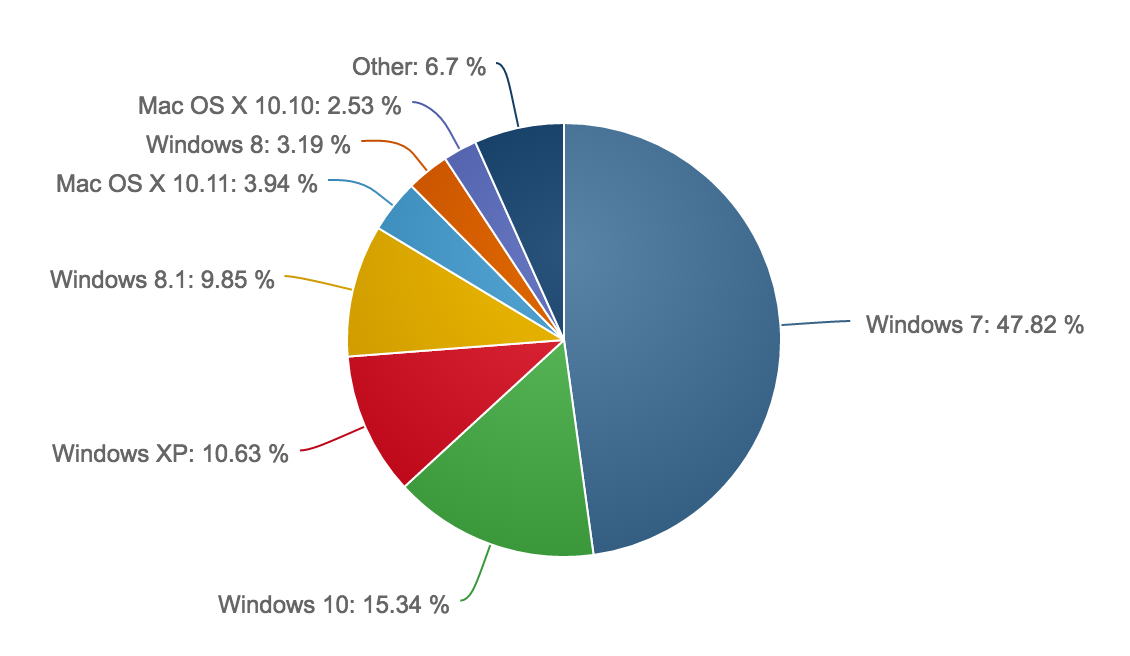
\includegraphics[scale=0.45]{marketshare}
    \caption{Market share reports (January, 2016 to March, 2016)} \label{fig:label}
\end{center}
\end{figure}

\subsubsection{Programming language used for developing}
We are using Arduino, SQLite, Ruby and HTML. We are trying to provide a web service with arduino acting inside the Smart Shoebox. The frontend will be using html and css, while the backend will be using ruby and ruby on rails as a application framework. We thought of using amazon EC2 but if we think of the server as a localhost, we might be using only ruby and ruby on rails for the server with SQLite.

%TABLE2
\begin{table}[H]
\renewcommand{\arrayrulewidth}{1pt}
\renewcommand{\arraystretch}{2.5}
\begin{tabular}
{|p{3.5cm}|p{.5\linewidth}|}\hline

Programming language & Reason\\ \hline
Arduino(hardware) &The main hardware part of our project is based on Arduino. The Smart Shoebox has functions to work provide behavioral motions such as recognizing the temperature and humidity of the shoebox, turning on the fan or infrared lamp as a result of it and so on.
 \\ \hline
MySQL(server side) & We need to have a database to save information about the shoes, users. To easily get and set and manage the information, we have decided to use a database management tool. \\ \hline
Ruby & We first thought of php for the work between the server and web side environment, since we have all learned php in another course. Though we thought it would be much better to learn a new language for this project. Ruby on rails was the interesting programming language in the aspect that it shortens and simplifies the code much more than the php. \\ \hline
HTML5 and CSS3(client side) & We have decided the user interface environment as a web-based structure. The functions of Smart Shoebox will be triggered and managed in the web. \\ \hline

\end{tabular}
\\
\\
\caption{Programming language used for developing}
\label{tab:template}
\end{table}


\subsubsection{Cost estimation (Software / Hardware)}
TABLE III and TABLE IV
%TABLE3
\begin{table}[H]
\renewcommand{\arrayrulewidth}{1pt}
\renewcommand{\arraystretch}{2}
\begin{tabular}
{|p{3.5cm}|p{.5\linewidth}|}\hline

Device & Price (won)\\ \hline
Arduino uno R3 & 7,500\\ \hline
Bread board & 2,400\\ \hline
Wifi module(ESP8266) & 9,000\\ \hline
Temperature Humidity sensor & 3,000\\ \hline
Pressure Sensor & 14,000\\ \hline
Fan(actuator) & 4,000\\ \hline
Board & 2,000\\ \hline
USB cable & 500\\ \hline
jump wire & 2,500\\ \hline
M-F wire & 2,000\\ \hline
Resistance & 200 (5 per unit)\\ \hline
Small LED lamp & 1,000\\ \hline
AA battery & 1,200\\ \hline
transistor & 500 \\ \hline
TOTAL & 49,800 \\ \hline

\end{tabular}
\\
\\
\caption{Cost estimation(Hardware)}
\label{tab:template}
\end{table}

%TABLE4
\begin{table}[h]
\renewcommand{\arrayrulewidth}{1pt}
\renewcommand{\arraystretch}{2}
\begin{tabular}
{|p{3.5cm}|p{.5\linewidth}|}\hline

Software&Task Description\\ \hline
Source Tree(v1.8.3)&Version control \\ \hline
Git(v2.8.1)&Project control\\ \hline
Github&Remote repository\\ \hline
Sublime Text3(3103)&Text editor\\ \hline
mockflow&Wireframe creation\\ \hline
Mac OS X El Capitan&Operating System\\ \hline
Windows 8 / 10&Operating System\\ \hline
Arduino(v1.6.8)&Text editor for Arduino\\ \hline
TOTAL & 0 \\ \hline


\end{tabular}
\\
\\
\caption{Cost estimation(software)}
\label{tab:template}
\end{table}


\subsection{Software in use}
We have researched to find out if there is any existing software or algorithm in use doing a similar task we are trying to provide. We were really surprised to find so much information related to our project. There was a lot of algorithms and systems during the research. The most interesting and related ones were the three below.
\\
\subsubsection{Temperature Humidity Control system}
As anyone can think of the air conditioner or greenhouse there were already a lot of systems and devices doing the actual part of our project to control the temperature and humidity for the given environment. (For our home, or for growing plants in the optimized temperature and humidity, and so on.) Even there were a lot of information about making the Arduino actually work as we planned to.
 %image2
\begin{figure}[H]
\begin{center}
    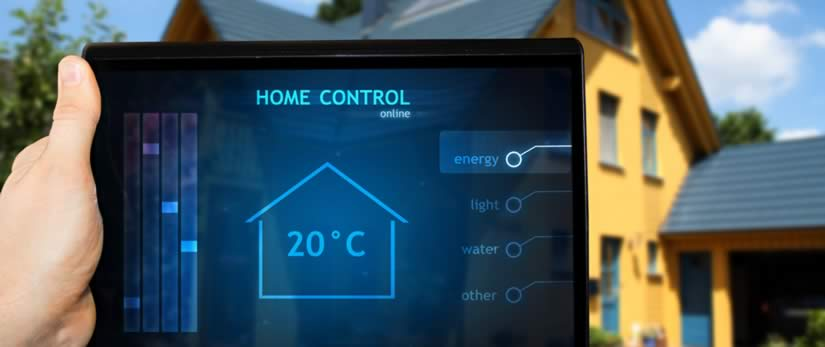
\includegraphics[scale=1.2]{temperature_control}
    \caption{Advance Temperature Control (http://infusionva.com/)} \label{fig:label}
\end{center}
\end{figure}

%image3
\begin{figure}[H]
\begin{center}
    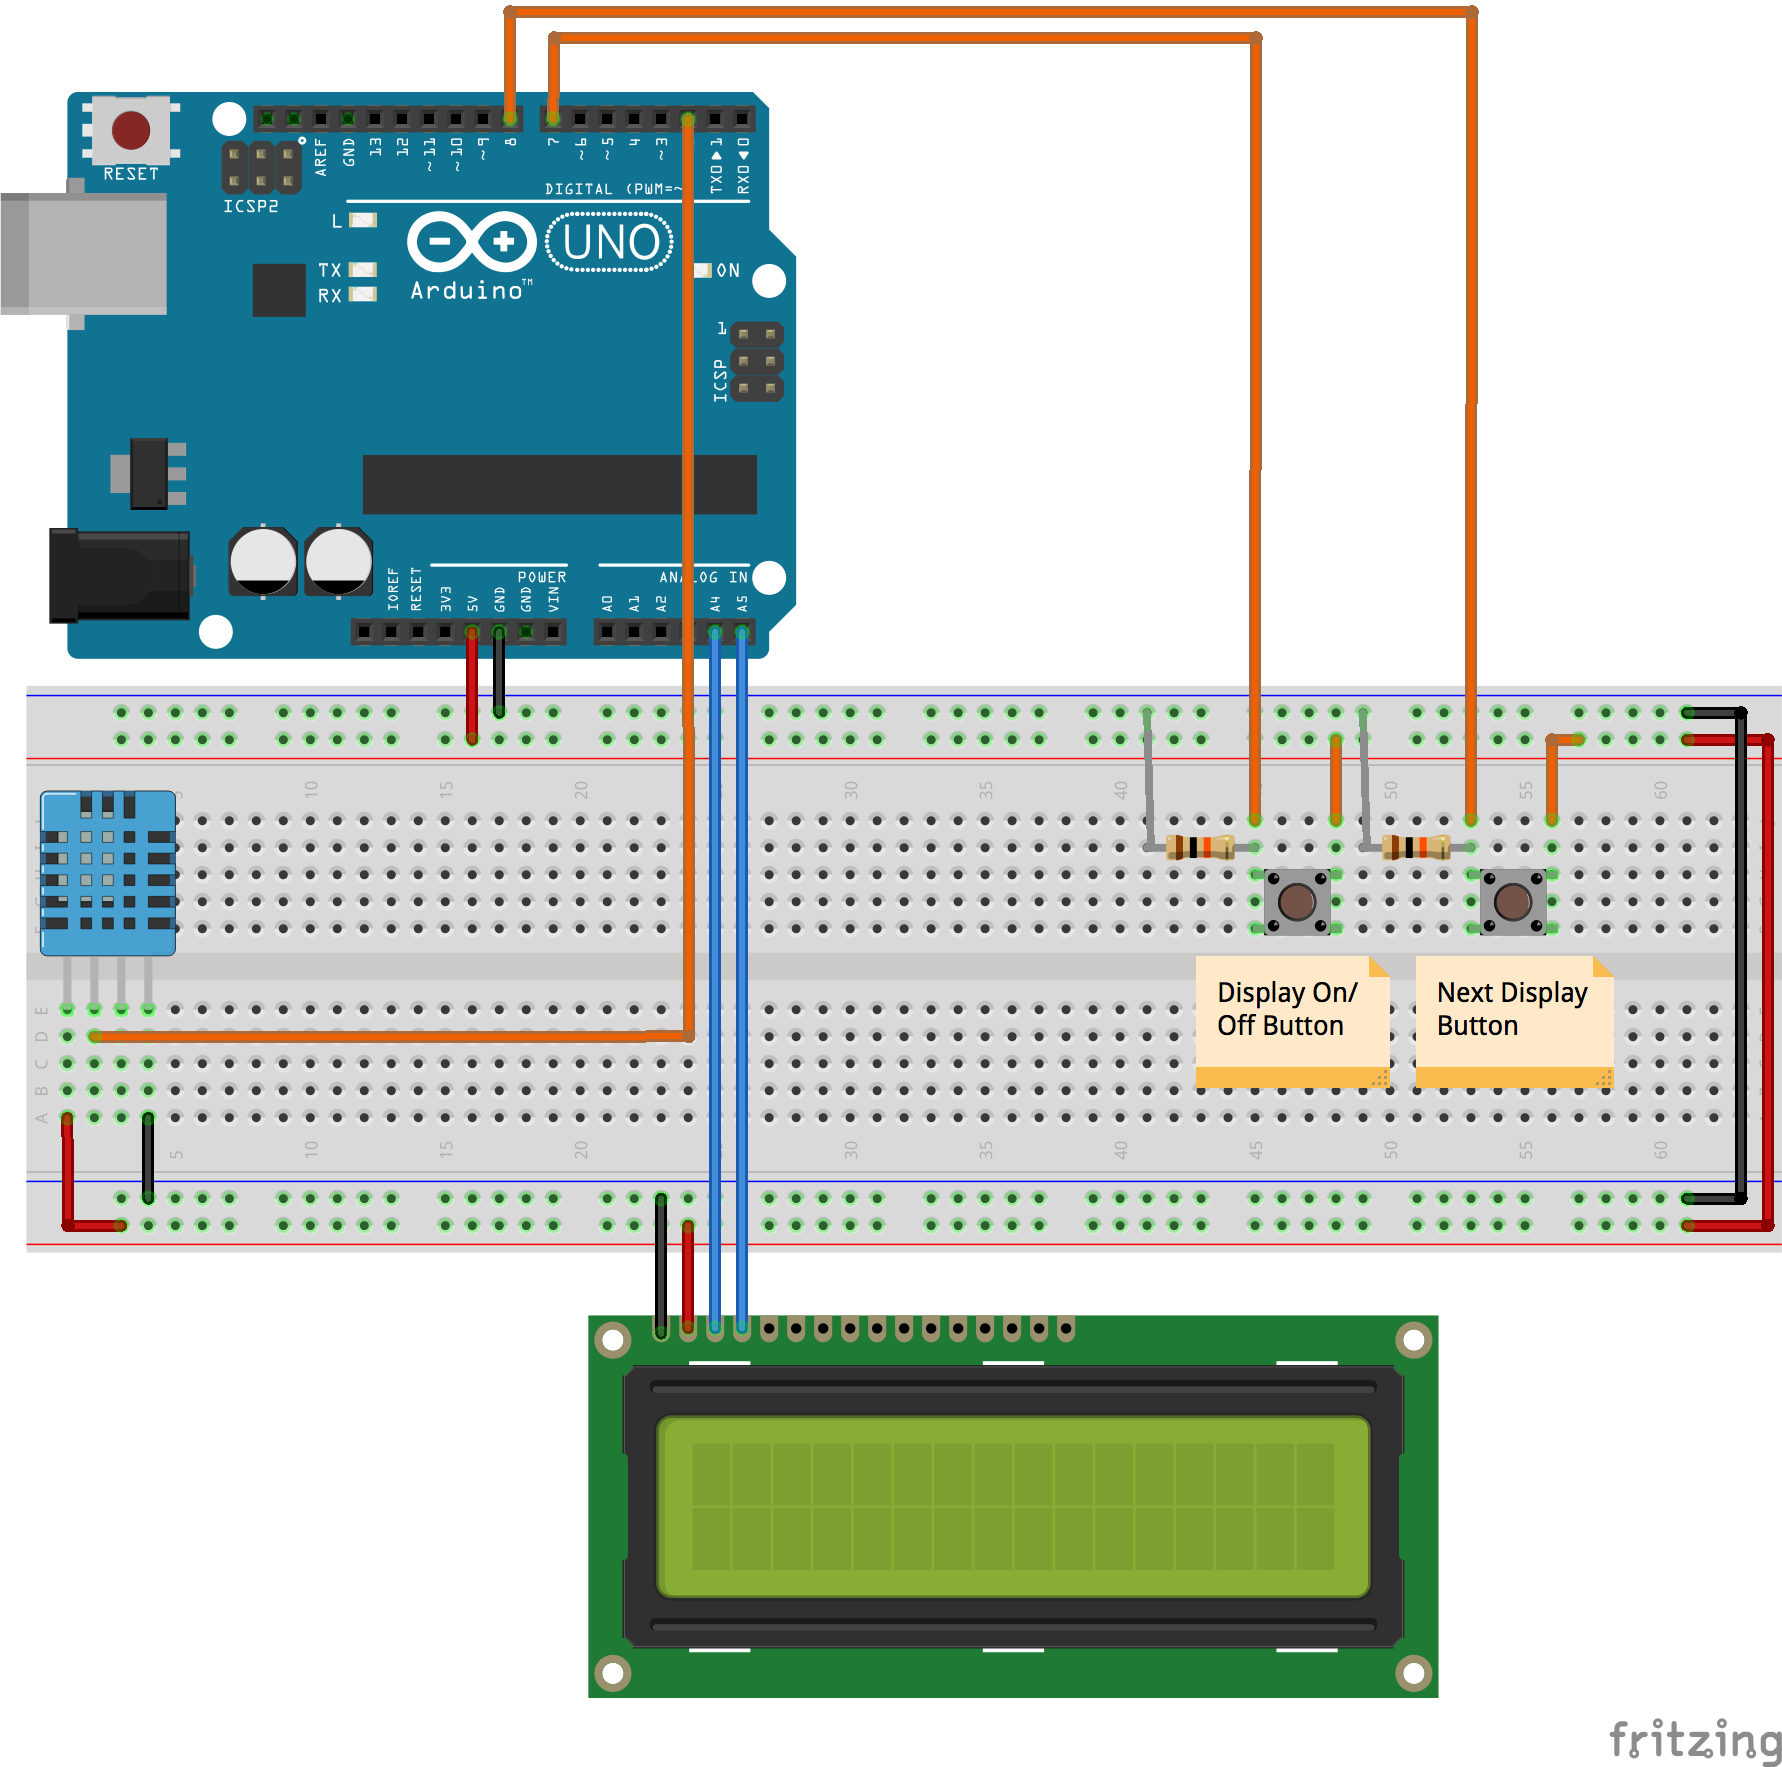
\includegraphics[scale=0.4]{arduino}
    \caption{Airconditioner automatic control through Arduino} \label{fig:label}
\end{center}
\end{figure}


\subsubsection{Recommendation System }
There is an extensive class of Web applications that involve predicting user responses to options. Such a facility is called a recommendation system.
 In Figure above we see an example utility matrix, representing users? ratings of movies on a 1?5 scale, with 5 the highest rating. Blanks represent the situation where the user has not rated the movie. The movie names are HP1, HP2, and HP3 for Harry Potter I, II, and III, TW for Twilight, and SW1, SW2, and SW3 for Star Wars episodes 1, 2, and 3. The users are represented by capital letters A through D.
 The goal of a recommendation system is to predict the blanks in the utility matrix. 
This recommendation system was in common with our project in the point that we will provide a recommendation information for the shoes with the weather APT and color of the shoes matching with the user?s clothes.
%image4
\begin{figure}[H]
\begin{center}
    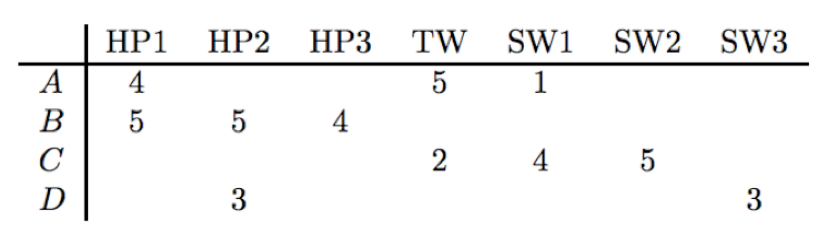
\includegraphics[scale=0.5]{utilitymatrix}
    \caption{utilitymatrix} \label{fig:label}
\end{center}
\end{figure}

\subsubsection{Classification Algorithm in datamining}
Basic Principle (Inductive Learning Hypothesis): Any hypothesis found to approximate the target function well over a sufficiently large set of training examples will also approximate the target function well over other unobserved examples.
%image5
\begin{figure}[H]
\begin{center}
    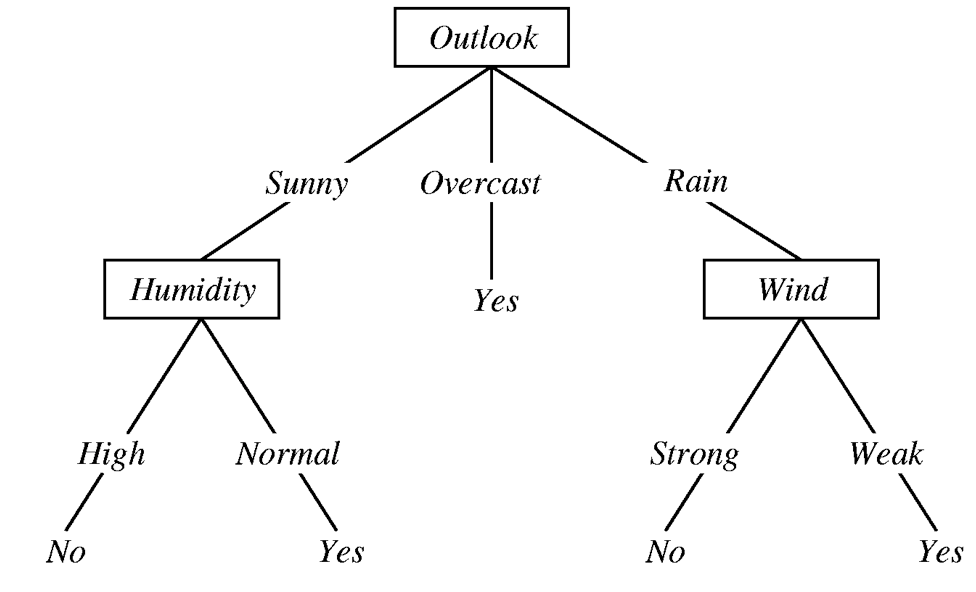
\includegraphics[scale=0.5]{decisiontree_learning}
    \caption{decisiontree learning} \label{fig:label}
\end{center}
\end{figure}

This algorithm was in common with our project in the point that we will classify the shoes. 
\\
\subsubsection{Wifi technology}
The IOT typically employ some kind of embedded technology that allows them to sense conditions such as pressure, humidity, temperature, motion, number of people in an area, etc. And then a technology allows them to connect to other things or the cloud so that they can send the information as well as be programmed. The choice of technology is usually dictated by the physical characteristics of the environment, such as the presence of wood, concrete, metal etc., the density of sensors, desired range, and data rates. Among these technologies, we choice the Wi-Fi as the most successful tool.

Even though there are many ways to communicate wireless, we have decided to use wifi as the communication tool because we also use the website in the base.

Also as we continued the research there were many advantages using the wifi.The most important part was the low cost of wifi. In the semiconductor world, most chips have roughly the same production cost, given some variability in die size and process technology, and with costs falling with increasing volume. While Wi-Fi chips have historically been priced higher than those based on the technologies more often associated with M2M and IoT, manufacturing costs are not necessarily greater. We expect, then, that Wi-Fi chips used in IoT applications and produced in very large numbers will in fact be very cost effective and comparable in price to any other suitable wireless components. And the greater functionality of Wi-Fi (security, power management, robust and mature firmware and drivers, etc.) adds significant value to that cost calculation.

Also the low power gave us the reason to use wifi. IoT applications will seldom require 802.11n and 802.11ac levels of throughput, but lower-cost and more power-friendly solutions based on these (single-stream, for example) will typically be applied and implemented using modern low-power semiconductor process technologies.  Of course, not all IoT applications require battery power, but those that do will see no disadvantage from going the Wi-Fi route as Wi-Fi?s long history of power-saving capabilities applies quite nicely to IoT.
%image5
\begin{figure}[H]
\begin{center}
    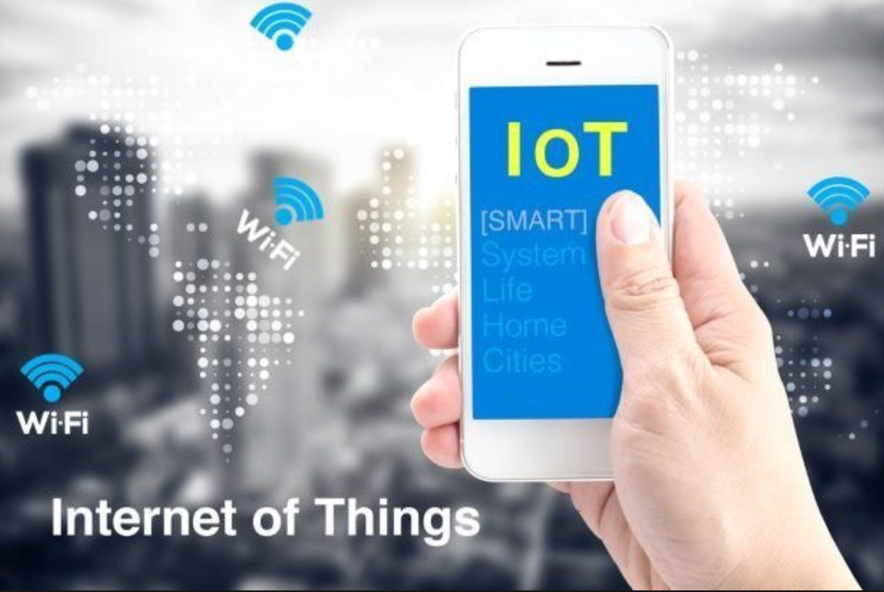
\includegraphics[scale=0.5]{wifi}
    \caption{IoT wifi technology} \label{fig:label}
\end{center}
\end{figure}
\subsubsection{IOT example : Temperature Monitoring}
 Importance of monitoring temperature in industries is quite important as it affects the environment and the process of business e.g. food industry, process industry or any high tech industry such as data centers. Temperature is one of the important parameters which is monitored and controlled to ensure quality output. Most of the high tech industries will have high end climate control systems to monitor and manage temperature, however all organizations cannot afford the luxury of high end systems. Apart from small scale industry, temperature monitoring is important to people with remote cabins, warehouses, or any other location where access to location is difficult.
�
With advancement in software technology and electronics it has become technically feasible to make pocket size high speed and high memory devices. The system is based on the Raspberry Pi which is cost effective and core OS is soft real time OS based on Linux. With Linux as OS, variety of features can be offered such as security, license free usage and community support. The frequency with which data is scanned is customizable and currently programmed to scan every 1 Hr (can be scaled). The data is stored in local MySQL database with updates sent to cloud. The Raspberry Pi also acts as a Server which can be accessed to see logged data. The data in cloud� also represents data graphically and can be downloaded in CSV format.
�
One of the biggest benefits of using Raspberry Pi is the sensor network expansion. The sensors can be added can be configured and further extended with legacy RJ45 cable to and from Sensor Network. Capability to store data from other sensors such as light sensor, humidity, wind sensor, etc. gives flexibility to the system to customize and accommodate quite a lot of wants.

In this IOT example(Temperature Monitoring) we decided to use the ThingSpeak for getting information from Arduino sensor and compatible programming with Raspberry Pi. 
\\
\subsubsection{Selfstarter and Refinery CMS : Ruby on rails web application}

Among funding platforms galore, Self-starter helps you host your own crowdfunding site for your project. Donations are easily made via Amazon Payments, or you can choose your preferred provider. Simple and easy, driven by Ruby on Rails.

Creating a website and managing content is much easier with Refinery CMS. It's a simple modular and extendable content management system. Released in 2009, it's currently undergoing improvements by the community in 10 different languages

From these two open sources, we studied and try to follow the ruby on rails framework for our website. We were really surprised to find a lot of open sources that we can easily find and learn.


\subsubsection{Ruby on rails}
\begin{figure}[H]
\begin{center}
    
\includegraphics[scale=0.5]{ruby}
    \label{fig:label}
\end{center}
\end{figure}
Ruby on Rails, or simply Rails, is a web application framework written in Ruby under the MIT License. Rails is a model?view?controller (MVC) framework, providing default structures for a database, a web service, and web pages. It encourages and facilitates the use of web standards such as JSON or XML for data transfer, and HTML, CSS and JavaScript for display and user interfacing. In addition to MVC, Rails emphasizes the use of other well-known software engineering patterns and paradigms, including convention over configuration (CoC), don't repeat yourself (DRY), and the active record pattern.
\subsubsection{Database Management System}

A database is an organized collection of data. It is the collection of schemas, tables, queries, reports, views and other objects. The data are typically organized to model aspects of reality in a way that supports processes requiring information, such as modelling the availability of rooms in hotels in a way that supports finding a hotel with vacancies.

A database management system (DBMS) is a computer software application that interacts with the user, other applications, and the database itself to capture and analyze data. A general-purpose DBMS is designed to allow the definition, creation, querying, update, and administration of databases. Well-known DBMSs include MySQL, PostgreSQL, Microsoft SQL Server, Oracle, Sybase, SAP HANA, and IBM DB2. A database is not generally portable across different DBMSs, but different DBMS can interoperate by using standards such as SQL and ODBC or JDBC to allow a single application to work with more than one DBMS. Database management systems are often classified according to the database model that they support; the most popular database systems since the 1980s have all supported the relational model as represented by the SQL language.

We have decided to use the database to store information about the users and the shoes inside the Smart Shoebox. With the stored information we can realize the feature of managing all the shoes the user possess.
\begin{figure}[H]
\begin{center}
    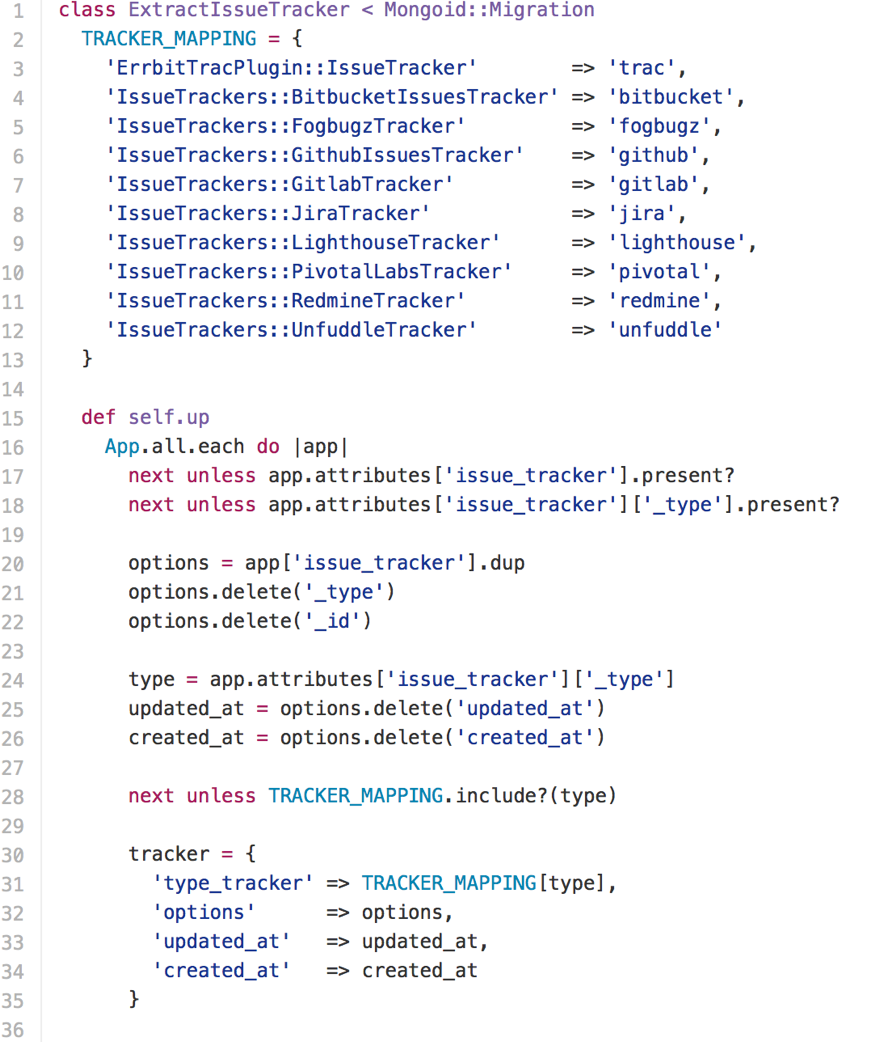
\includegraphics[scale=0.55]{database}
    \caption{Example for database in ruby on rails}\label{fig:label}
    This is the open source we have researched to study the database inside ruby on rails.
\end{center}
\end{figure}
\subsection{Task Distribution}
We have decided to distribute the project in big parts to make each participants to be responsible for the assigned parts. Still every person has to know how the project is going on in a big picture while being responsible for the assigned part.
%TABLE5
\begin{table}[H]
\renewcommand{\arrayrulewidth}{1pt}
\renewcommand{\arraystretch}{2.5}
\begin{tabular}
{|p{4cm}|p{4cm}|}\hline
Name & Responsible Part\\ \hline
Kwon GyuHyeok&Arduino programming\\ \hline
Shin MinKi&SQLite, database schema\\ \hline
Kim JungHyun&Ruby on rails, Wireless fidelity control\\ \hline
Ko ByungHee&Ruby on rails, Bootstrap\\ \hline
\end{tabular}
\\
\\
\caption{Task Distribution}
\label{tab:template}
\end{table}

% 4. specification
\section{Specification}
The specification is mostly in pseudocode and additionally graphs and charts will be used to specify the requirements. Particularly, mockflow will be used to wireframe the user interface. The pseudocode is a little bit close to the programming languages we have already learned during other courses while disregarding the details of the grammar.
\subsection{Optimization function}
\subsubsection{Temperature/Humidity control through electric fan (automatic)}
\subsubsection{Temperature/Humidity control through ultraviolet lamp (automatic)}
The arduino sensor receives temperature and humidity as inputs and truns on fan and ultraviolet lamp when temperature drops below 15 Celsius degree or humidity is higher than 

\subsubsection{Drying feature (on demand)}
In case the user?s shoes get wet by rain or other liquids the user can request for drying function. The function will turn on fan on maximum rate and intensity of lamp will be middle.
\subsubsection{Sterilization function (on demand)}
In case the user feels the need for sterilization, user can request for this function. The function will turn on fan on middle rate and intensity of lamp will be maximum.
\subsubsection{Deodorization function (on demand)}
In case the user feels the need for deodorization, user can request for this function, which triggers a deodorant to shoot out. The Arduino will trigger the deodorant.
\subsubsection{Deodorization function (automatic)}
This function will provide the Smart Shoebox to trigger the deodorant to shoot out in one hour interval. 

\subsubsection{Intensity control feature}
The user can choose the intensity level of fan and lamp. Intensity is calculated as number between 1 to 3, which means maximum, middle, minimum.

\subsection{Management function}
This management function is mostly about modeling and categorizing the shoes. Through the serial number scanning, captured image, 3D scanning and user input, the information about the user and shoes are managed in the database. 
\subsubsection{Shoe categorization function (bar-code scanning)}
\subsubsection{Shoe categorization function (user input based)}
\subsubsection{Shoe categorization function (captured image)}
\subsubsection{Shoe categorization function (3D scanning)}
\subsubsection{Setting the proper management tool}Modeling

The big arrow pointing to the database will be one of the ways of receiving the information of the shoes by the user. Like we mentioned at above part the ways will be the serial number scanning, analyzing the captured image, 3D scanning and analyzing user input.

%image6
\begin{figure}[H]
\begin{center}
    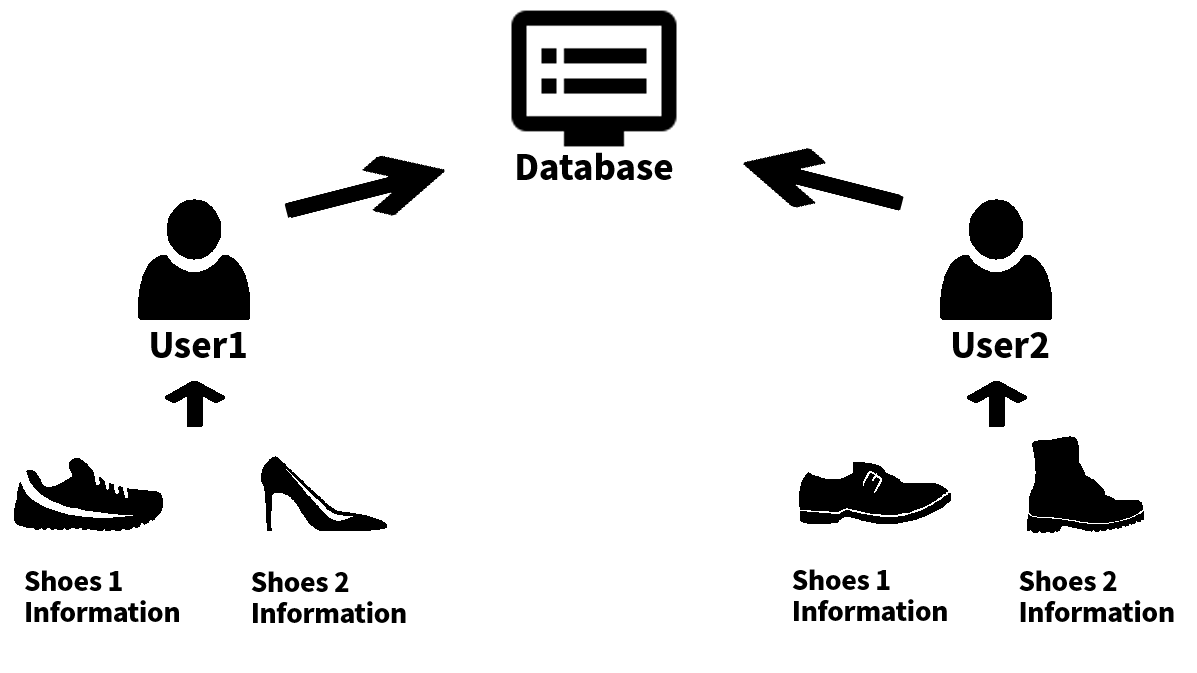
\includegraphics[scale=0.28]{management1}
    \caption{Shoe information into the database} \label{fig:label}
\end{center}
\end{figure}
%image7
\begin{figure}[H]
\begin{center}
    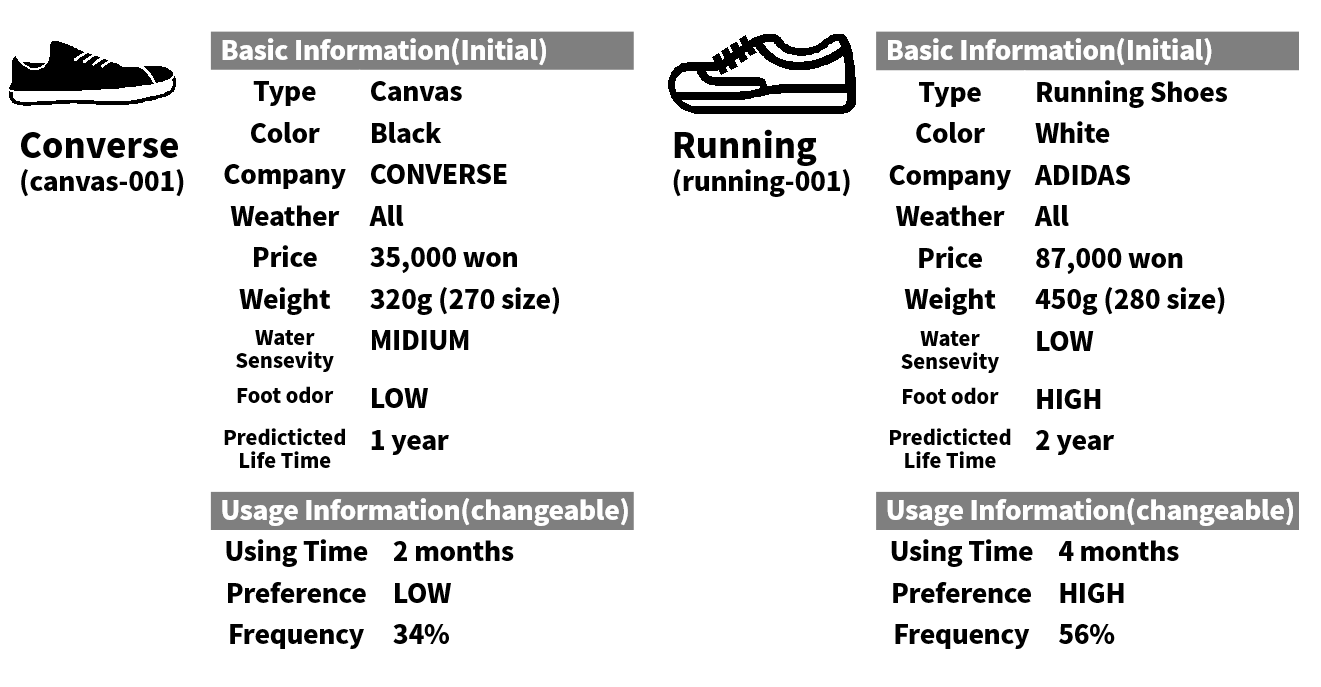
\includegraphics[scale=0.24]{management2}
    \caption{Example of the shoes modeling } \label{fig:label}
\end{center}
\end{figure}

As we can see in Fig.7 the saved information of the shoes will be assigned to each model we will provide before. For each model the proper care solution will be provided. 
The modeling of each shoe into a number of category and setting the proper care solution will be the most important part to realize this function. Also at the same time it is the most ambiguous part before the design phase.



\subsection{Analysis function}
\subsubsection{Absence of shoes analysis (Base information)}
We have decided to analyze the absence of shoes by weight sensor and use it as a base information for other analysis functions. The absence timer will be on and count the time of the shoes absence.

\subsubsection{Durability analysis}
Durability is set to decrease by the time the shoe has been put on increases. We have decided the average shoes usage time as 12 hours a day and the durability changes while the absence time increases. Less than 2 weeks is considered to be a new one. Between 2 weeks and 4 weeks is considered to be not bad. 
Between 4 weeks and 8 weeks is considered to be washed. Between 8 weeks and 16 weeks is considered to be careful. More than 16 weeks the shoes is considered to be replaced.

\subsubsection{Life prediction analysis}
Based on the information of absence time, we provide the expected  life of the shoes. We subtract the absence time from the original life time.

\subsubsection{Preference analysis (personal)}
\subsubsection{Preference analysis (general)}
Based on the information of absence time for a number of users, we provide the preference information of the shoes in general aspect. Since we all store the information about the shoes of the user in the database this is possible in both personal and general aspect. Using this Big data, the user can know which shoes are popular nowadays.

\subsubsection{Frequency analysis}
Based on the information of absence time, we provide the frequency information for the shoes in percentage. We devide the used days by the whole day since the user started to use the Smart Shoebox.



\subsection{Recommendation function}
Smart Shoes cabinet will provide recommendation information with percentages based on different kind of aspects. Of course the final choice is up to the user. The main recommendation standard is the weather. So we have decided to place a screen for the weather.
%image8
\begin{figure}[H]
\begin{center}
    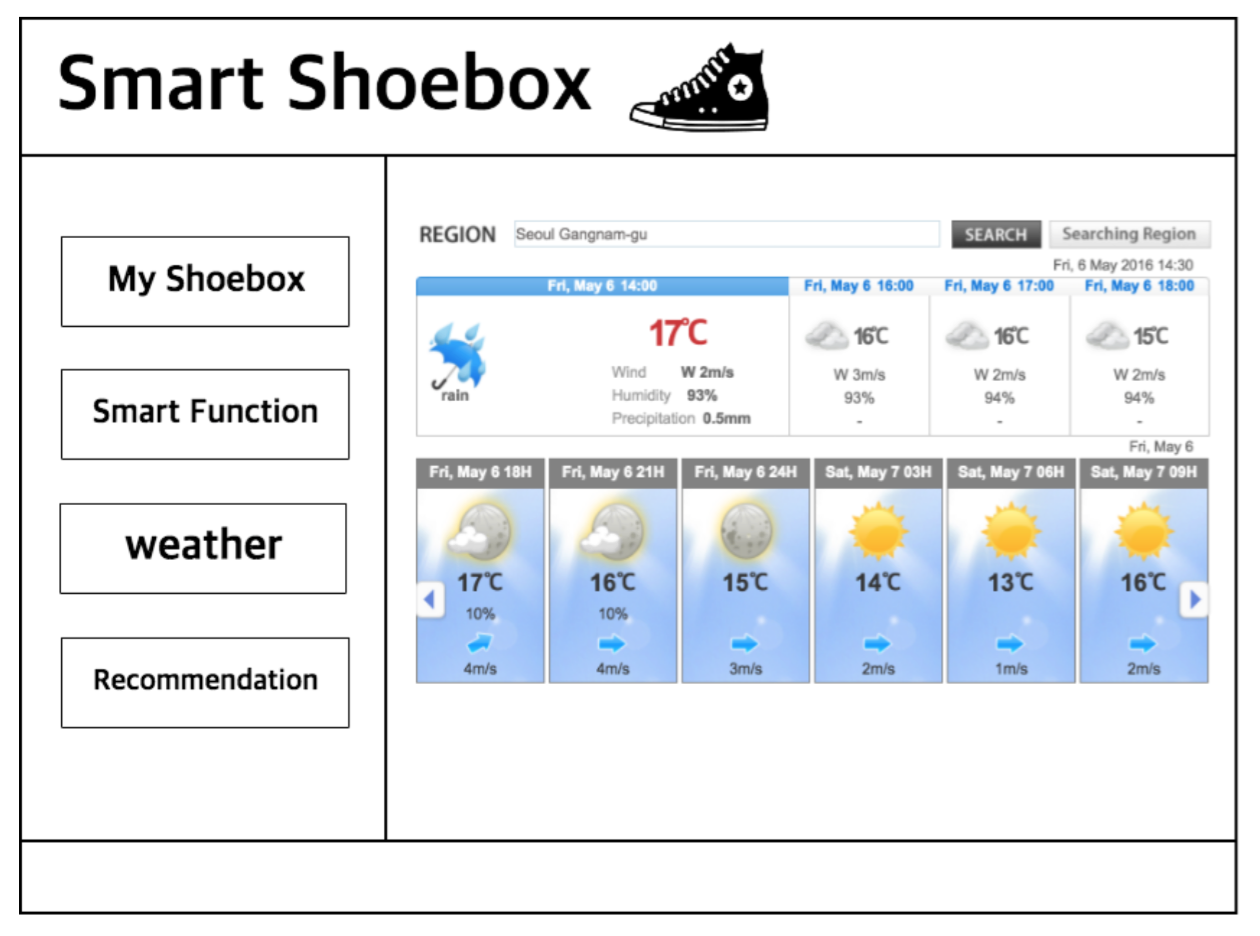
\includegraphics[scale=0.4]{UI1}
   \caption{Weather on the web screen}\label{fig:label}
\end{center}
\end{figure}
%image9
\begin{figure}[H]
\begin{center}
    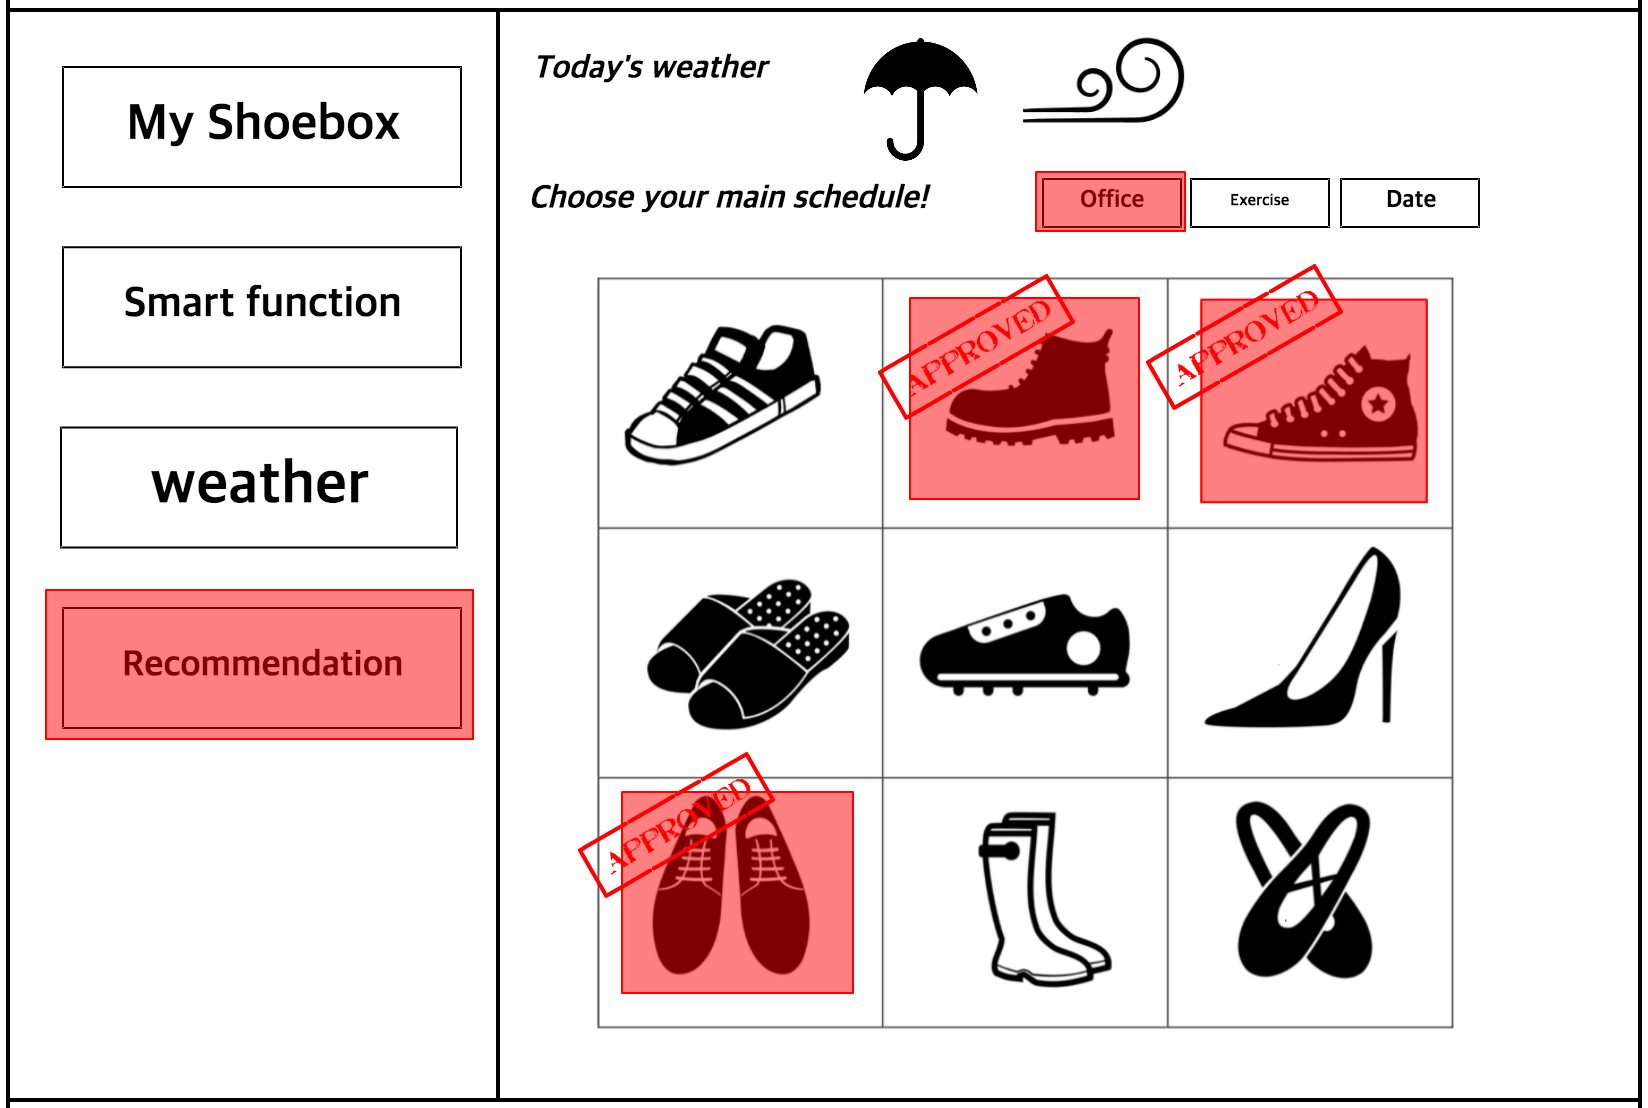
\includegraphics[scale=0.29]{UI2}
   \caption{Recommendation on the web screen}\label{fig:label}
\end{center}
\end{figure}
\subsubsection{Recommendation based on weather forecast }
With weather API, the proper type of shoes is recommended. We decided to classify weather in three cases. ('Sunny' and 'Cloudy' and 'Rainy or Snowy') We will restrict the recommendation choices by the weather becomes bad. The word proper (the proper shoes for the weather) will be represented in the shoes modeled information in the database.

\subsubsection{ Recommendation based on the use of shoes}
Recommending the proper shoes type which matches with the user?s activity. The word proper (the proper shoes for the activity of the user) will be represented in the shoes modeled information in the database.

\subsubsection{Recommendation based on the color of shoes}
Recommending the proper shoes color which balances with the users clothing color. The word proper (the proper shoes for the clothes of the user) will be represented in the shoes modeled information in the database.

\subsubsection{ Notice of recommendation rate by color}
\subsubsection{Notice of recommendation rate by percentage}
Showing the recommendation rate by different colors. For example, if the shoes are recommended, a specific color will appear on the shoe rack or on the screen the user is looking at. 
Showing the recommendation rate by percentage. If the shoes are recommended strongly, the percentage will appear on the shoe rack or on the screen the user is looking at. 



\subsection{Notification function}
\subsubsection{Recognition of contamination by sensor}
\subsubsection{Notification for contamination by message}
With the increased weight, notification is given for contamination. The weight to be sensed is defined to be 20g.
After the recognition of contamination, the information is notified to the user through messages on the screen.


\subsection{Networking / Remote control function (UI)}
\subsubsection{Control function through web programming (main)}
\subsubsection{Control function through mobile (sub)}
\subsubsection{Control function through embedded system (sub)}
To realize this function we will provide a user interface through mainly web and additionally mobile and a screen for the Smart Shoebox. The already mentioned functions before will be on the UI so that the user can interact with the system. The temperature and humidity will be provided on the screen the user will be seeing. Optimaization function, management function, analysis function, recommendation function, notification function will be on the main screen for users to be able to use. 

%image10
\begin{figure}[H]
\begin{center}
    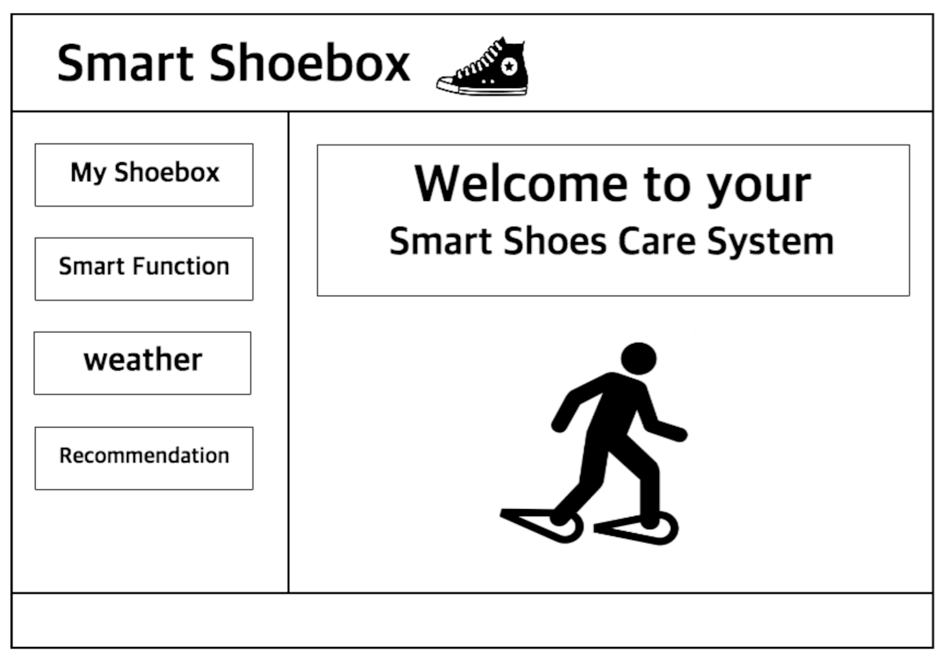
\includegraphics[scale=0.5]{UI4}
   \caption{Main page for Smart Shoebox}\label{fig:label}
\end{center}
\end{figure}
%image11
\begin{figure}[H]
\begin{center}
    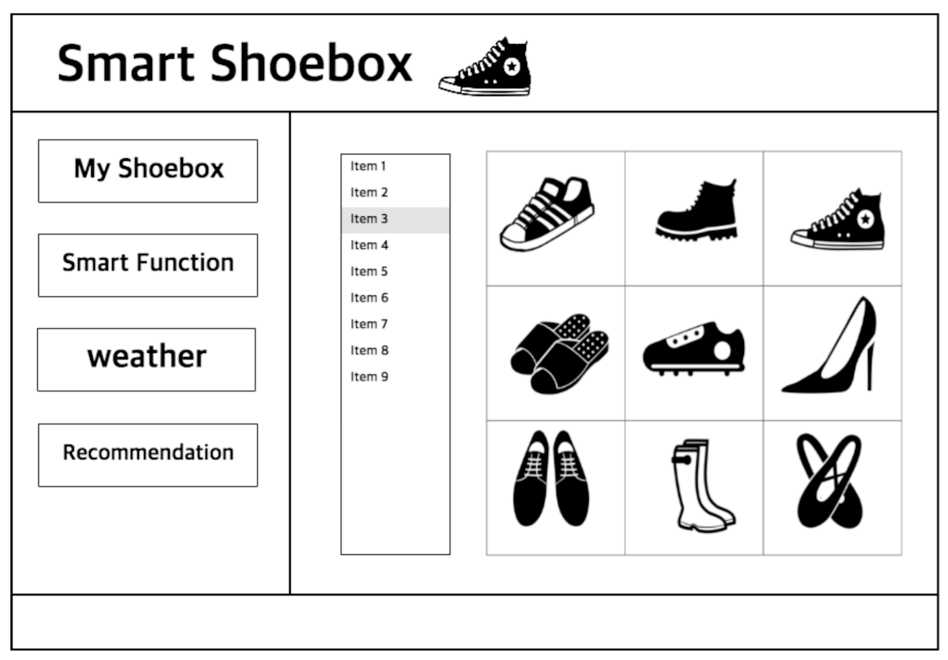
\includegraphics[scale=0.5]{UI5}
   \caption{Shoes status for Smart Shoebox}\label{fig:label}
\end{center}
\end{figure}


% 5. Architecture Design and Implementation
\section{Architecture Design and Implementation}
\subsection{Overall architecture} We have three modules consisting of the Smart shoebox. First part is the Arduino module, which receives the request of the user by jQuery and reacts. It also provides temperature, humidity, pressure information to the web server, which is provided by the sensor of the Arduino. The second and third part is a set of web service. One is the front end module(HTML/CSS) and the other is the back end module(SQLite). The front end is mainly reacting with the client(user) and back end is mainly reacting with the server. The user can add a new item and sign up to the Smart Shoebox service. The server will provide the detail information of the registered item and recommend. As you can see in Fig. 12 all modules interact with each other. 
%image12
\begin{figure}[H]
\begin{center}
    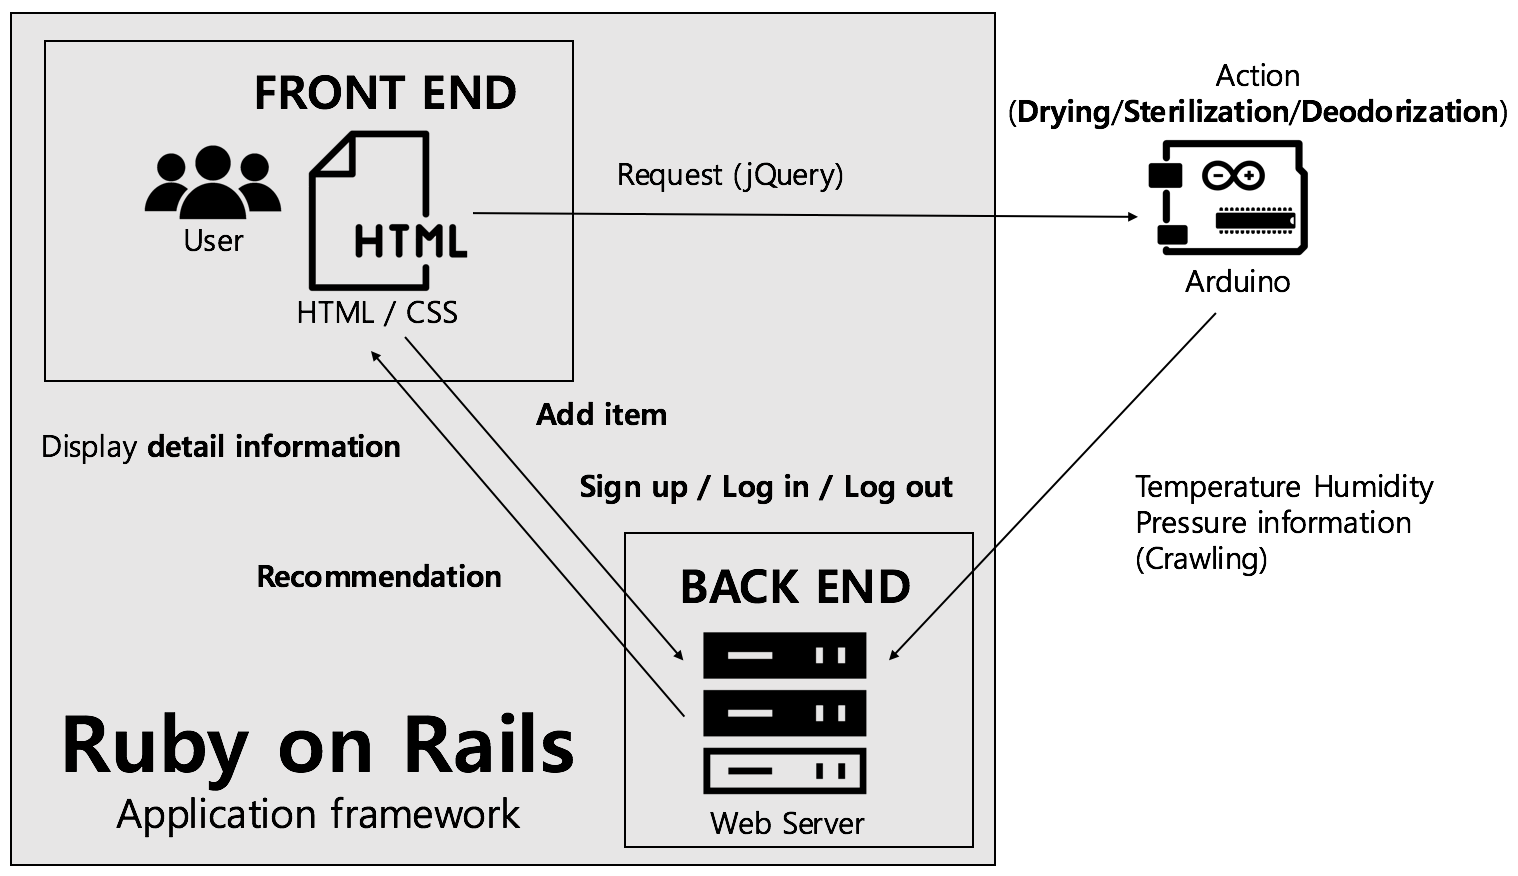
\includegraphics[scale=0.32]{overallarchitecture}
   \caption{Overall system architecture}\label{fig:label}
\end{center}
\end{figure}
\subsection{Directory organization}
We have three big folders, which follows the overall system architecture. One is the arduino and another is website folder for the ruby on rails and the last one is a folder for the LaTex documentaion.
\begin{figure}[H]
\begin{center}
    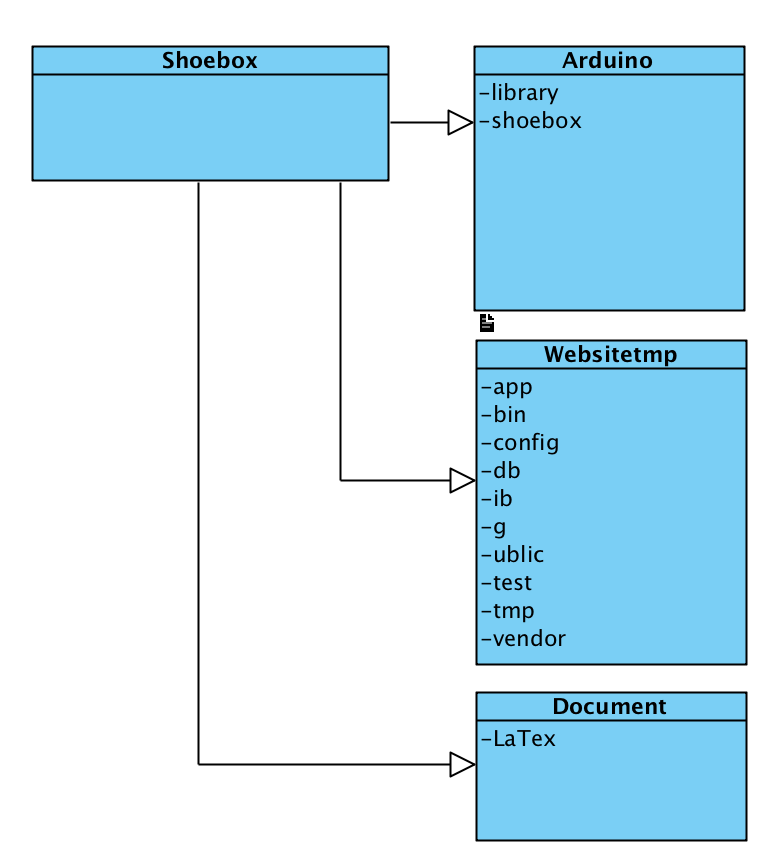
\includegraphics[scale=0.65]{directory1}
   \caption{Directory organization}\label{fig:label}
   This is the directory organization using UML. There are three big parts including Arduino, Website and Document.
\end{center}
\end{figure}

%TABLE6

\begin{table}[H]
\renewcommand{\arrayrulewidth}{1pt}
\renewcommand{\arraystretch}{2}
\begin{tabular}
{|m{3cm}|m{2.2cm}|m{2.2cm}|}\hline

Directory & File names & Module name\\ \hline
/project/arduino/library & dht11.cpp, dht11.h & arduino\\ \hline
/project/arduino/shoebox & shoebox.ino & arduino\\ \hline
website/app/controller & application-controller.rb, home-controller.rb, mybox-controller.rb, smart-controller.rb & rails model\\ \hline
/project/website/app/helper & application-helper.rb, home-helper.rb, mybox-helper.rb, smart-helper.rb & rails helper\\ \hline
/project/website/app/models & shoe.rb, user.rb & rails model\\ \hline
/project/website/app/views & ... & rails view\\ \hline
/views/home & index.html.erb & rails view\\ \hline
/views/layouts & application.html.erb & rails view\\ \hline
/views/mybox & information.html.erb, detail.html.erb, new.html.erb & rails view\\ \hline
/views/smart & index.html.erb & rails view\\ \hline
/project/website/bin & bundle, rails, rake, setup & rails bin\\ \hline
/project/website/config & routes.rb & rails routes\\ \hline
/project/website/db & schema.rb,seeds.rb & rails db\\ \hline
/project/website/db/migrate & 20160525053629-devise-create-users.rb, 20160525053708-create-shoes.rb & rails db migrate\\ \hline
/project/website/lib & & rails lib\\ \hline
/project/website/log & development.log & rails log\\ \hline
/project/website/public & 404.html, 422.html, 500.html & rails public\\ \hline
/project/document/LaTex & document.tex, document.aux, document.log, document.pdf & documentation\\ \hline


\end{tabular}
\\
\\
\caption{directory organization}
\label{tab:template}
\end{table}

\subsection{Module1:Arduino}
%image13
\begin{figure}[H]
\begin{center}
    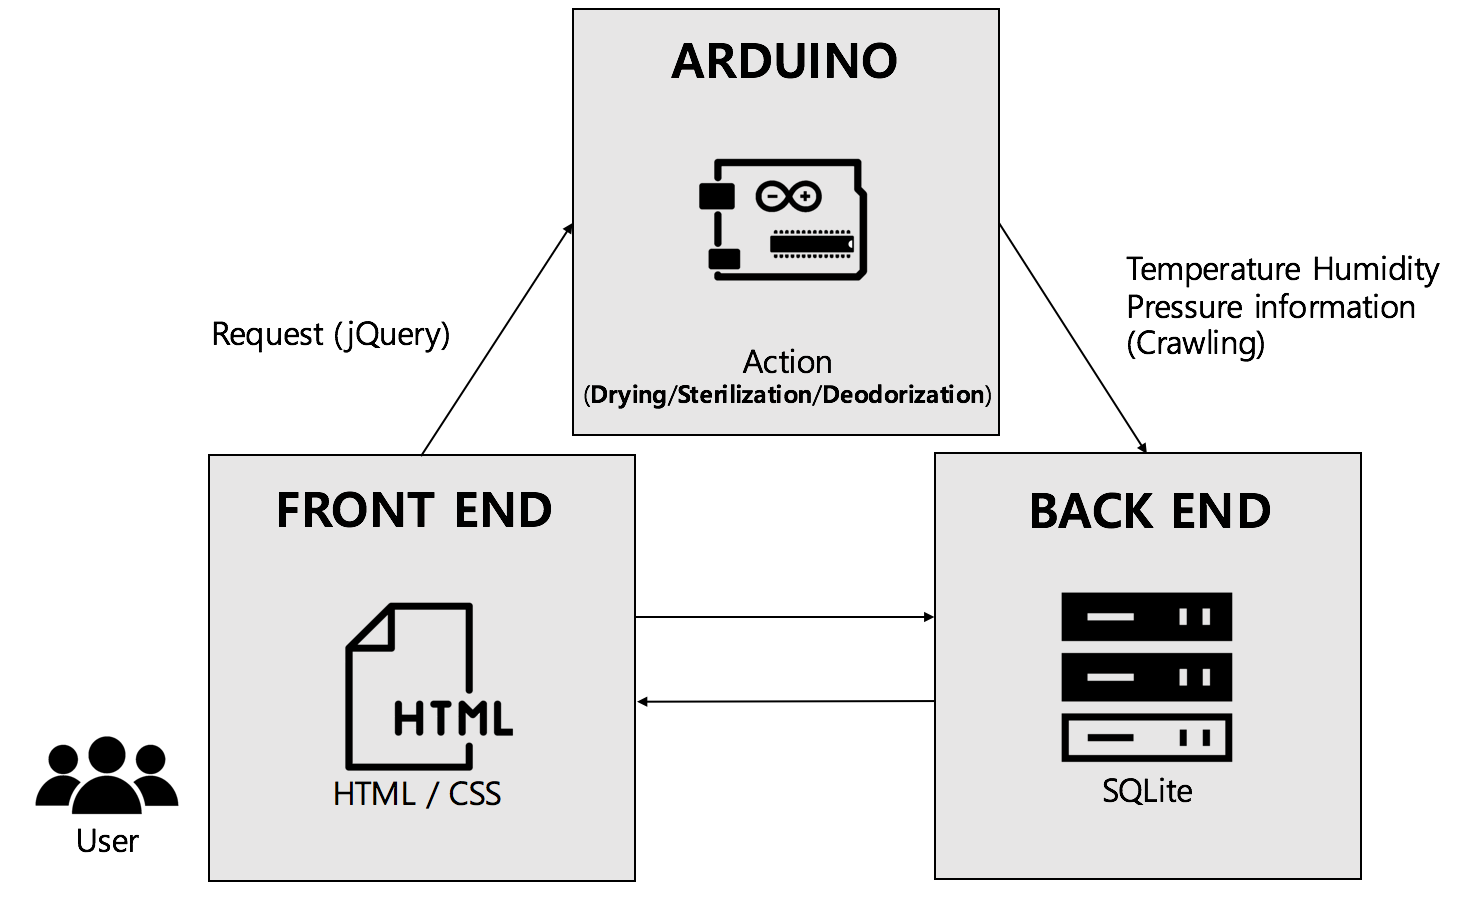
\includegraphics[scale=0.35]{module1}
    \caption{Module1 : Arduino} \label{fig:label}
\end{center}
\end{figure}
\begin{figure}[H]
\begin{center}
    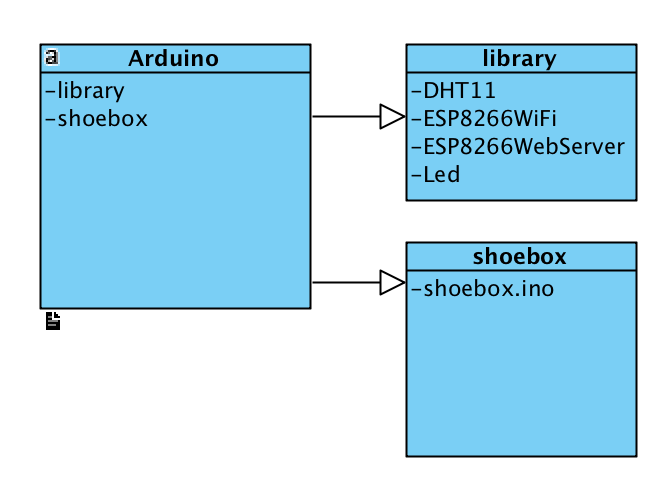
\includegraphics[scale=0.7]{directory2}
   \caption{Arduino : Directory organization}\label{fig:label}
\end{center}
\end{figure}
\subsubsection{Purpose} First, we are trying to receive information about the temperature, humidity, and pressure by each related sensors. The pressure sensor is for the recognition of the shoes. Second, we are trying to perform the smart functions the user will be requesting. Third, we are trying to interact with the Smart Shoebox with wifi module of Arduino.
\subsubsection{Functionality} The functionality fits to the purpose of the module. It provides wirless communication between the Smart Shoebox and the user interacting with the website. Also the additional sensors can measure the temperature, humidity and pressure. Consequently with the informations of the sensor the fan, infrared lamp and deodorant will carry out the smart functions we designed.
\subsubsection{Location of Source Code}/project/shoebox/arduino
\subsubsection{Class component}There are three components in the Arduino class.
\\
- Setup( ) : This is the work done only at the first time when the Arduino starts to activate. 
(For example, setting up the rate or the wifi module.)
\begin{figure}[H]
\begin{center}
    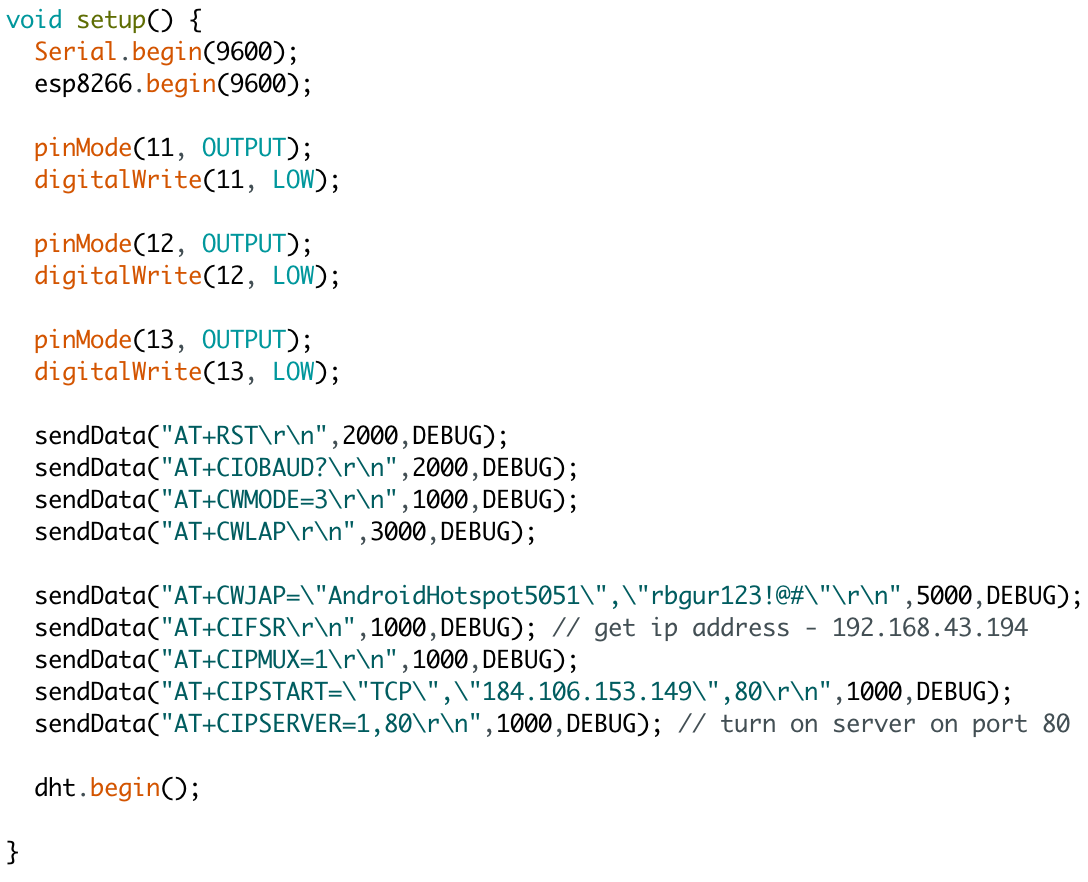
\includegraphics[scale=0.44]{setup}
  \label{fig:label}
\end{center}
\end{figure}
- Loop( ) : This is the ongoing work of Arduino, while the Smart Shoebox is on. It is repeatedli reading the temperature and humidity from the sensor.
\begin{figure}[H]
\begin{center}
    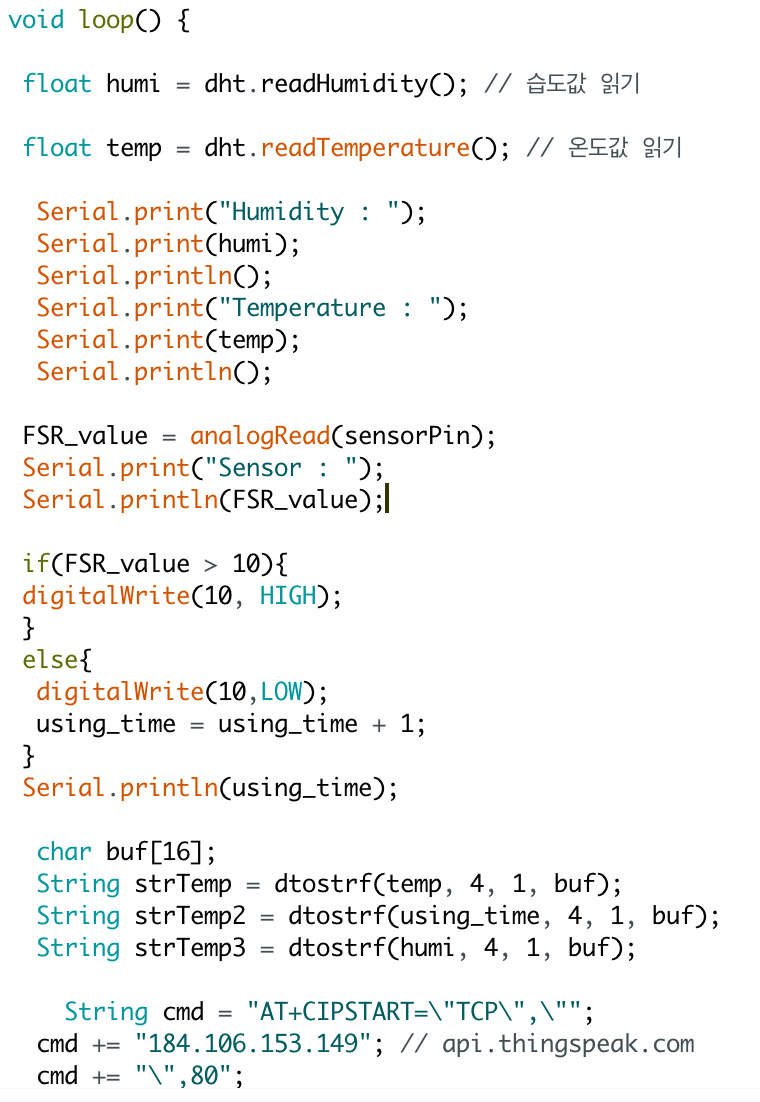
\includegraphics[scale=0.55]{loop}
  \label{fig:label}
\end{center}
\end{figure}
- Library : The open source provided to help developing Arduino.
\subsubsection{Where it is taken from} It is taken from the library list of Arduino official homepage. Arduino Playground is a wiki where all the users of Arduino can contribute and benefit from their collective research.

(http://playground.arduino.cc/Main/LibraryList)
\subsubsection{How and Why we use it}We connect all the modules, sensors, LED light bulbs, fan and infrared lamp to the Arduino Uno, the main board. Additionally, with the libraries provided, we write down the code for the the functions and compile. When the codes are uploaded to the main board, the required functions are performed.\\

\subsection{Module2:Ruby on Rails}
%image14
\begin{figure}[H]
\begin{center}
    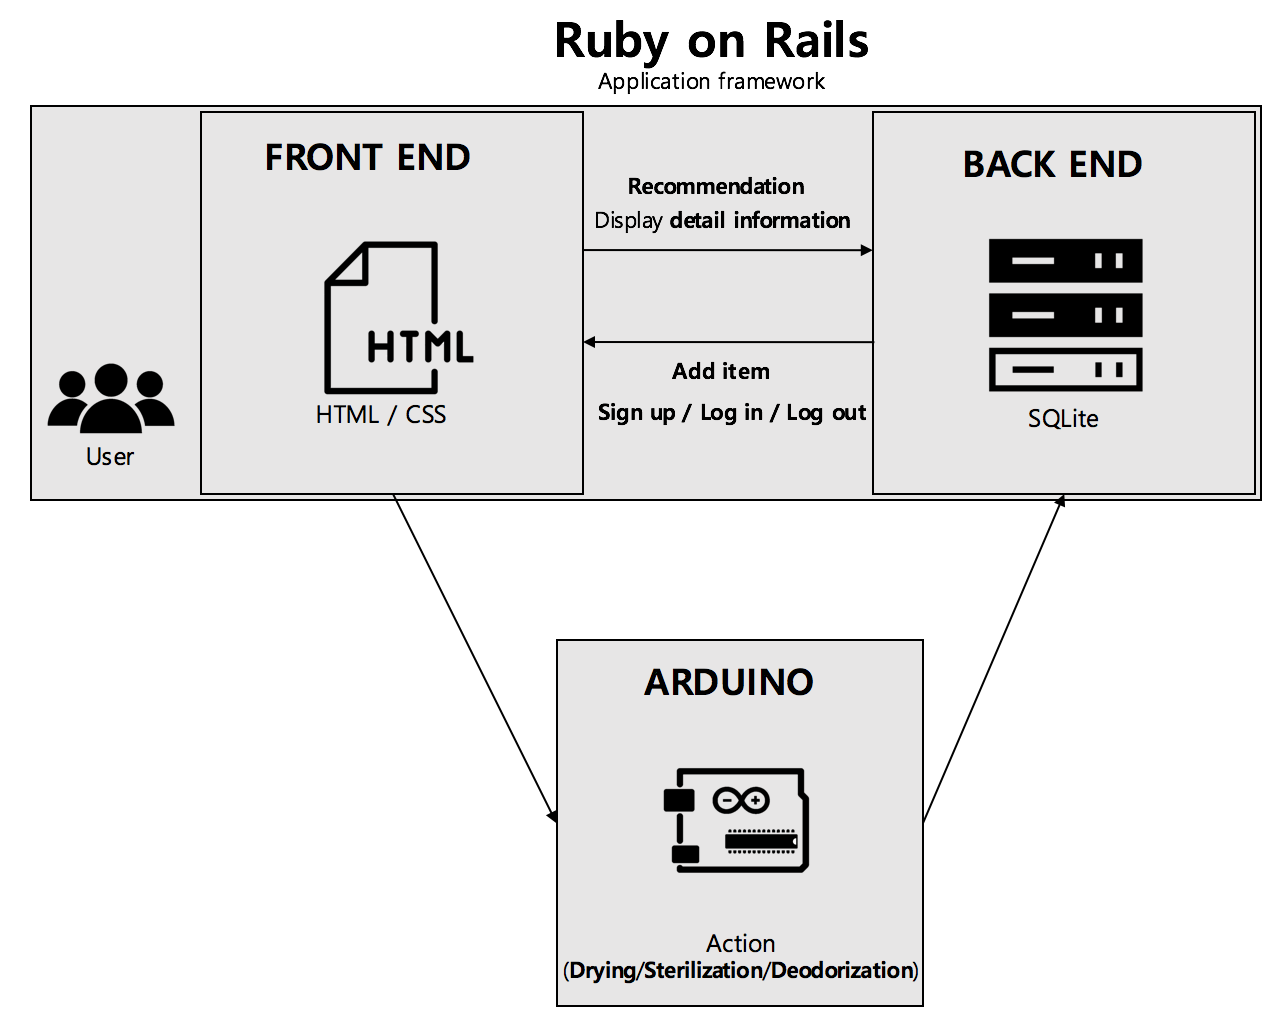
\includegraphics[scale=0.38]{module2}
    \caption{Module2 : Ruby on Rails} \label{fig:label}
\end{center}
\end{figure}
\begin{figure}[H]
\begin{center}
    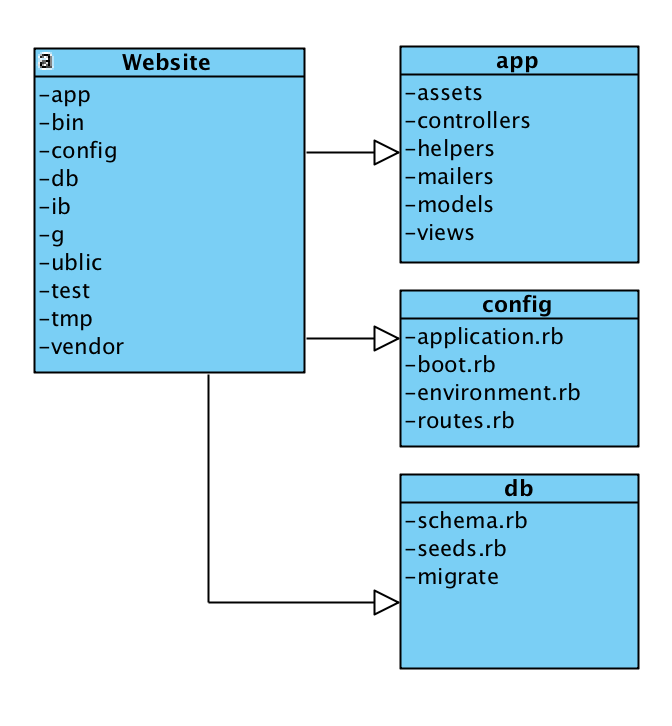
\includegraphics[scale=0.58]{rubyonrails}
  \caption{Ruby on Rails : Directory organization}\label{fig:label}
\end{center}
\end{figure}
\begin{figure}[H]
\begin{center}
    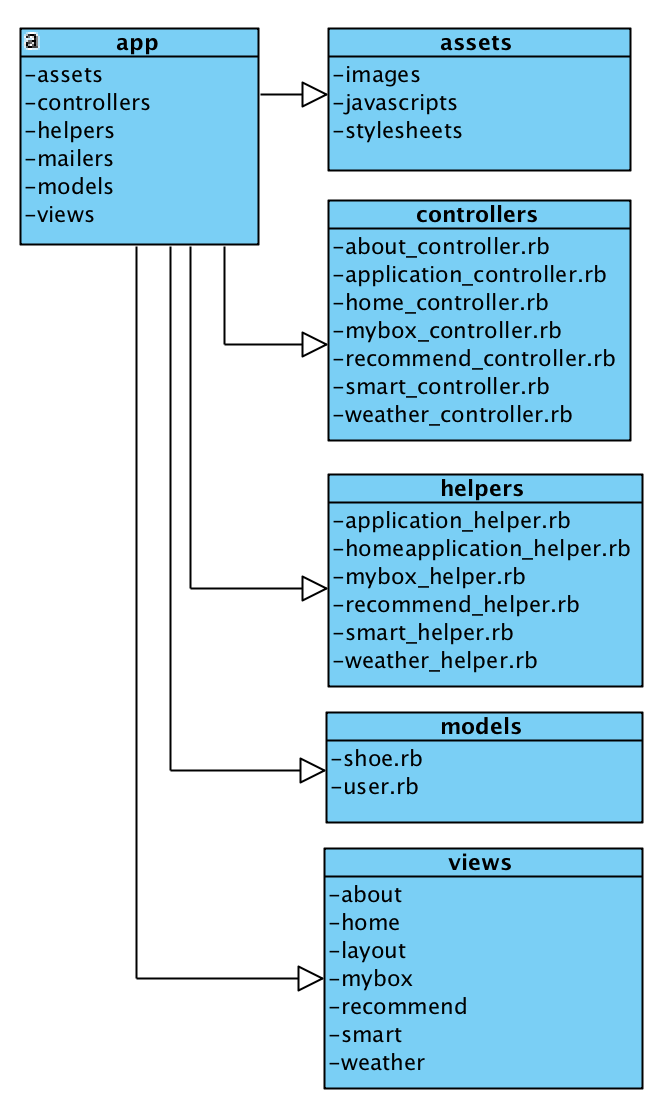
\includegraphics[scale=0.65]{app}
  \caption{Ruby on Rails : app : Directory organization}\label{fig:label}
\end{center}
\end{figure}
\begin{figure}[H]
\begin{center}
    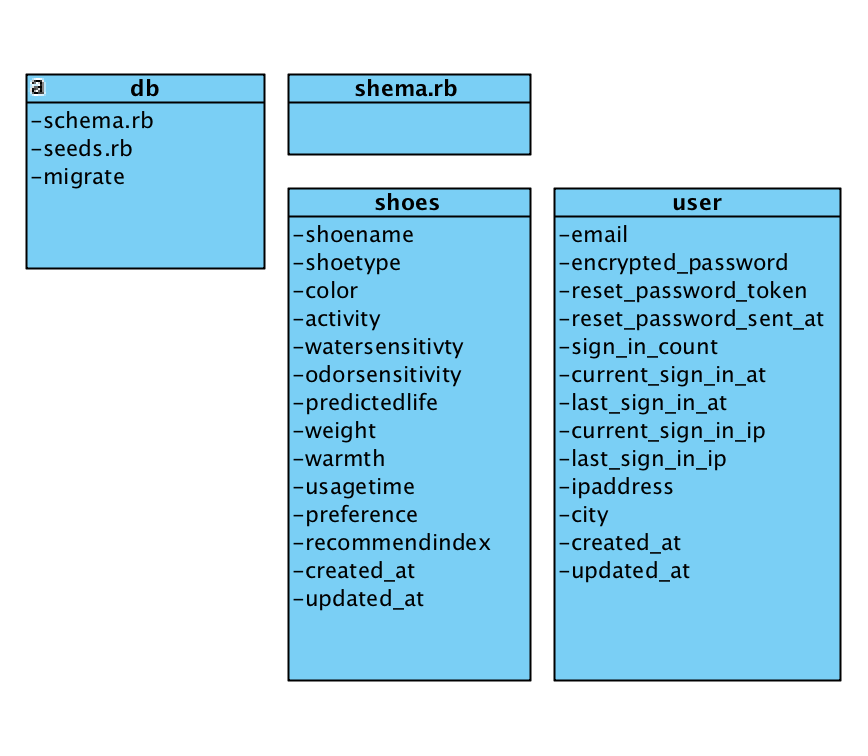
\includegraphics[scale=0.55]{db}
  \caption{Ruby on Rails : db : Directory organization}\label{fig:label}
\end{center}
\end{figure}
\begin{figure}[H]
\begin{center}
    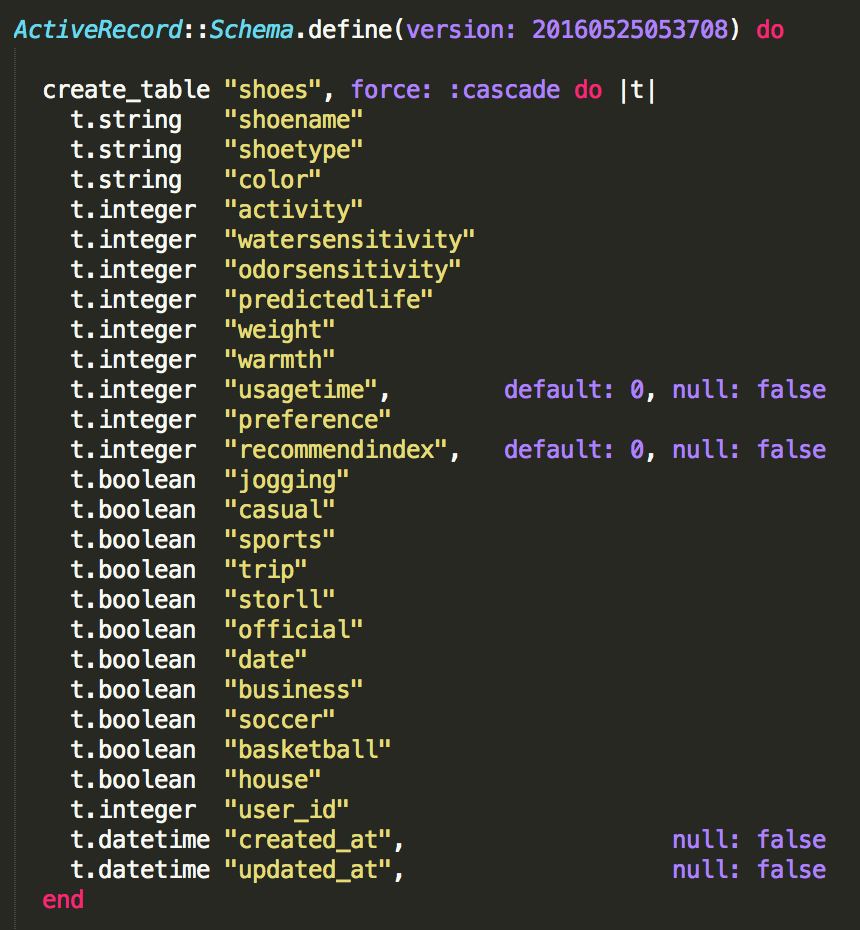
\includegraphics[scale=0.52]{schemashoes}
  \caption{Modeling Shoes in database}\label{fig:label}
\end{center}
\end{figure}
\begin{figure}[H]
\begin{center}
    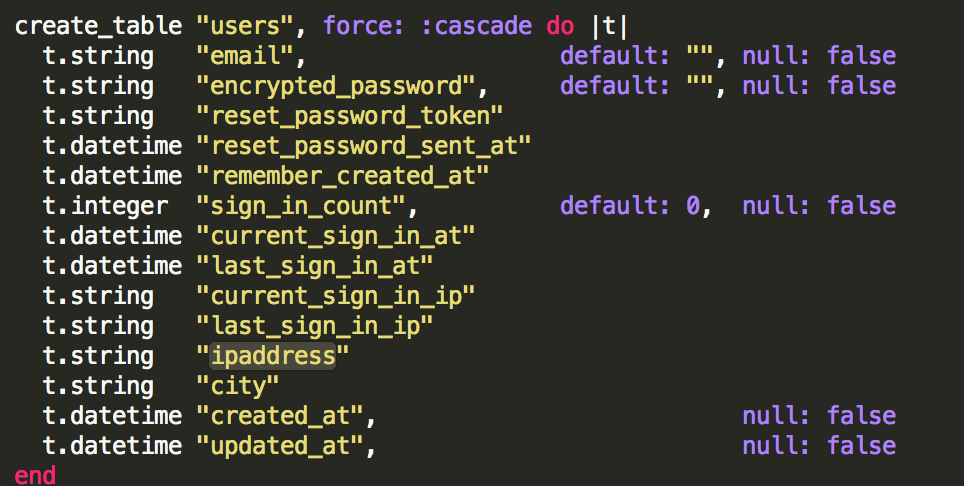
\includegraphics[scale=0.48]{schemausers}
  \caption{Modeling Users in database}\label{fig:label}
\end{center}
\end{figure}
\subsubsection{Purpose} The purpose of using the Ruby on Rails is to provide a easily accessed user interaction environment through web service. IoT will be realized through the web service, since it will let the user to take care of their shoes anytime, anywhere. So we have decided to use the Ruby on Rails application framework.
\subsubsection{Functionality} There are several functionalities for the Ruby on Rails module. First user is able to check the status of the Smart Shoebox. The status contains the meaning of temperature and humidity. Second, the users are able to check the weather outside so that he or she could choose the proper shoes. Third with the weather information and the shoes information saved in the database recommendation function will be realized. Fourth, using the wifi, it will control the Smart Shoebox remotely. Last but not least, with Ruby on rails, the user information will be saved and managed in the database.
\subsubsection{Location of Source Code}/project/shoebox/website
\subsubsection{Class component} Ruby on Rails use the so called MVC model to specify the events and actions of the web service. M satnds for model, where we save and use the data of the user and shoes. (You can easily think of a database table when we develop web service.)V stands for view, which takes care of the visualization of the html. It is the factors forming the front end of the web service. (HTML, CSS, JAVASCRIPT) C stands for controller and it takes care of the actions, receiving requests from the users and look up for the data from the model and visualizae through the view.

The user accesses the Smart Shoebox's URL and send request. Then the 'Controller' receives the request and look up the 'Model' and bring the data from the database. At last with the data brought from the model, 'View' visualizes so that the user can see.

\subsubsection{Where it is taken from}It is taken from the rails installer site. RailsInstaller is the quickest way to go from zero to developing Ruby on Rails applications. 
 
(http://railsinstaller.org/en)
\subsubsection{How and Why we use it} Based on the Ruby programming language and MVC model we make a web service for the users of the Smart Shoebox. It is possible to developing a web service from scratch, but it is not a good idea to do so, when it is so important and emphasized to use an open sources. Application framework for the Ruby language is already provided and we have decided to build on top of it.
\begin{figure}[H]
\begin{center}
    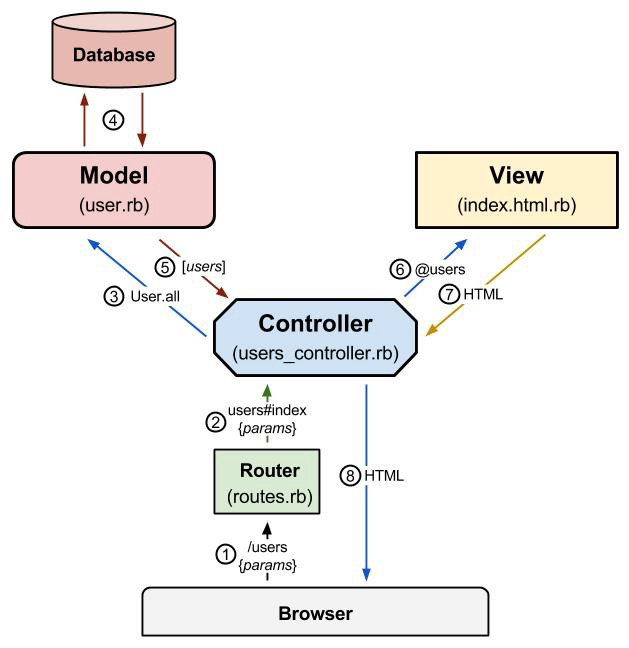
\includegraphics[scale=0.42]{mvc}
    \caption{MVC} \label{fig:label}
\end{center}
\end{figure}
% 6. use cases
\section{Use Cases}
\subsection{Use case 1 : Setup} This case is for the users using the Smart Shoebox for the first time.  If it is the first time for the user to use Smart Shoebox, you have to sign up for the website. If you are already registered, you can login with your id and password.
%image15
\begin{figure}[H]
\begin{center}
    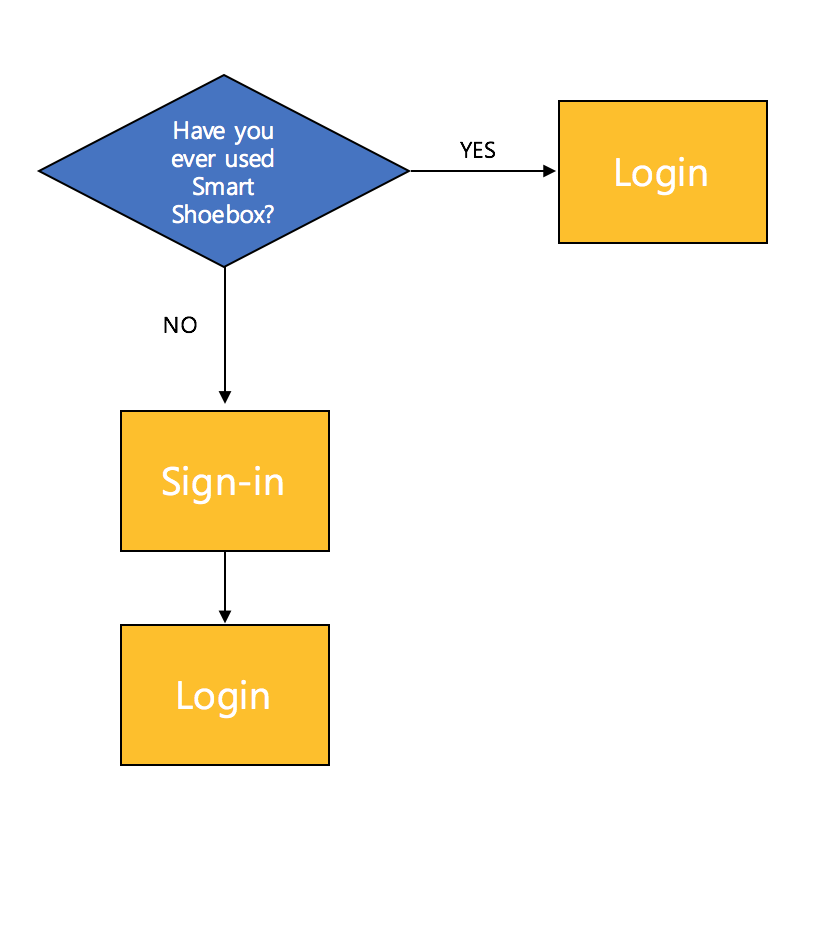
\includegraphics[scale=0.7]{usecase1}
    \caption{Use case 1 : Setup} \label{fig:label}
\end{center}
\end{figure}
%image
\begin{figure}[H]
\begin{center}
    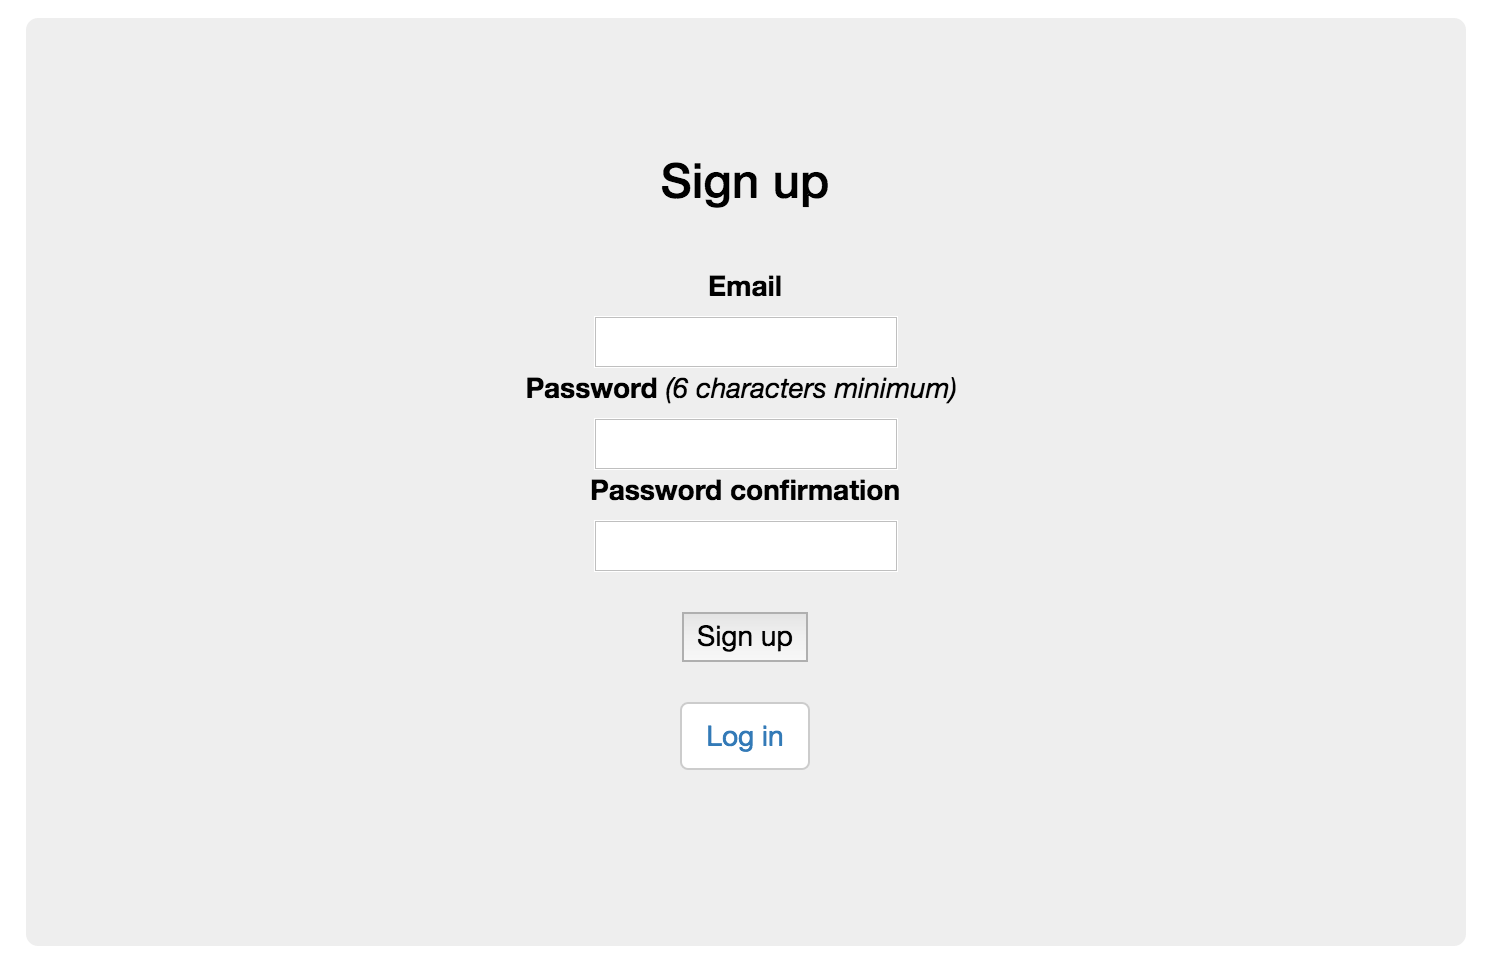
\includegraphics[scale=0.3]{capture1}
     \caption{Sign up page}\label{fig:label}
\end{center}
\end{figure}
%image
\begin{figure}[H]
\begin{center}
    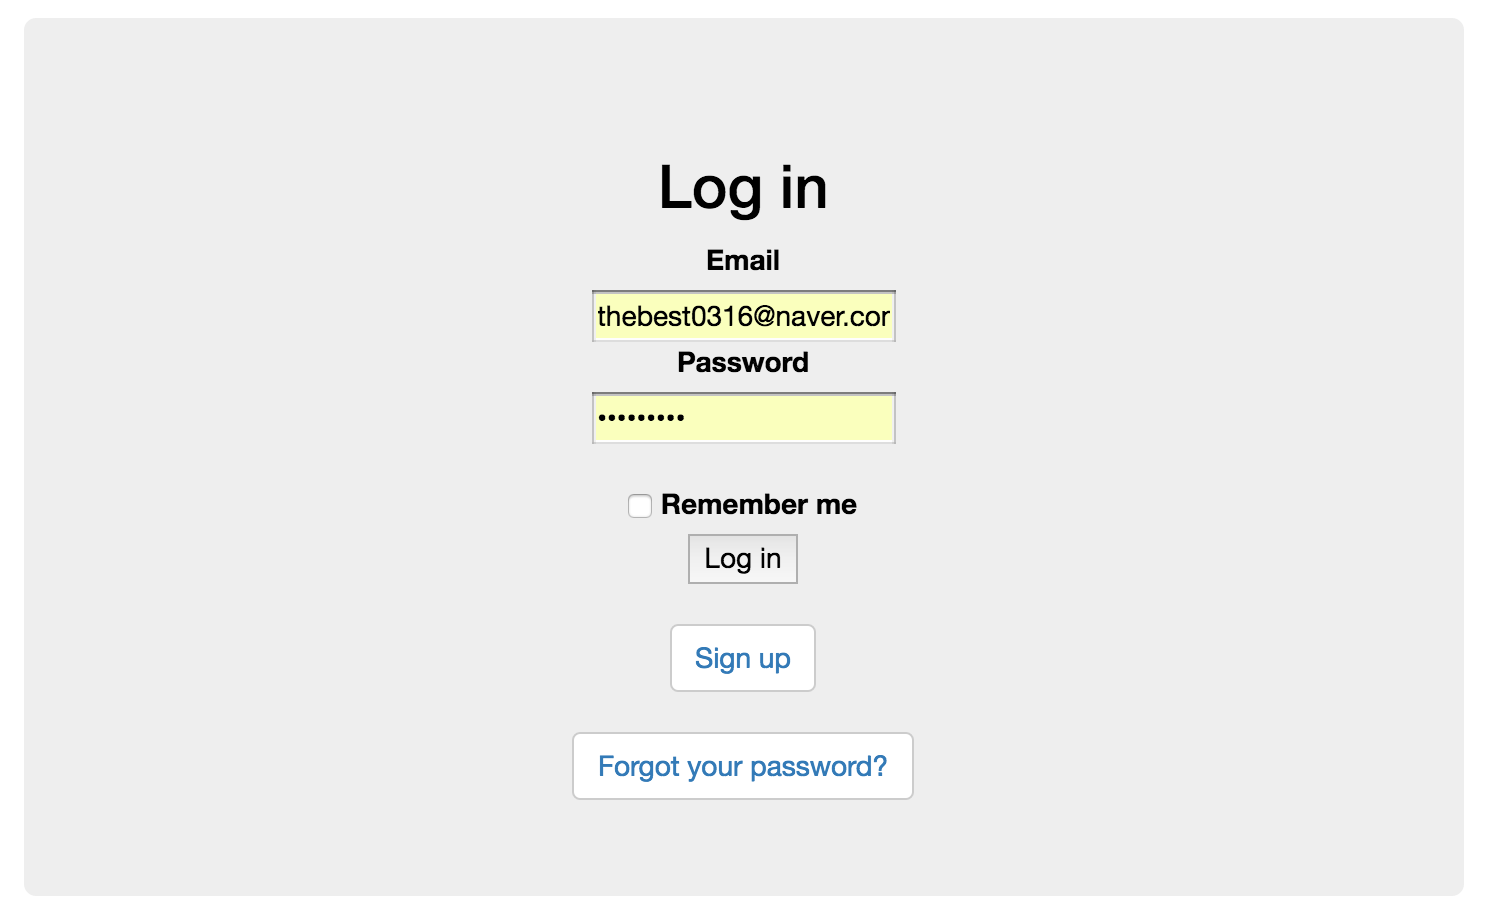
\includegraphics[scale=0.3]{capture2}
     \caption{Log in page}\label{fig:label}
\end{center}
\end{figure}
%image
\begin{figure}[H]
\begin{center}
    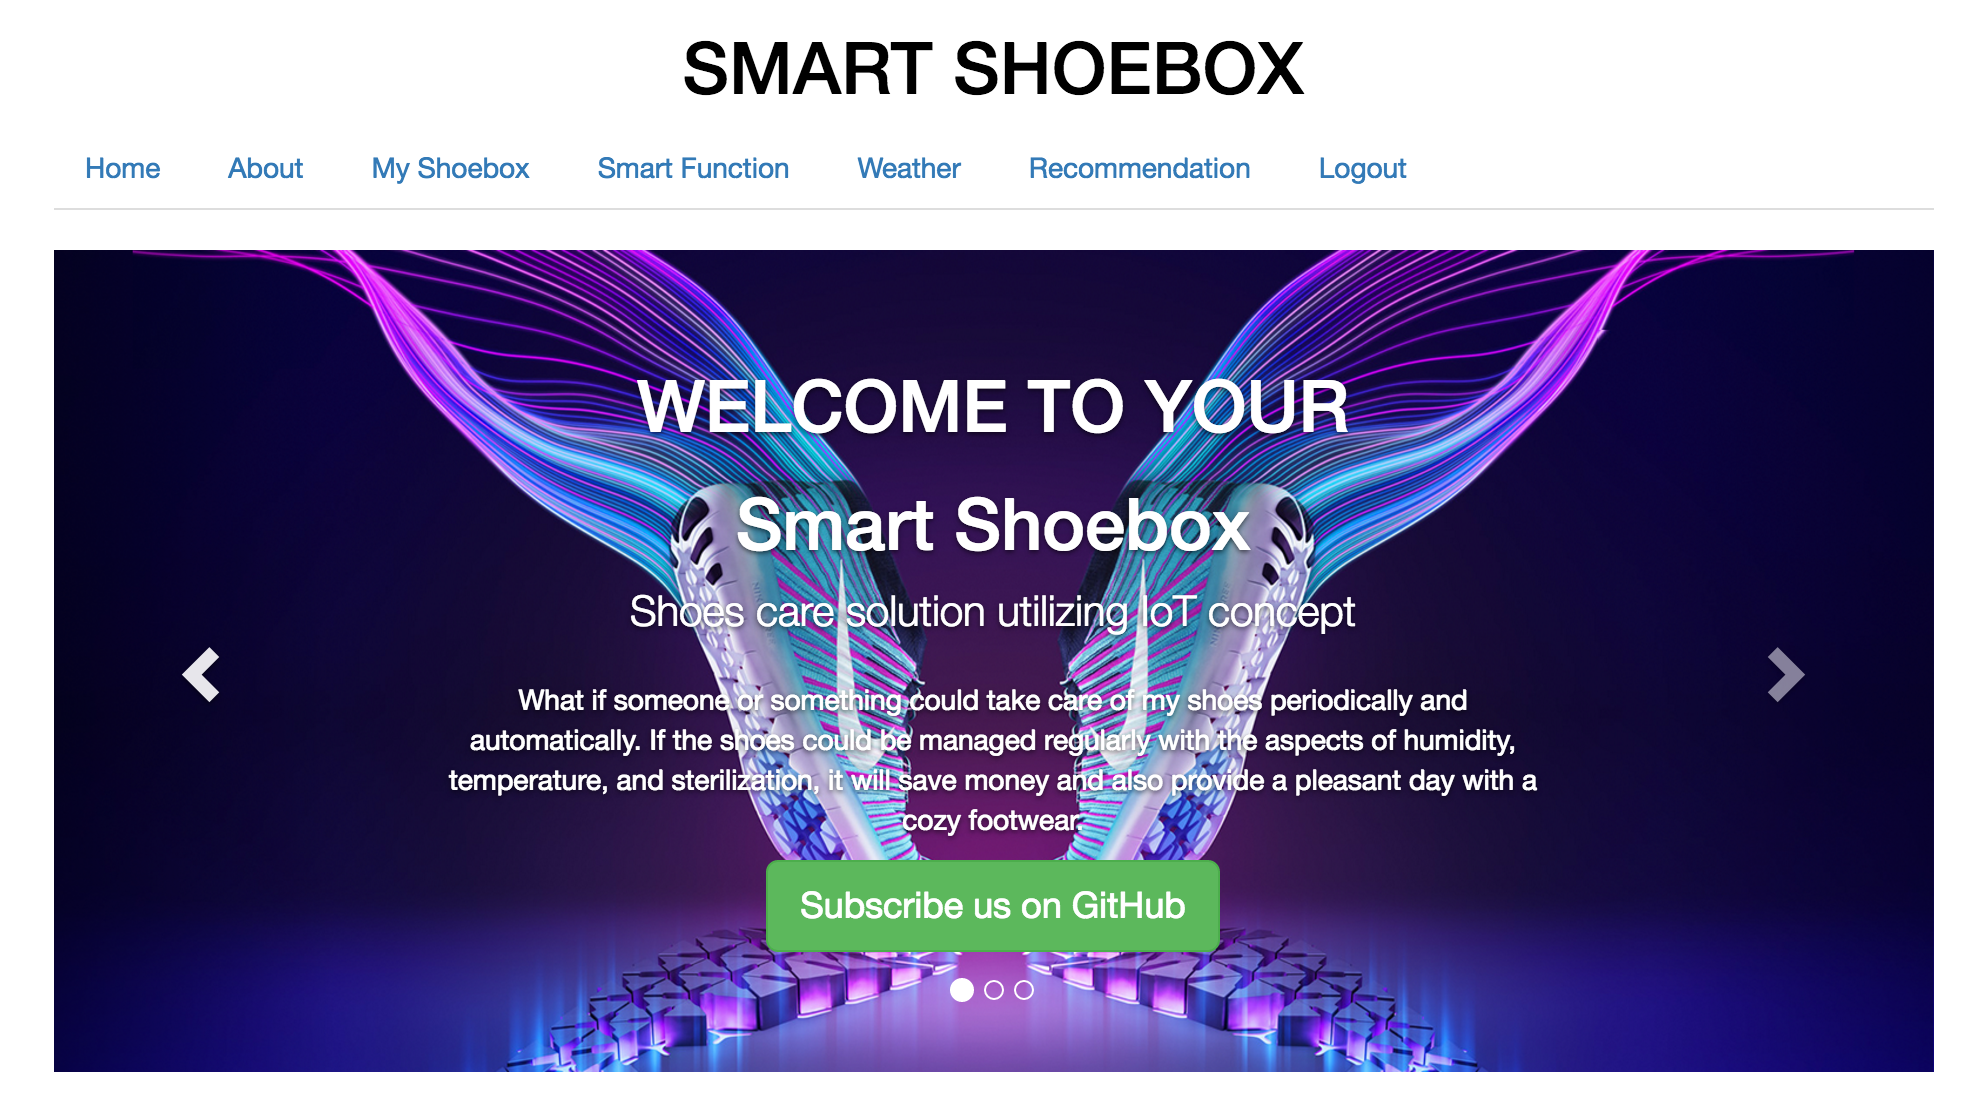
\includegraphics[scale=0.25]{capture3}
     \caption{After logging in}\label{fig:label}
\end{center}
\end{figure}

\subsection{Use case 2 : Users request for a Smart function} This case is taking care of the needs of the user to use the smart function of the Smart Shoebox. (Optimization, Drying, Sterilization, Deodorization) After the use case one, the user is in the website. You can click on the Smart function tab on the top. In the page of Smart function, you have to type in the IP address of the Smart Shoebox. After typing in the IP addresses, all the user has to do is click the function which the user needs. You can use the functions as long as you want and click the button again to turn it off.
%image16
\begin{figure}[H]
\begin{center}
    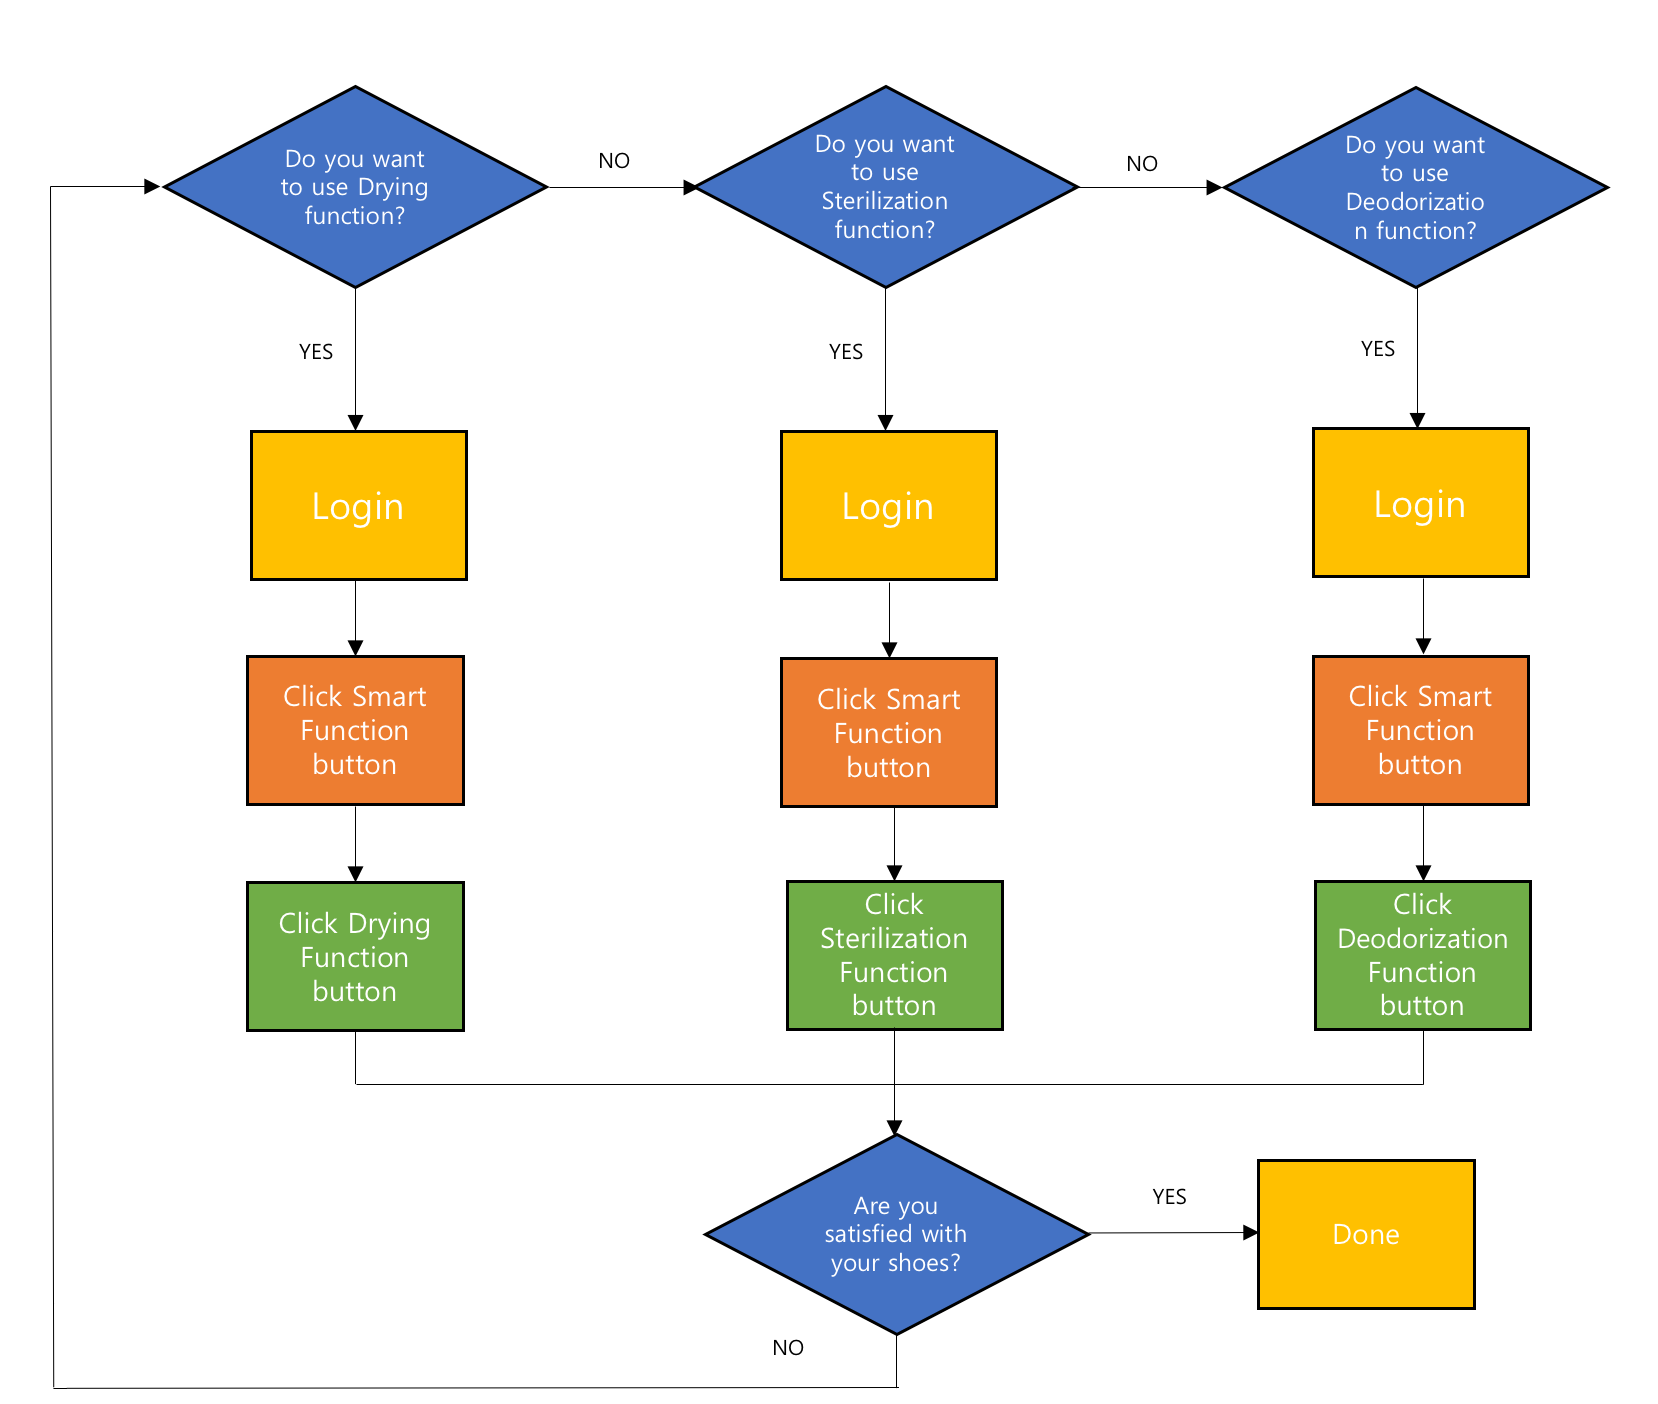
\includegraphics[scale=0.3]{usecase2}
    \caption{Use case 2 : Users request for a Smart function} \label{fig:label}
\end{center}
\end{figure}
%image
\begin{figure}[H]
\begin{center}
    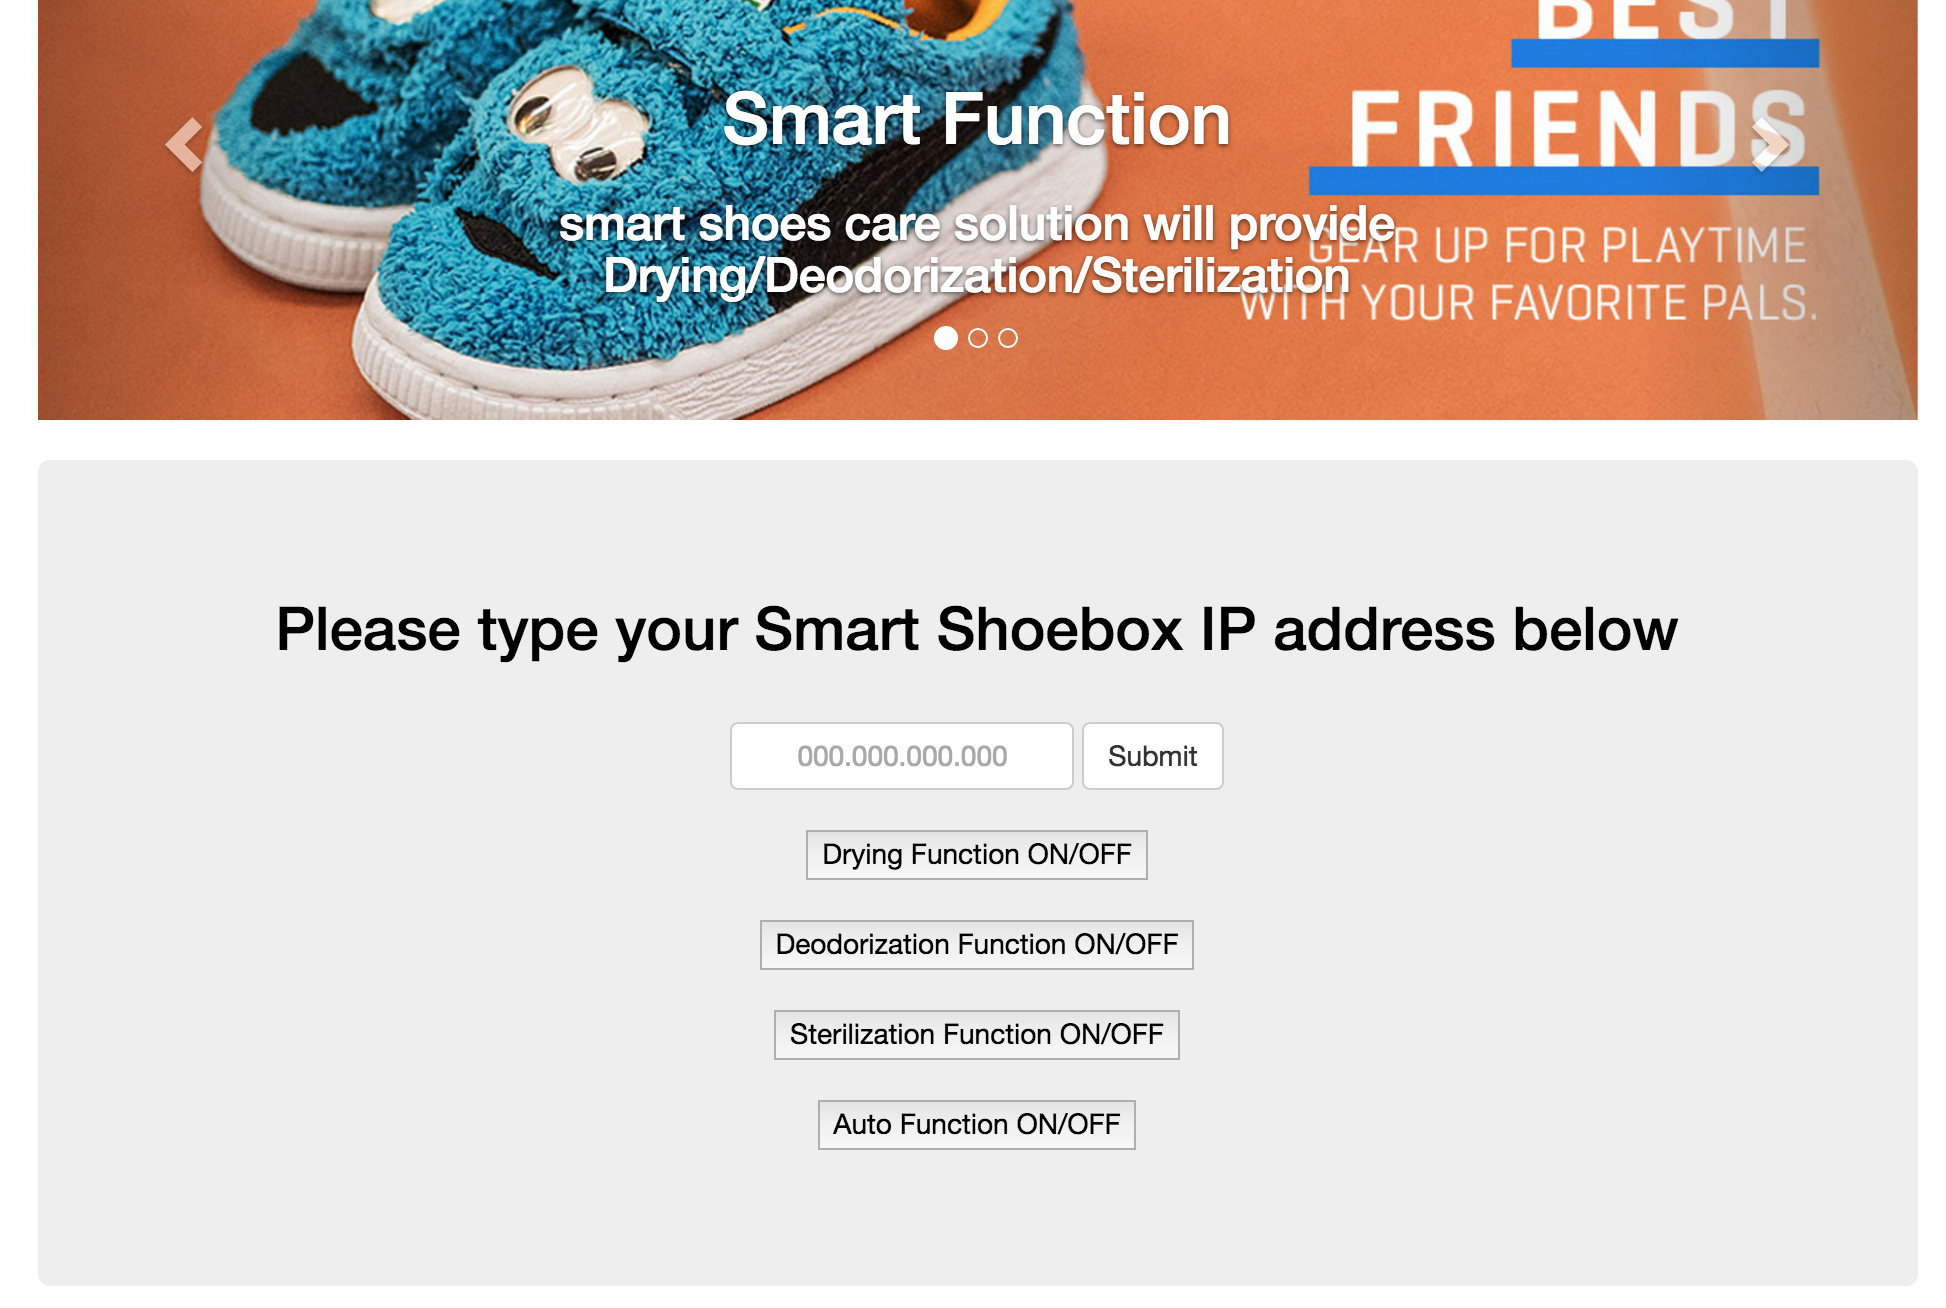
\includegraphics[scale=0.25]{capture4}
    \caption{Smart function page} \label{fig:label}
\end{center}
\end{figure}
\subsection{Use case 3 : Users request for the weather forecast} This case is taking care of the needs of the user to see the weather. After the use case one, the user is in the website. You can click on the Weather tab on the top. In the page of Weather, the user can choose the city, which he or she is interested in. There are few cities of South Korea provided.
%image17
\begin{figure}[H]
\begin{center}
    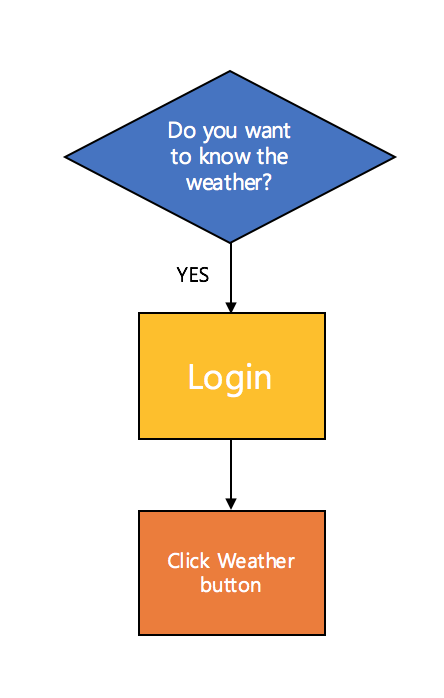
\includegraphics[scale=0.8]{usecase3}
    \caption{Use case 3 : Users request for the weather forecast} \label{fig:label}
\end{center}
\end{figure}
%image
\begin{figure}[H]
\begin{center}
    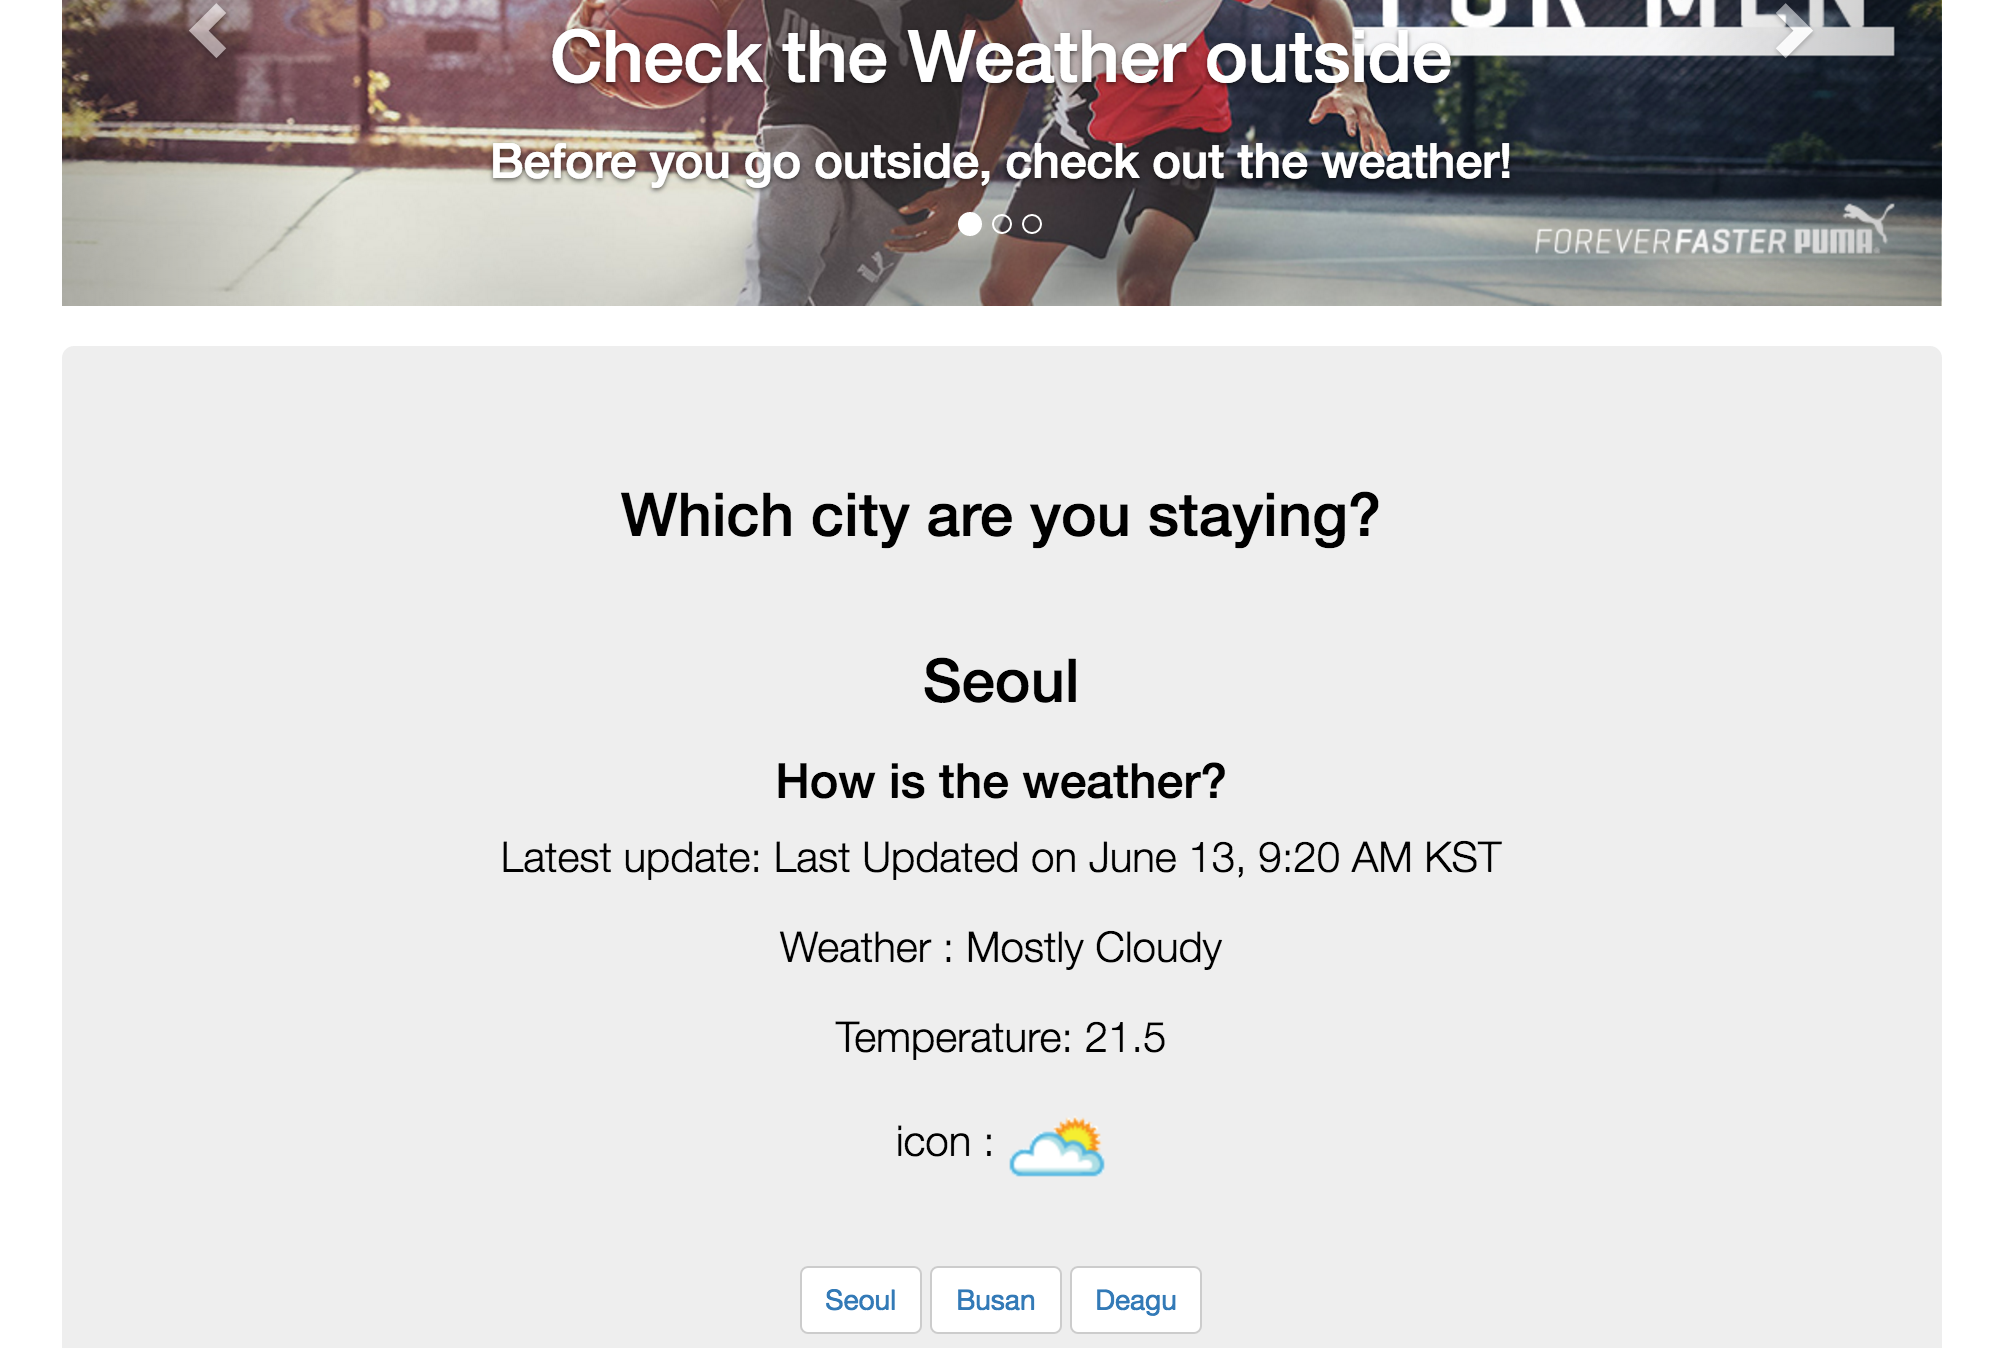
\includegraphics[scale=0.25]{capture5}
    \caption{Weather page} \label{fig:label}
\end{center}
\end{figure}

\subsection{Use case 4 : Users request for Recommendation} This case covers the needs of the user to receive a recommendation of the shoes. After the use case one, the user is in the website. You can click on the Recommendation tab on the top. In the page of Recommendation, the user can choose the main activity and the city, which he or she is staying or panning to go. After selecting these two, the user submits. Based on the two information, the website provides recommendation points for each shoes.
%image18
\begin{figure}[H]
\begin{center}
    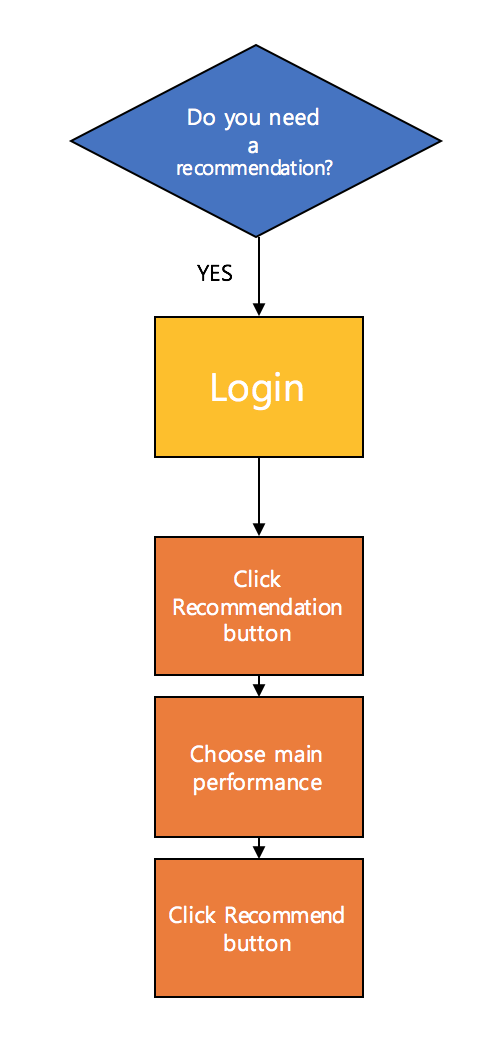
\includegraphics[scale=0.8]{usecase4}
    \caption{Use case 4 : Users request for Recommendation} \label{fig:label}
\end{center}
\end{figure}
%image
\begin{figure}[H]
\begin{center}
    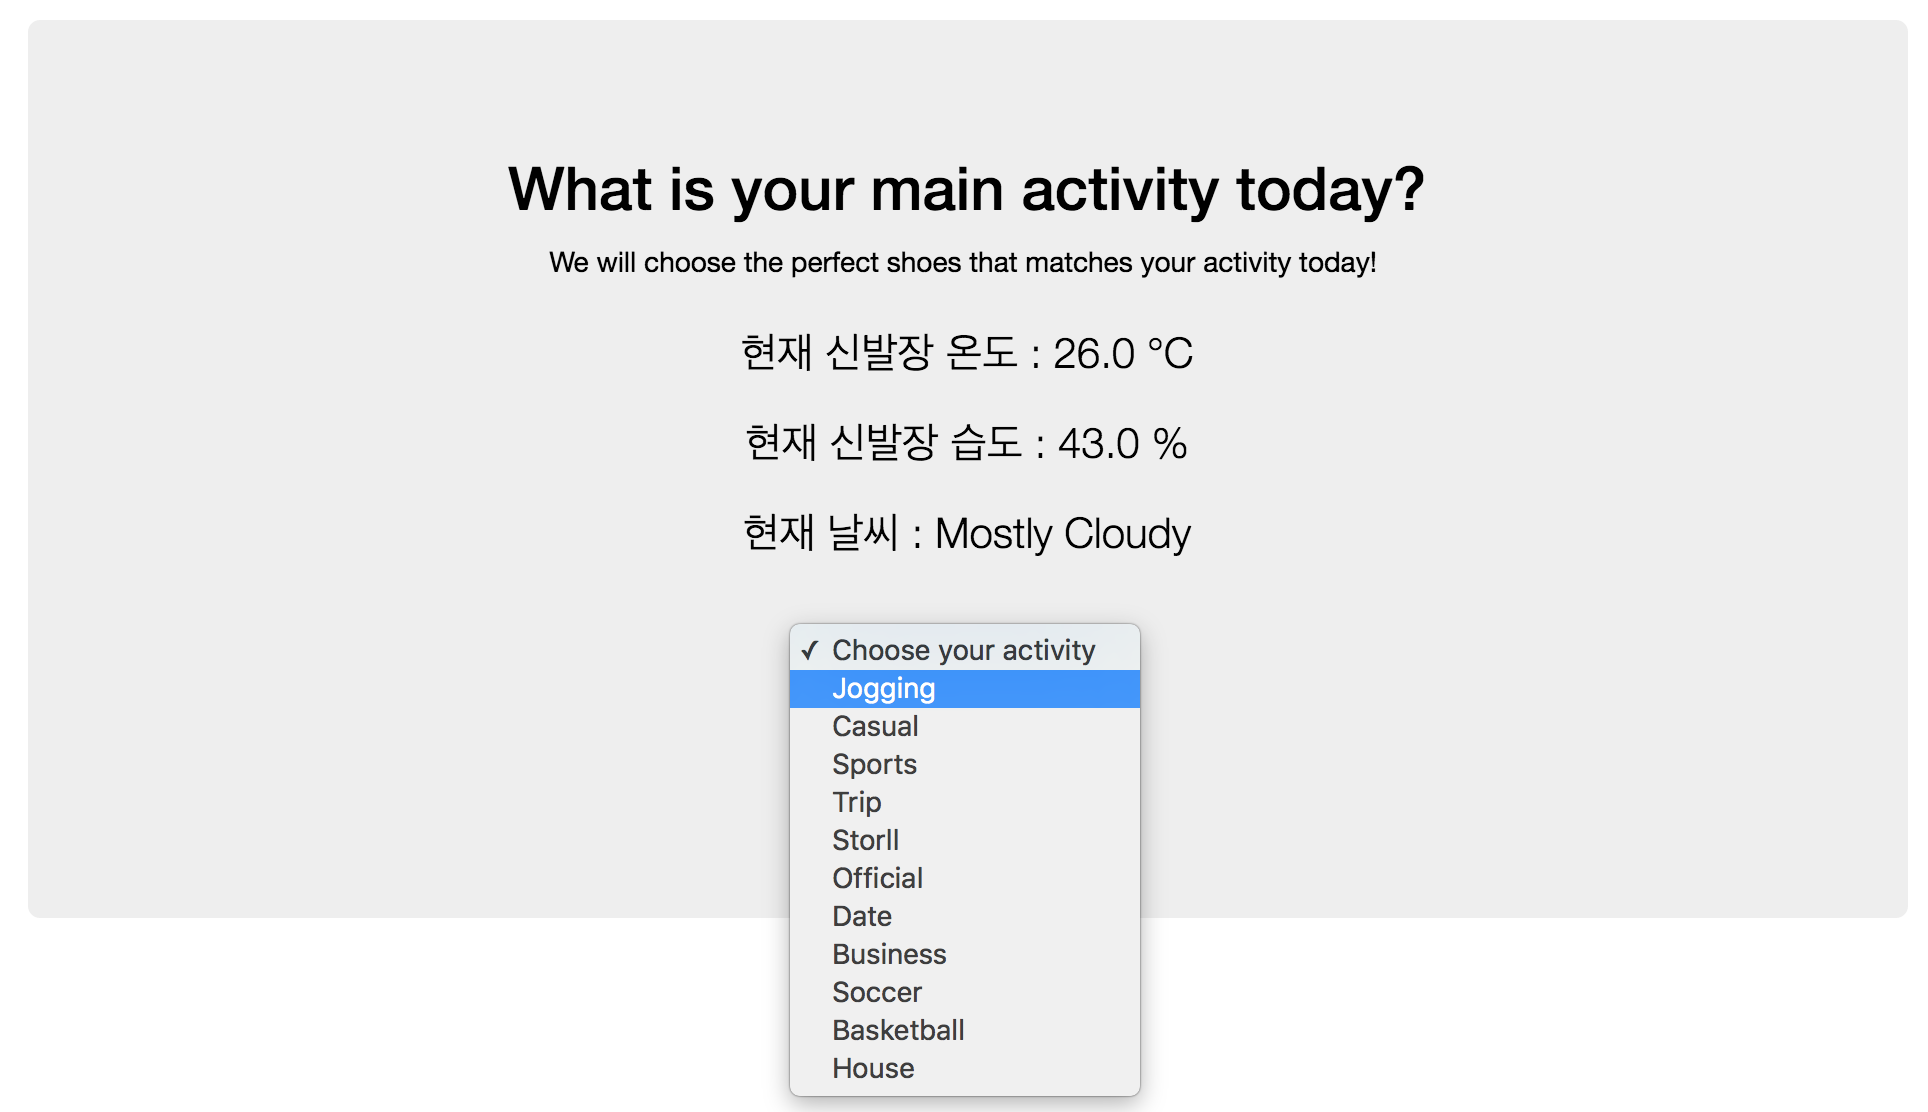
\includegraphics[scale=0.25]{capture6}
    \caption{Recommendation page} \label{fig:label}
\end{center}
\end{figure}
\subsection{Use case 5 : Adding the shoes to the Smart Shoebox} This case is to explain the process for the user adding the shoes to the Smart Shoebox. After the use case one, the user is in the website. You can click on the My shoebox tab on the top. In the page of My shoebox, the user can add the items the user possess. 
%image
\begin{figure}[H]
\begin{center}
    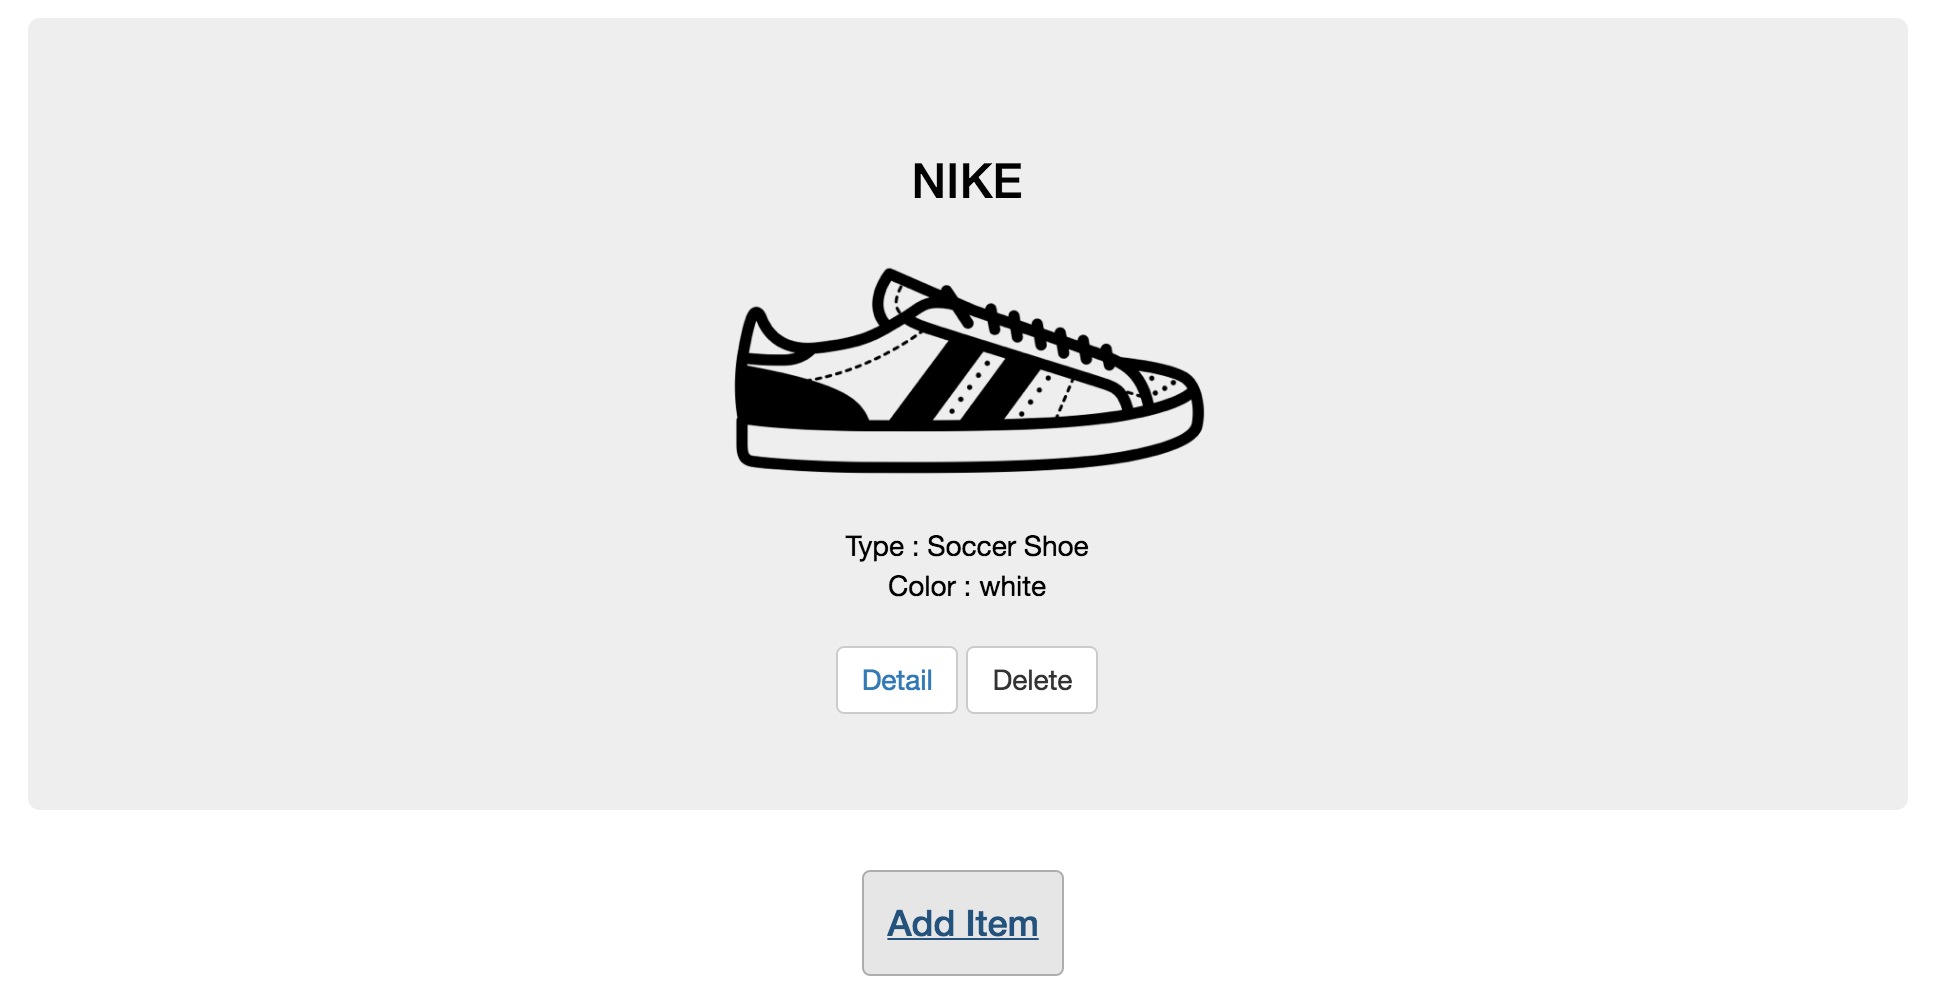
\includegraphics[scale=0.26]{capture7}
    \caption{My Shoebox page} \label{fig:label}
\end{center}
\end{figure}
%image
\begin{figure}[H]
\begin{center}
    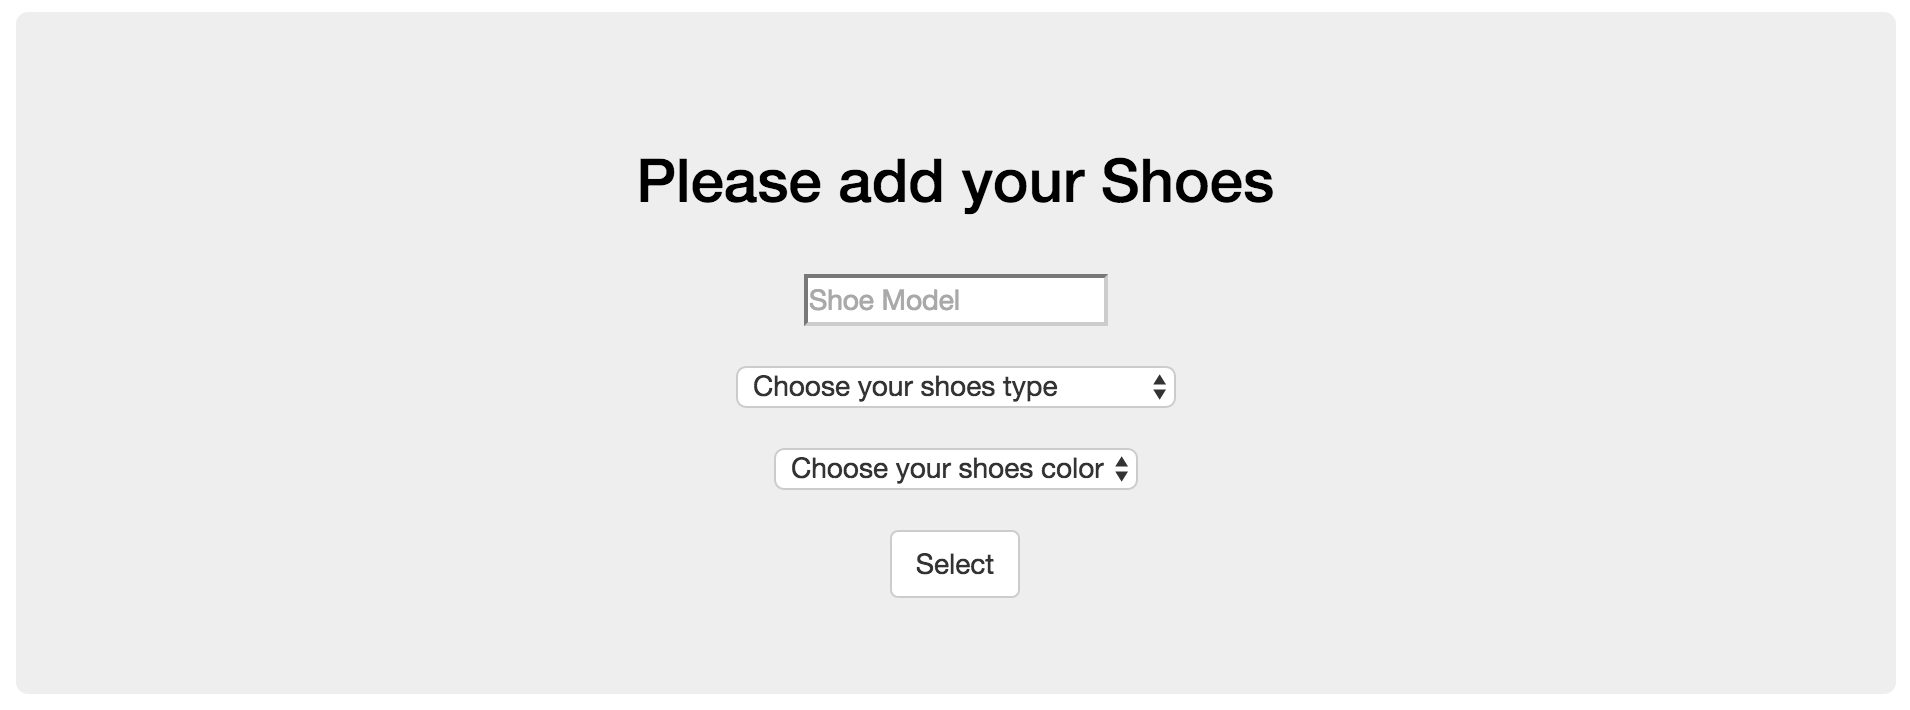
\includegraphics[scale=0.26]{capture8}
    \caption{Adding a new item to Smart Shoebox} \label{fig:label}
\end{center}
\end{figure}
\subsection{Use case 6 : Users request for detail information about the shoes} This case covers the needs of the user to see the detail information of the shoes contained in the Smart Shoebox. After the use case one, the user is in the website.  After the use case one, the user is in the website. You can click on the My shoebox tab on the top. In the page of My shoebox, the user can choose the shoes he or she is interested in. If the user click the detail button each attached to the added item, the user can see all the detailed additional information.
%image19
\begin{figure}[H]
\begin{center}
    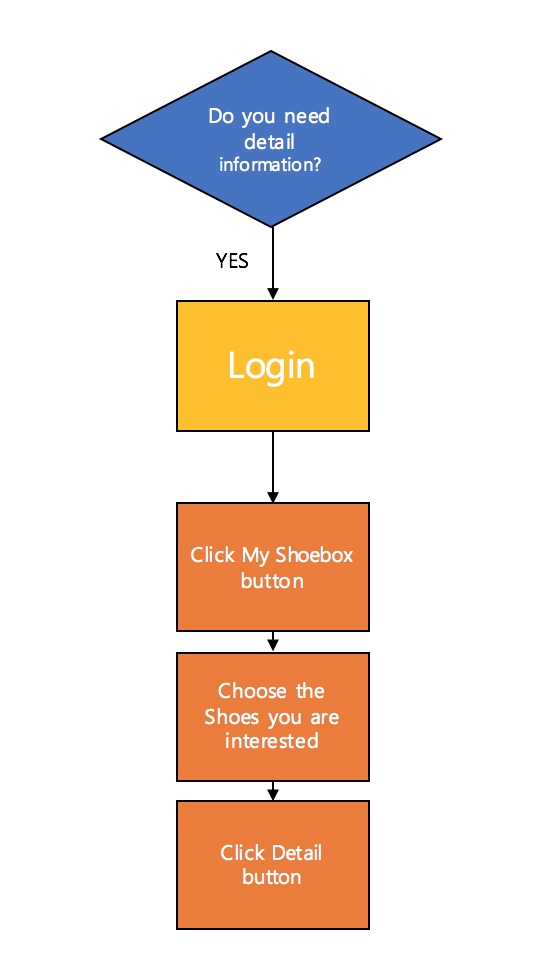
\includegraphics[scale=0.8]{usecase5}
    \caption{Use case 6 : Users request for detail information about the shoes} \label{fig:label}
\end{center}
\end{figure}
% 7. installation guide
\section{Installation guide}
\subsection{Introduction}
This is the Step-by-Step Guide to software installation and maintenance. Actually, Smart Shoebox is activated through the website. Because of this feature of IoT, it seems to be simple and easy for the installation. But still there are several steps to follow to install the Smart Shoebox software.
\subsection{Installation procedure}
\subsubsection{Step1: Arduino Setting and Smart Shoebox Setting}
First we have to set the data for the used wifi and password inside the Arduino code. As you can See in Fig. 28.  (AndroidHotspot5051 and rbgur123) this part is setting the environment for the Smart Shoeboxes wifi.
\begin{figure}[H]
\begin{center}
    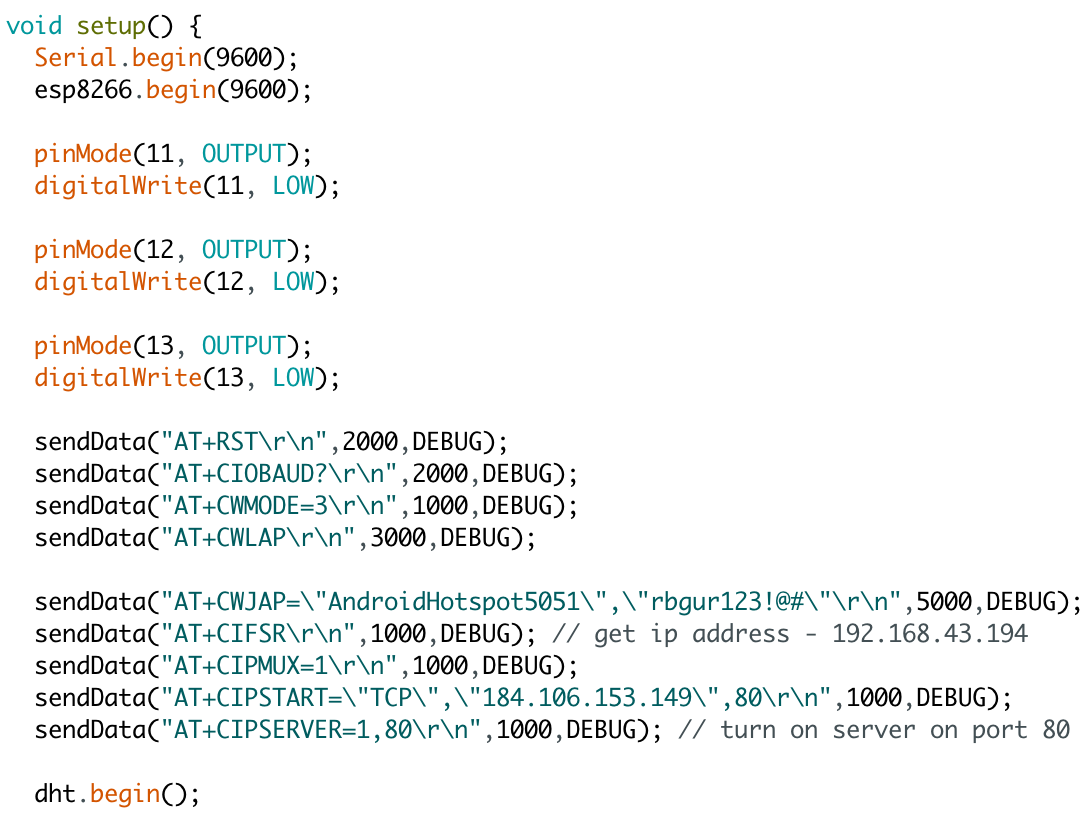
\includegraphics[scale=0.47]{step1}
    \caption{Step1:Arduino Setting and Smart Shoebox Setting} \label{fig:label}
\end{center}
\end{figure}
\subsubsection{Step2: Website Sign-up}
After the Arduino part is handled we have the Smart Shoebox in hand. Now we can communicate through website. We have to go into the website and sign up. As you can see in Fig. 29. you can easily sign up by typing email address and password.
\begin{figure}[H]
\begin{center}
    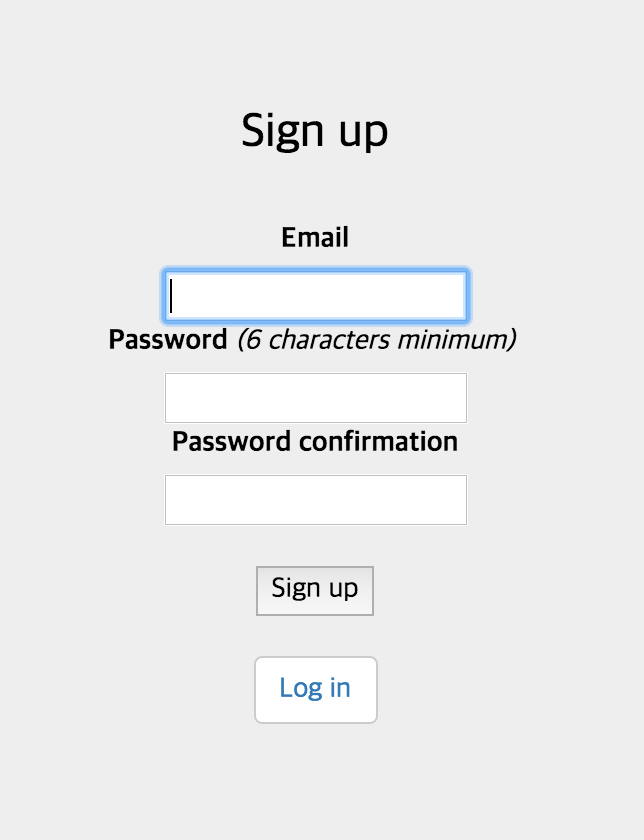
\includegraphics[scale=0.65]{step2}
    \caption{Step2: Website Sign-up} \label{fig:label}
\end{center}
\end{figure}
\subsubsection{Step3: Login}
After we sign up for the Smart Shoebox website, we have to login to the website. Type in the email address and password. We will be in the main page of the website.
\begin{figure}[H]
\begin{center}
    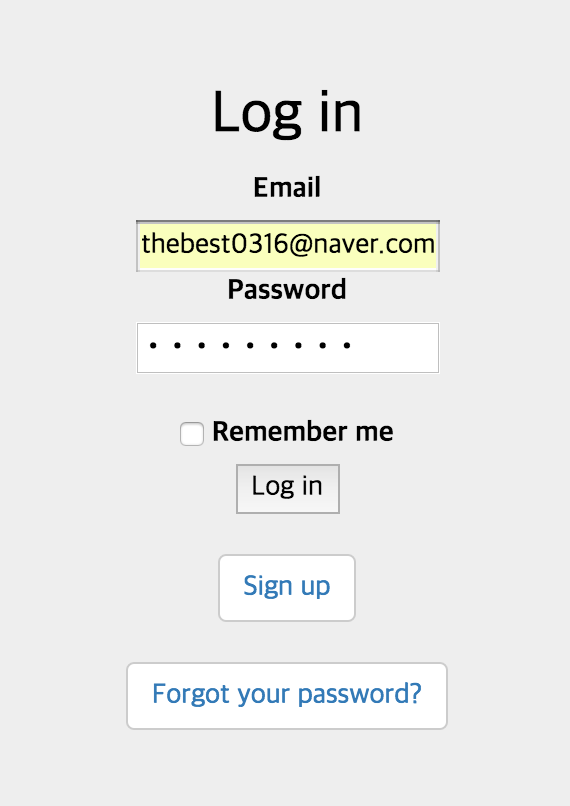
\includegraphics[scale=0.7]{step3}
    \caption{Step3: Login} \label{fig:label}
\end{center}
\end{figure}
\subsubsection{Step4: Setting the IP address in website}
After we login for the Smart Shoebox website, we have to set the IP address in the website. Click the Smart function tab and there is a blank where we can type in the IP address of the Smart Shoebox.
\begin{figure}[H]
\begin{center}
    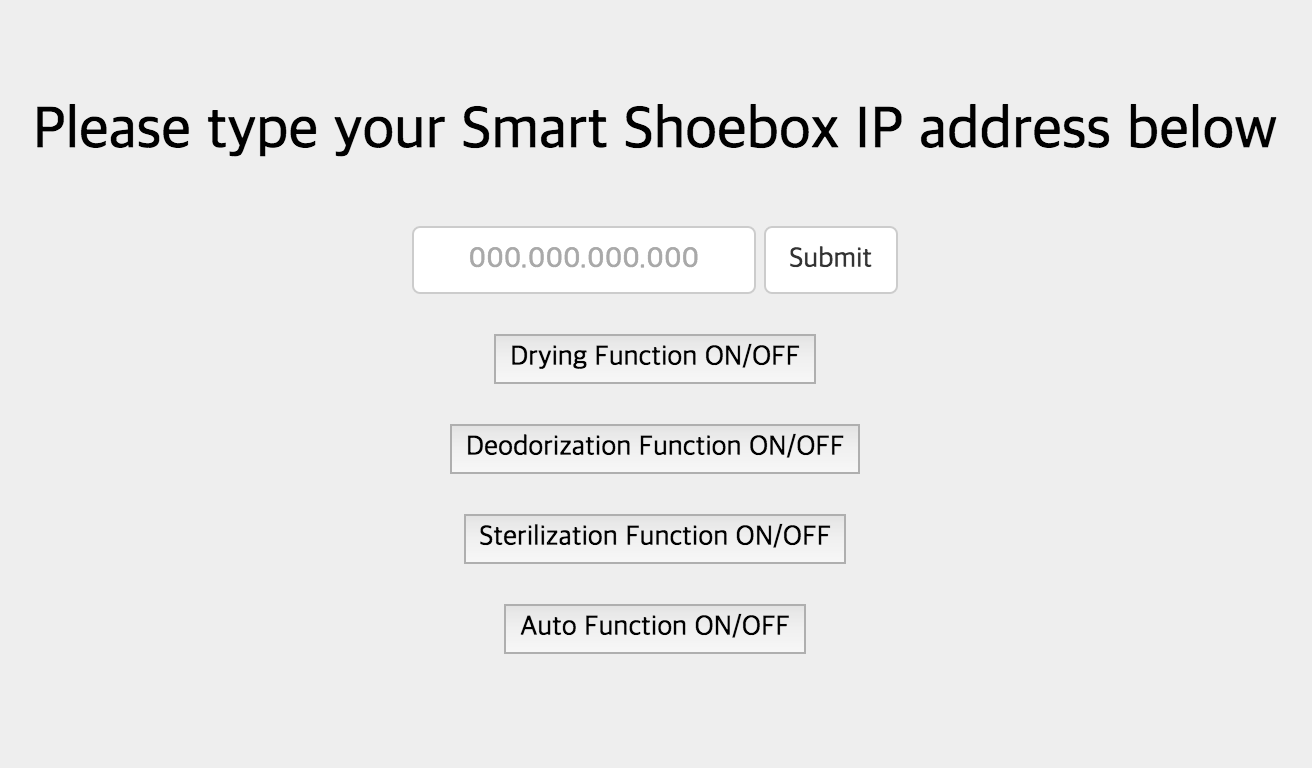
\includegraphics[scale=0.35]{step4}
    \caption{Step4: Setting the IP address in website} \label{fig:label}
\end{center}
\end{figure}
\subsubsection{Step5: Thing Speak sign up}
Thing Speak is the website, help us receive the temperature and humidity of the Smart Shoebox in realtime. We need to sign up for this website also.
\begin{figure}[H]
\begin{center}
    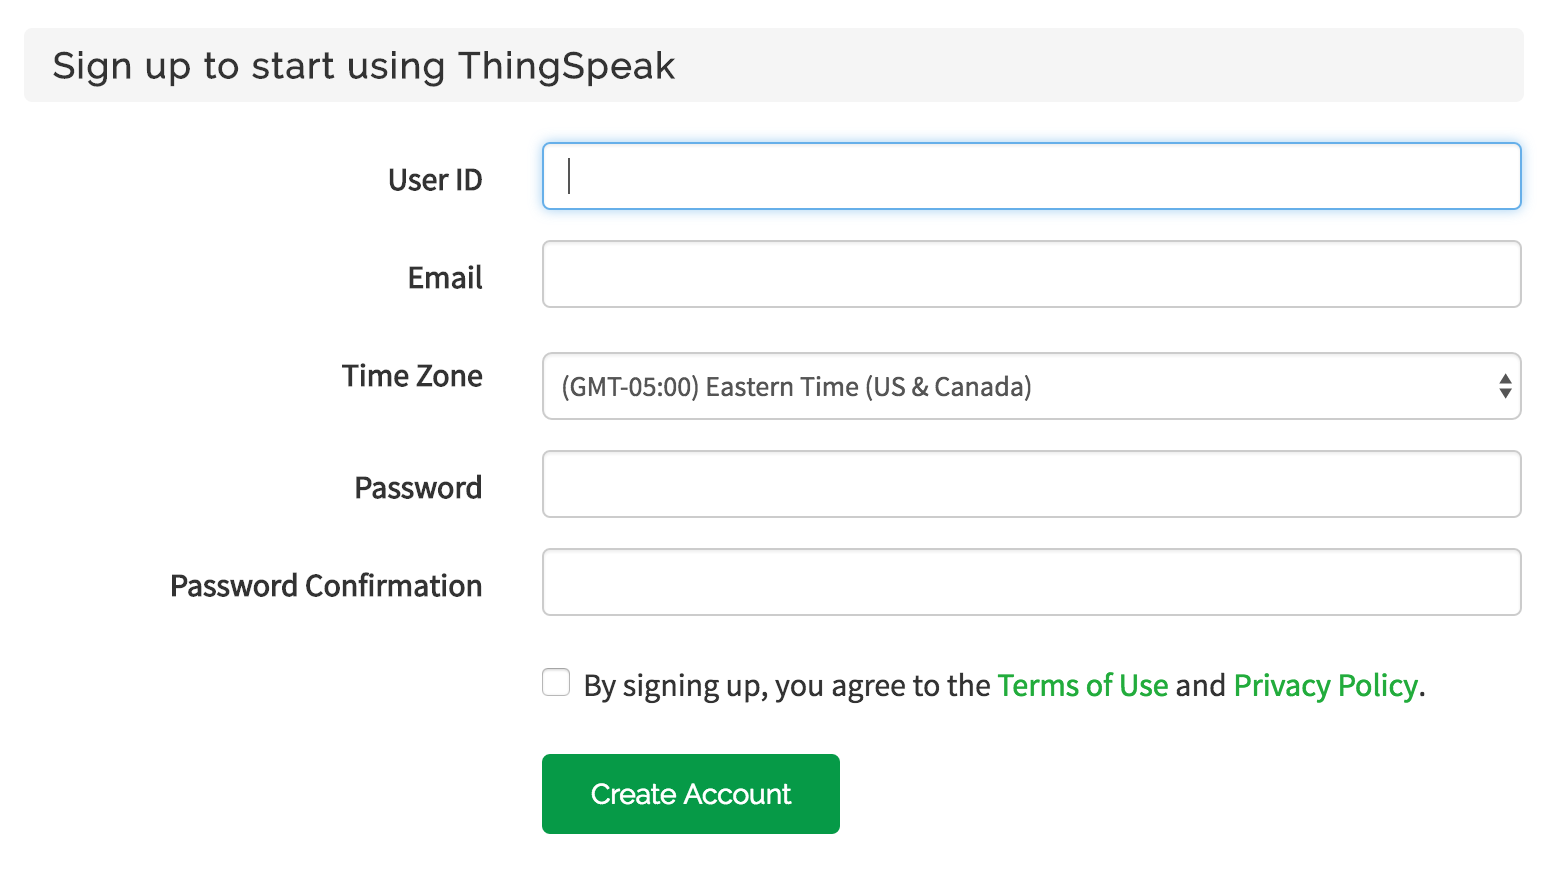
\includegraphics[scale=0.35]{step5}
    \caption{Step5: Thing Speak sign up} \label{fig:label}
\end{center}
\end{figure}
\subsubsection{Step6: Extracting the API key}
After signing up for the Thing Speak, we have to extract the API key to let the website and Smart Shoebox to communicate. This step will allow the Arduino sensor information to reach Thing Speak, and Thing Speak will send the information to the Smart Shoebox website.
\begin{figure}[H]
\begin{center}
    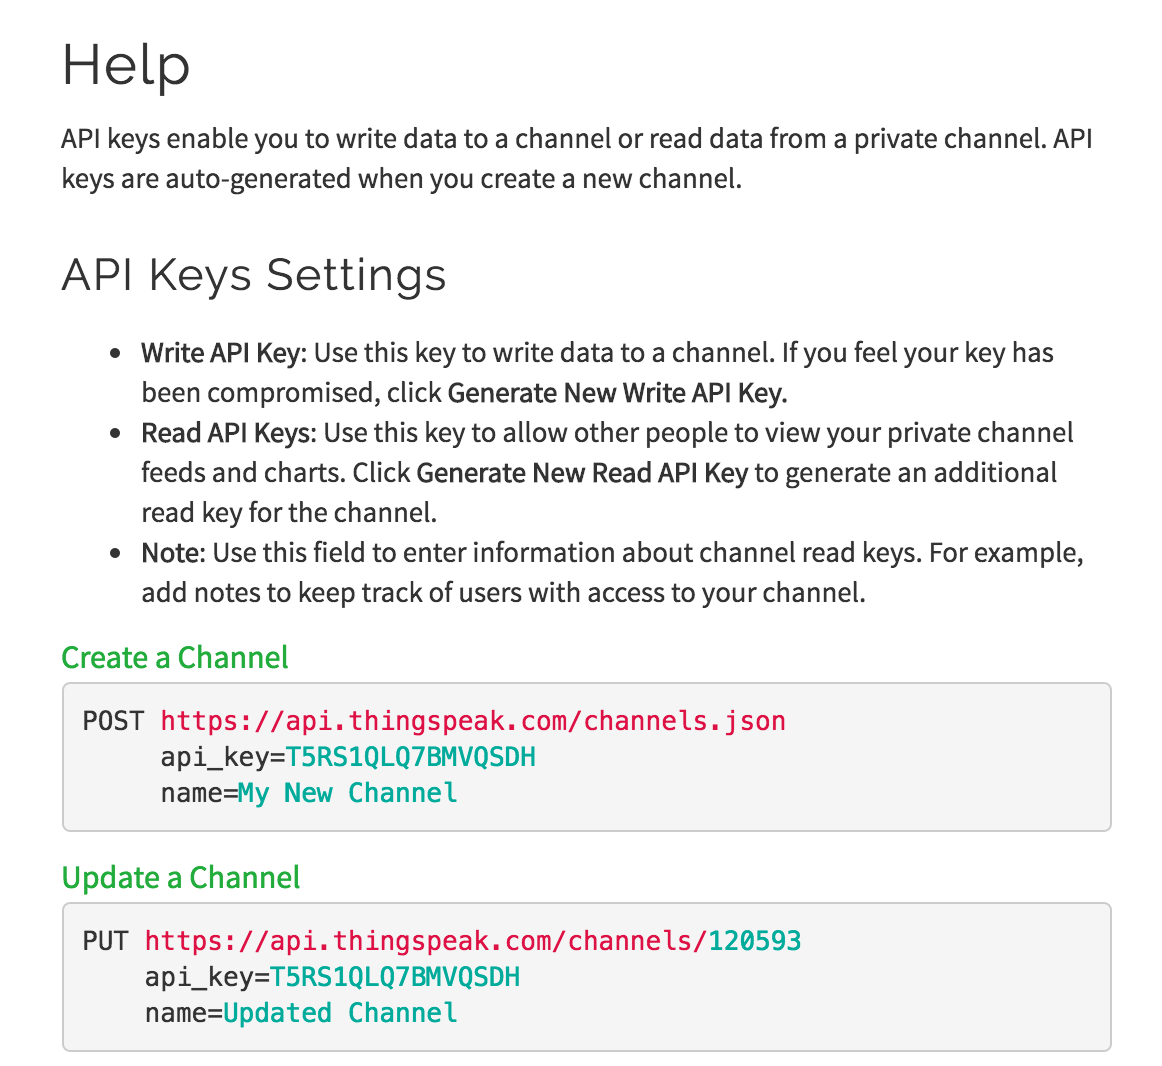
\includegraphics[scale=0.4]{step6}
    \caption{Step6: Extracting the API key} \label{fig:label}
\end{center}
\end{figure}
\begin{figure}[H]
\begin{center}
    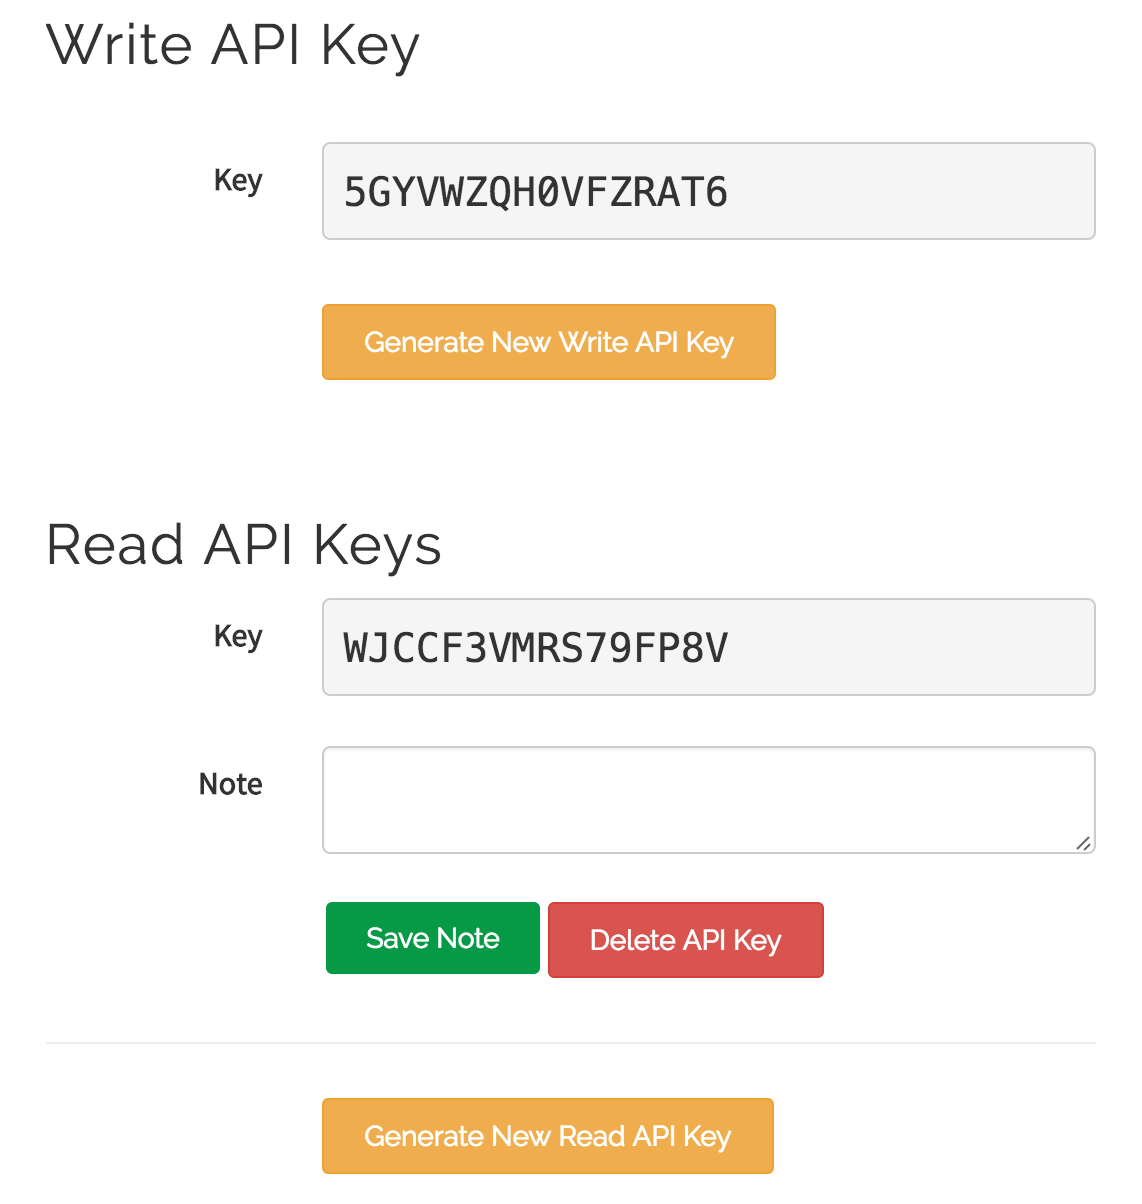
\includegraphics[scale=0.4]{step61}
    \caption{Step6: Extracting the API key} \label{fig:label}
\end{center}
\end{figure}
\subsubsection{Step7: Inserting the API key into the Website}
After letting the communication between Smart Shoebox and Thing Speak and website all in one, we have use the API and channel to show the real time information of the Smart Shoebox. The user can easily see the temperature and humidity changing in the Smart function page.
\begin{figure}[H]
\begin{center}
    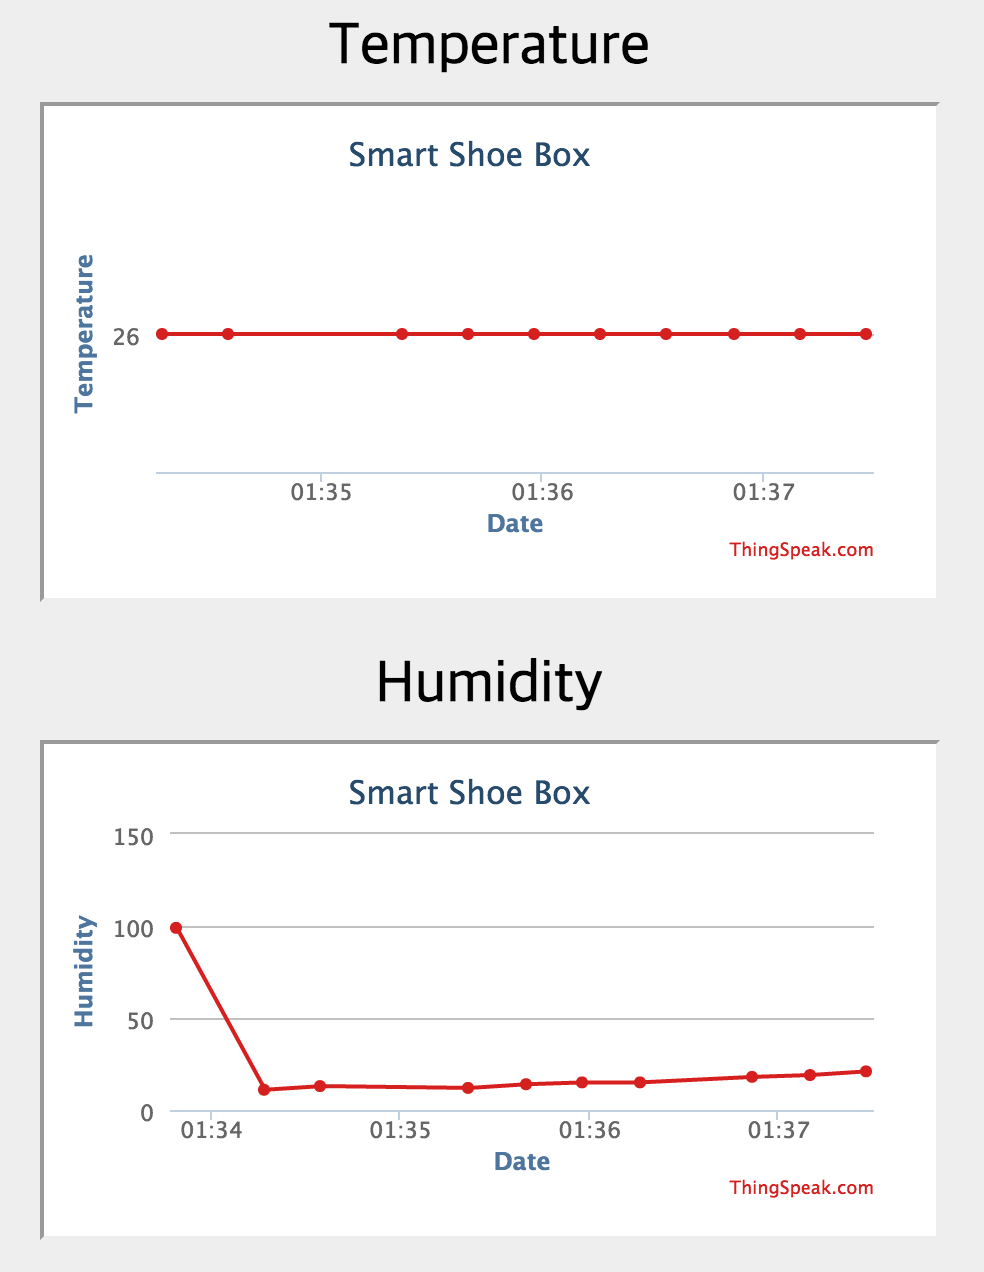
\includegraphics[scale=0.45]{step7}
    \caption{Step7: Extracting the API key and showing the realtime graph} \label{fig:label}
\end{center}
\end{figure}
\begin{figure}[H]
\begin{center}
    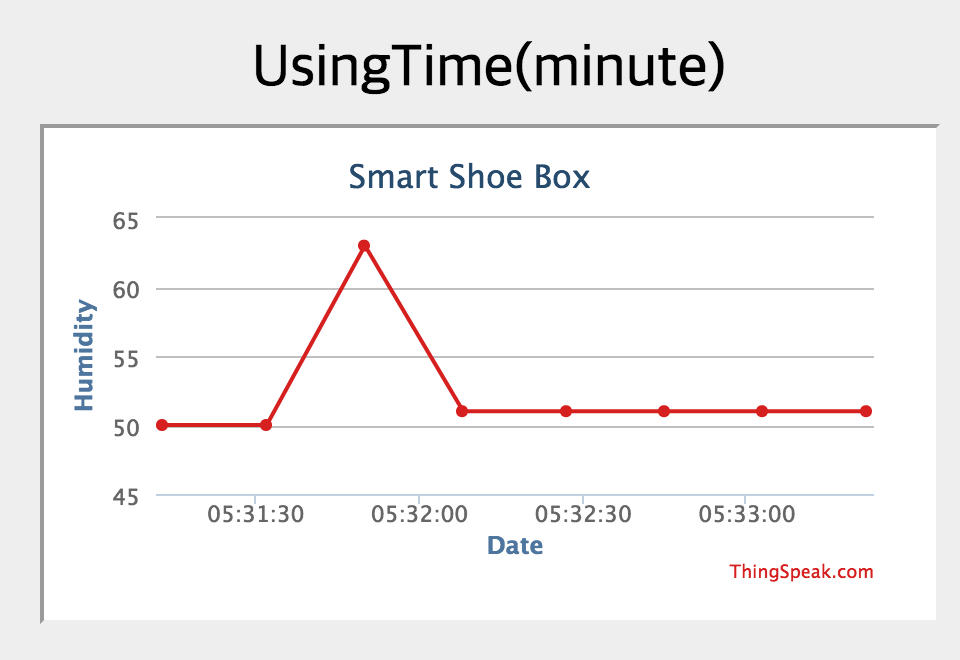
\includegraphics[scale=0.45]{usingtime}
    \caption{Step7: Extracting the API key and showing the realtime graph} \label{fig:label}
\end{center}
\end{figure}
% 8. Discussion
\section{Discussion}
%Write one or more paragraph(s) to describe any difficulty and experience you had. No less than 300 words. (e.g., communication difficulties in team, any non-technical difficulties, things to improve, and etc.)
First of all, experiencing a team project was a biggest and helpful thing for all of the team mates. Before this Software Engineering course, we were all not used to communicating and cooperating for one goal, to make a working software. 3 months of process, thinking up of an interesting theme, thinking up for requirements, specifications and so on, was really helpful for all the team mates to become a better software engineer. The most difficult part was communicating with each other. There were a lot of cases when we were thinking of different features, while we thought we were thinking the exact same thing. We had to keep talk and show our thoughts to each other to manage and cooperate.

 Also learning a new programming language like Ruby, Bootstrap, Arduino was so hard and we spent a lot of time to understand the basics on the background. We all thought that making a software was something we can easily do with only the concepts we learn in other courses, but it was not such a thing. We need to search and look up for more specific and up to date information all the time. Now as we know how to struggle to look for what we need, we might be able to learn and do something progressed than what we have done right now for the project.
 
 






% An example of a floating figure using the graphicx package.
% Note that \label must occur AFTER (or within) \caption.
% For figures, \caption should occur after the \includegraphics.
% Note that IEEEtran v1.7 and later has special internal code that
% is designed to preserve the operation of \label within \caption
% even when the captionsoff option is in effect. However, because
% of issues like this, it may be the safest practice to put all your
% \label just after \caption rather than within \caption{}.
%
% Reminder: the "draftcls" or "draftclsnofoot", not "draft", class
% option should be used if it is desired that the figures are to be
% displayed while in draft mode.
%
%\begin{figure}[!t]
%\centering
%\includegraphics[width=2.5in]{myfigure}
% where an .eps filename suffix will be assumed under latex, 
% and a .pdf suffix will be assumed for pdflatex; or what has been declared
% via \DeclareGraphicsExtensions.
%\caption{Simulation results for the network.}
%\label{fig_sim}
%\end{figure}

% Note that the IEEE typically puts floats only at the top, even when this
% results in a large percentage of a column being occupied by floats.


% An example of a double column floating figure using two subfigures.
% (The subfig.sty package must be loaded for this to work.)
% The subfigure \label commands are set within each subfloat command,
% and the \label for the overall figure must come after \caption.
% \hfil is used as a separator to get equal spacing.
% Watch out that the combined width of all the subfigures on a 
% line do not exceed the text width or a line break will occur.
%
%\begin{figure*}[!t]
%\centering
%\subfloat[Case I]{\includegraphics[width=2.5in]{box}%
%\label{fig_first_case}}
%\hfil
%\subfloat[Case II]{\includegraphics[width=2.5in]{box}%
%\label{fig_second_case}}
%\caption{Simulation results for the network.}
%\label{fig_sim}
%\end{figure*}
%
% Note that often IEEE papers with subfigures do not employ subfigure
% captions (using the optional argument to \subfloat[]), but instead will
% reference/describe all of them (a), (b), etc., within the main caption.
% Be aware that for subfig.sty to generate the (a), (b), etc., subfigure
% labels, the optional argument to \subfloat must be present. If a
% subcaption is not desired, just leave its contents blank,
% e.g., \subfloat[].


% An example of a floating table. Note that, for IEEE style tables, the
% \caption command should come BEFORE the table and, given that table
% captions serve much like titles, are usually capitalized except for words
% such as a, an, and, as, at, but, by, for, in, nor, of, on, or, the, to
% and up, which are usually not capitalized unless they are the first or
% last word of the caption. Table text will default to \footnotesize as
% the IEEE normally uses this smaller font for tables.
% The \label must come after \caption as always.
%
%\begin{table}[!t]
%% increase table row spacing, adjust to taste
%\renewcommand{\arraystretch}{1.3}
% if using array.sty, it might be a good idea to tweak the value of
%\extrarowheight as needed to properly center the text within the cells
%\caption{An Example of a Table}
%\label{table_example}
%\centering
%% Some packages, such as MDW tools, offer better commands for making tables
%% than the plain LaTeX2e tabular which is used here.
%\begin{tabular}{|c||c|}
%\hline
%One & Two\\
%\hline
%Three & Four\\
%\hline
%\end{tabular}
%\end{table}


% Note that the IEEE does not put floats in the very first column
% - or typically anywhere on the first page for that matter. Also,
% in-text middle ("here") positioning is typically not used, but it
% is allowed and encouraged for Computer Society conferences (but
% not Computer Society journals). Most IEEE journals/conferences use
% top floats exclusively. 
% Note that, LaTeX2e, unlike IEEE journals/conferences, places
% footnotes above bottom floats. This can be corrected via the
% \fnbelowfloat command of the stfloats package.




%\section{Conclusion}
%The conclusion goes here.




% conference papers do not normally have an appendix


% use section* for acknowledgment
%\section*{Acknowledgment}


%The authors would like to thank...





% trigger a \newpage just before the given reference
% number - used to balance the columns on the last page
% adjust value as needed - may need to be readjusted if
% the document is modified later
%\IEEEtriggeratref{8}
% The "triggered" command can be changed if desired:
%\IEEEtriggercmd{\enlargethispage{-5in}}

% references section

% can use a bibliography generated by BibTeX as a .bbl file
% BibTeX documentation can be easily obtained at:
% http://mirror.ctan.org/biblio/bibtex/contrib/doc/
% The IEEEtran BibTeX style support page is at:
% http://www.michaelshell.org/tex/ieeetran/bibtex/
%\bibliographystyle{IEEEtran}
% argument is your BibTeX string definitions and bibliography database(s)
%\bibliography{IEEEabrv,../bib/paper}
%
% <OR> manually copy in the resultant .bbl file
% set second argument of \begin to the number of references
% (used to reserve space for the reference number labels box)





%\begin{thebibliography}{1}

%\bibitem{IEEEhowto:kopka}
%H.~Kopka and P.~W. Daly, \emph{A Guide to \LaTeX}, 3rd~ed.\hskip 1em plus
 % 0.5em minus 0.4em\relax Harlow, England: Addison-Wesley, 1999.

%\end{thebibliography}




% that's all folks
=======
%% bare_conf.tex
%% V1.4b
%% 2015/08/26
%% by Michael Shell
%% See:
%% http://www.michaelshell.org/
%% for current contact information.
%%
%% This is a skeleton file demonstrating the use of IEEEtran.cls
%% (requires IEEEtran.cls version 1.8b or later) with an IEEE
%% conference paper.
%%
%% Support sites:
%% http://www.michaelshell.org/tex/ieeetran/
%% http://www.ctan.org/pkg/ieeetran
%% and
%% http://www.ieee.org/

%%*************************************************************************
%% Legal Notice:
%% This code is offered as-is without any warranty either expressed or
%% implied; without even the implied warranty of MERCHANTABILITY or
%% FITNESS FOR A PARTICULAR PURPOSE! 
%% User assumes all risk.
%% In no event shall the IEEE or any contributor to this code be liable for
%% any damages or losses, including, but not limited to, incidental,
%% consequential, or any other damages, resulting from the use or misuse
%% of any information contained here.
%%
%% All comments are the opinions of their respective authors and are not
%% necessarily endorsed by the IEEE.
%%
%% This work is distributed under the LaTeX Project Public License (LPPL)
%% ( http://www.latex-project.org/ ) version 1.3, and may be freely used,
%% distributed and modified. A copy of the LPPL, version 1.3, is included
%% in the base LaTeX documentation of all distributions of LaTeX released
%% 2003/12/01 or later.
%% Retain all contribution notices and credits.
%% ** Modified files should be clearly indicated as such, including  **
%% ** renaming them and changing author support contact information. **
%%*************************************************************************


% *** Authors should verify (and, if needed, correct) their LaTeX system  ***
% *** with the testflow diagnostic prior to trusting their LaTeX platform ***
% *** with production work. The IEEE's font choices and paper sizes can   ***
% *** trigger bugs that do not appear when using other class files.       ***                          ***
% The testflow support page is at:
% http://www.michaelshell.org/tex/testflow/



\documentclass[conference]{IEEEtran}
% Some Computer Society conferences also require the compsoc mode option,
% but others use the standard conference format.
%
% If IEEEtran.cls has not been installed into the LaTeX system files,
% manually specify the path to it like:
% \documentclass[conference]{../sty/IEEEtran}





% Some very useful LaTeX packages include:
% (uncomment the ones you want to load)


% *** MISC UTILITY PACKAGES ***
%
%\usepackage{ifpdf}
% Heiko Oberdiek's ifpdf.sty is very useful if you need conditional
% compilation based on whether the output is pdf or dvi.
% usage:
% \ifpdf
%   % pdf code
% \else
%   % dvi code
% \fi
% The latest version of ifpdf.sty can be obtained from:
% http://www.ctan.org/pkg/ifpdf
% Also, note that IEEEtran.cls V1.7 and later provides a builtin
% \ifCLASSINFOpdf conditional that works the same way.
% When switching from latex to pdflatex and vice-versa, the compiler may
% have to be run twice to clear warning/error messages.






% *** CITATION PACKAGES ***
%
%\usepackage{cite}
% cite.sty was written by Donald Arseneau
% V1.6 and later of IEEEtran pre-defines the format of the cite.sty package
% \cite{} output to follow that of the IEEE. Loading the cite package will
% result in citation numbers being automatically sorted and properly
% "compressed/ranged". e.g., [1], [9], [2], [7], [5], [6] without using
% cite.sty will become [1], [2], [5]--[7], [9] using cite.sty. cite.sty's
% \cite will automatically add leading space, if needed. Use cite.sty's
% noadjust option (cite.sty V3.8 and later) if you want to turn this off
% such as if a citation ever needs to be enclosed in parenthesis.
% cite.sty is already installed on most LaTeX systems. Be sure and use
% version 5.0 (2009-03-20) and later if using hyperref.sty.
% The latest version can be obtained at:
% http://www.ctan.org/pkg/cite
% The documentation is contained in the cite.sty file itself.






% *** GRAPHICS RELATED PACKAGES ***
%
\usepackage{graphicx}
\DeclareGraphicsExtensions{.pdf,.png,.jpg}

\ifCLASSINFOpdf
  % \usepackage[pdftex]{graphicx}
  % declare the path(s) where your graphic files are
  % \graphicspath{{../pdf/}{../jpeg/}}
  % and their extensions so you won't have to specify these with
  % every instance of \includegraphics
  % \DeclareGraphicsExtensions{.pdf,.jpeg,.png}
\else
  % or other class option (dvipsone, dvipdf, if not using dvips). graphicx
  % will default to the driver specified in the system graphics.cfg if no
  % driver is specified.
  %\usepackage[dvips]{graphicx}
  % declare the path(s) where your graphic files are
  %\graphicspath{{eps}}
  % and their extensions so you won't have to specify these with
  % every instance of \includegraphics
  % \DeclareGraphicsExtensions{.eps}
\fi
% graphicx was written by David Carlisle and Sebastian Rahtz. It is
% required if you want graphics, photos, etc. graphicx.sty is already
% installed on most LaTeX systems. The latest version and documentation
% can be obtained at: 
% http://www.ctan.org/pkg/graphicx
% Another good source of documentation is "Using Imported Graphics in
% LaTeX2e" by Keith Reckdahl which can be found at:
% http://www.ctan.org/pkg/epslatex
%
% latex, and pdflatex in dvi mode, support graphics in encapsulated
% postscript (.eps) format. pdflatex in pdf mode supports graphics
% in .pdf, .jpeg, .png and .mps (metapost) formats. Users should ensure
% that all non-photo figures use a vector format (.eps, .pdf, .mps) and
% not a bitmapped formats (.jpeg, .png). The IEEE frowns on bitmapped formats
% which can result in "jaggedy"/blurry rendering of lines and letters as
% well as large increases in file sizes.
%
% You can find documentation about the pdfTeX application at:
% http://www.tug.org/applications/pdftex





% *** MATH PACKAGES ***
%
%\usepackage{amsmath}
% A popular package from the American Mathematical Society that provides
% many useful and powerful commands for dealing with mathematics.
%
% Note that the amsmath package sets \interdisplaylinepenalty to 10000
% thus preventing page breaks from occurring within multiline equations. Use:
%\interdisplaylinepenalty=2500
% after loading amsmath to restore such page breaks as IEEEtran.cls normally
% does. amsmath.sty is already installed on most LaTeX systems. The latest
% version and documentation can be obtained at:
% http://www.ctan.org/pkg/amsmath





% *** SPECIALIZED LIST PACKAGES ***
%
%\usepackage{algorithmic}
% algorithmic.sty was written by Peter Williams and Rogerio Brito.
% This package provides an algorithmic environment fo describing algorithms.
% You can use the algorithmic environment in-text or within a figure
% environment to provide for a floating algorithm. Do NOT use the algorithm
% floating environment provided by algorithm.sty (by the same authors) or
% algorithm2e.sty (by Christophe Fiorio) as the IEEE does not use dedicated
% algorithm float types and packages that provide these will not provide
% correct IEEE style captions. The latest version and documentation of
% algorithmic.sty can be obtained at:
% http://www.ctan.org/pkg/algorithms
% Also of interest may be the (relatively newer and more customizable)
% algorithmicx.sty package by Szasz Janos:
% http://www.ctan.org/pkg/algorithmicx




% *** ALIGNMENT PACKAGES ***
%
\usepackage{array}
% Frank Mittelbach's and David Carlisle's array.sty patches and improves
% the standard LaTeX2e array and tabular environments to provide better
% appearance and additional user controls. As the default LaTeX2e table
% generation code is lacking to the point of almost being broken with
% respect to the quality of the end results, all users are strongly
% advised to use an enhanced (at the very least that provided by array.sty)
% set of table tools. array.sty is already installed on most systems. The
% latest version and documentation can be obtained at:
% http://www.ctan.org/pkg/array


% IEEEtran contains the IEEEeqnarray family of commands that can be used to
% generate multiline equations as well as matrices, tables, etc., of high
% quality.




% *** SUBFIGURE PACKAGES ***
%\ifCLASSOPTIONcompsoc
%  \usepackage[caption=false,font=normalsize,labelfont=sf,textfont=sf]{subfig}
%\else
%  \usepackage[caption=false,font=footnotesize]{subfig}
%\fi
% subfig.sty, written by Steven Douglas Cochran, is the modern replacement
% for subfigure.sty, the latter of which is no longer maintained and is
% incompatible with some LaTeX packages including fixltx2e. However,
% subfig.sty requires and automatically loads Axel Sommerfeldt's caption.sty
% which will override IEEEtran.cls' handling of captions and this will result
% in non-IEEE style figure/table captions. To prevent this problem, be sure
% and invoke subfig.sty's "caption=false" package option (available since
% subfig.sty version 1.3, 2005/06/28) as this is will preserve IEEEtran.cls
% handling of captions.
% Note that the Computer Society format requires a larger sans serif font
% than the serif footnote size font used in traditional IEEE formatting
% and thus the need to invoke different subfig.sty package options depending
% on whether compsoc mode has been enabled.
%
% The latest version and documentation of subfig.sty can be obtained at:
% http://www.ctan.org/pkg/subfig




% *** FLOAT PACKAGES ***
%
%\usepackage{fixltx2e}
% fixltx2e, the successor to the earlier fix2col.sty, was written by
% Frank Mittelbach and David Carlisle. This package corrects a few problems
% in the LaTeX2e kernel, the most notable of which is that in current
% LaTeX2e releases, the ordering of single and double column floats is not
% guaranteed to be preserved. Thus, an unpatched LaTeX2e can allow a
% single column figure to be placed prior to an earlier double column
% figure.
% Be aware that LaTeX2e kernels dated 2015 and later have fixltx2e.sty's
% corrections already built into the system in which case a warning will
% be issued if an attempt is made to load fixltx2e.sty as it is no longer
% needed.
% The latest version and documentation can be found at:
% http://www.ctan.org/pkg/fixltx2e


%\usepackage{stfloats}
% stfloats.sty was written by Sigitas Tolusis. This package gives LaTeX2e
% the ability to do double column floats at the bottom of the page as well
% as the top. (e.g., "\begin{figure*}[!b]" is not normally possible in
% LaTeX2e). It also provides a command:
%\fnbelowfloat
% to enable the placement of footnotes below bottom floats (the standard
% LaTeX2e kernel puts them above bottom floats). This is an invasive package
% which rewrites many portions of the LaTeX2e float routines. It may not work
% with other packages that modify the LaTeX2e float routines. The latest
% version and documentation can be obtained at:
% http://www.ctan.org/pkg/stfloats
% Do not use the stfloats baselinefloat ability as the IEEE does not allow
% \baselineskip to stretch. Authors submitting work to the IEEE should note
% that the IEEE rarely uses double column equations and that authors should try
% to avoid such use. Do not be tempted to use the cuted.sty or midfloat.sty
% packages (also by Sigitas Tolusis) as the IEEE does not format its papers in
% such ways.
% Do not attempt to use stfloats with fixltx2e as they are incompatible.
% Instead, use Morten Hogholm'a dblfloatfix which combines the features
% of both fixltx2e and stfloats:
%
% \usepackage{dblfloatfix}
% The latest version can be found at:
% http://www.ctan.org/pkg/dblfloatfix




% *** PDF, URL AND HYPERLINK PACKAGES ***
%
%\usepackage{url}
% url.sty was written by Donald Arseneau. It provides better support for
% handling and breaking URLs. url.sty is already installed on most LaTeX
% systems. The latest version and documentation can be obtained at:
% http://www.ctan.org/pkg/url
% Basically, \url{my_url_here}.


 \usepackage{here}

% *** Do not adjust lengths that control margins, column widths, etc. ***
% *** Do not use packages that alter fonts (such as pslatex).         ***
% There should be no need to do such things with IEEEtran.cls V1.6 and later.
% (Unless specifically asked to do so by the journal or conference you plan
% to submit to, of course. )


% correct bad hyphenation here
\hyphenation{op-tical net-works semi-conduc-tor}


\begin{document}
%
% paper title
% Titles are generally capitalized except for words such as a, an, and, as,
% at, but, by, for, in, nor, of, on, or, the, to and up, which are usually
% not capitalized unless they are the first or last word of the title.
% Linebreaks \\ can be used within to get better formatting as desired.
% Do not put math or special symbols in the title.
\title{Smart Shoebox\\ (Shoes care solution utilizing IoT concept)}


% author names and affiliations
% use a multiple column layout for up to three different
% affiliations
\author{\IEEEauthorblockN{Ko Byunghee, Kwon Gyuhyeok, Kim Junghyun, Shin Minki}
\IEEEauthorblockA{Information System Department\\College of Engineering\\
Hanyang University\\
Seoul, South Korea}}

% conference papers do not typically use \thanks and this command
% is locked out in conference mode. If really needed, such as for
% the acknowledgment of grants, issue a \IEEEoverridecommandlockouts
% after \documentclass

% for over three affiliations, or if they all won't fit within the width
% of the page, use this alternative format:
% 
%\author{\IEEEauthorblockN{Michael Shell\IEEEauthorrefmark{1},
%Homer Simpson\IEEEauthorrefmark{2},
%James Kirk\IEEEauthorrefmark{3}, 
%Montgomery Scott\IEEEauthorrefmark{3} and
%Eldon Tyrell\IEEEauthorrefmark{4}}
%\IEEEauthorblockA{\IEEEauthorrefmark{1}School of Electrical and Computer Engineering\\
%Georgia Institute of Technology,
%Atlanta, Georgia 30332--0250\\ Email: see http://www.michaelshell.org/contact.html}
%\IEEEauthorblockA{\IEEEauthorrefmark{2}Twentieth Century Fox, Springfield, USA\\
%Email: homer@thesimpsons.com}
%\IEEEauthorblockA{\IEEEauthorrefmark{3}Starfleet Academy, San Francisco, California 96678-2391\\
%Telephone: (800) 555--1212, Fax: (888) 555--1212}
%\IEEEauthorblockA{\IEEEauthorrefmark{4}Tyrell Inc., 123 Replicant Street, Los Angeles, California 90210--4321}}




% use for special paper notices
%\IEEEspecialpapernotice{(Invited Paper)}




% make the title area
\maketitle

% As a general rule, do not put math, special symbols or citations
% in the abstract
\begin{abstract}
This document is about the realization of automatic remote control for shoesthrough IoT. We will make smart shoes cabinet that provides this kind of features with other different kind of functions. Smart function to manage the shoes to be neat and pleasant to wear, recommendation function to recommend proper shoes for the user, analyzing the shoes information to classify are the main three things we want to realize.
\\
\end{abstract}

\begin{IEEEkeywords}
shoebox; shoes care; shoes rack; IoT;
\end{IEEEkeywords}




% no keywords




% For peer review papers, you can put extra information on the cover
% page as needed:
% \ifCLASSOPTIONpeerreview
% \begin{center} \bfseries EDICS Category: 3-BBND \end{center}
 %\fi
%
% For peerreview papers, this IEEEtran command inserts a page break and
% creates the second title. It will be ignored for other modes.

\IEEEpeerreviewmaketitle

%TABLE1

\begin{table}[h]
\renewcommand{\arrayrulewidth}{1pt}
\renewcommand{\arraystretch}{2.5}
\begin{tabular}
{|m{1.7cm}|m{1.7cm}|p{.47\linewidth}|}\hline

Role & Name & Task and description etc\\ \hline
User & Kwon Gyuhyeok & Suggest the actual features for the Smart Shoebox users can feel comfortable and interesting to use and let the developer know what they want and what they need.\\ \hline
Customer & Shin Minki & Suggest the actual features for the Smart Shoebox customers can feel comfortable and interesting to use. The feedback from both user and customer will be considered developing the Smart Shoebox.\\ \hline
Software developer & Kim Junghyun & Focusing on the Technical aspects of the Smart Shoebox while developing to satisfiy the user and customer's need.\\ \hline
Development manager & Ko Byunghee & Consider the service side of the Smart Shoebox while developing the system to satisfiy the user and customer's need.\\ \hline

\end{tabular}
\\
\\
\caption{Role Assignment}
\label{tab:template}
\end{table}



% 1. introduction
\section{Introduction}
% no \IEEEPARstart
Many people experience difficulty managing their own shoes in a decent and pleasant form. Especially for the people living alone, keeping shoes clean and sweet smelling becomes a tough task to manage. When it rains, shoes get wet and dirty. Can you imagine the smell and feel of the shoe? Even worse the smell starts from the entrance to the place where you will go to sleep. This is when the actual management features are required.

What if someone or something could take care of my shoes periodically and automatically. If the shoes could be managed regularly with the aspects of humidity, temperature, and sterilization, it will save money and also provide a pleasant day with a cozy footwear. To realize the concepts of taking care of our shoes, we will develop a shoebox which manages shoes condition by controlling humidity and temperature automatically and periodically. 

We are going to use Arduino to support with humidity and temperature recognition by receiving inputs through switches or sensors. Internet of Things (IoT) is also on the base of the idea. The ability to control things (especially shoes in this case) through internet is the main concept we are trying to realize. We are looking forward to create an integrated service tool such as situation awareness, automatic computing, self-growing. 

The website will be designed and developed through html, ruby on rails and bootstrap. As the importance of user interface is becoming a big issue, we will try to make the interface more consumerized so that the user can easily use the Smart Shoebox.\\
% You must have at least 2 lines in the paragraph with the drop letter
% (should never be an issue)


% 2. requirement
\section{Requirement}

\subsection{Optimization function}
When we wear shoes, they easily become in a state of high temperature and humidity which causes the disgusting smell, which is also the best environment for bacteria to grow. As a result, there is a need to control the condition of the cabinet keeping the shoes. To provide an optimized environment automatically and also on user?s demand is the goal. (There is a need for defining optimized temperature and humidity)
\subsubsection{Temperature/Humidity control through electric fan (automatic)}
The sensor receives temperature and humidity as inputs and provides an optimized environment as an output.
\subsubsection{Temperature/Humidity control through ultraviolet lamp (automatic)}
The sensor receives temperature and humidity as inputs and provides an optimized temperature and humidity as output.
\subsubsection{Drying feature (on demand)}
In case the user's shoes get wet by rain or other liquids the user can request for drying will operate (1), (2).
\subsubsection{Sterilization function (on demand)}
In case the user feels the need for sterilization, user can request for this function, which operates (1), (2).
This function (4) differs from (3) in degrees of intensity.
\subsubsection{Deodorization function (on demand)}
In case the user feels the need for deodorization, user can request for this function, which triggers a deodorant to shoot out.
\subsubsection{Deodorization function (automatic)}
The user can set regular intervals to trigger the deodorant to shoot out.
\subsubsection{Intensity control feature}
The user can choose the intensity level of (1), (2). Intensity is calculated as number between 1 to 5.\\


\subsection{Management function}
Different type of shoes requires different type of proper cares. The shoe rack needs to understand and recognize the shoes type and provide a proper management for the shoes.
(Modeling : changing ambiguous information into actual concept.)
\subsubsection{Shoe categorization function (bar-code scanning)}
Shoe categorization through capturing the barcode for the shoes.
\subsubsection{Shoe categorization function (user input based)}
Shoe categorization through selected category of the user.
\subsubsection{Shoe categorization function (captured image)}
Shoe categorization through captured images of the shoes.
\subsubsection{Shoe categorization function (3D scanning)}
Shoe categorization through 3D scanning of the shoes.
\subsubsection{Setting the proper management tool}
After Shoe categorization, based on the shoes category, the shoe rack provides the proper setting.
(There is a need for defining proper setting for each category)
The proper setting is different in the aspect of the intensity from Optimization environment function.\\


\subsection{Analysis function}
To keep the user's shoes in high quality we can provide an analysis for the shoes the user own.
\subsubsection{Absence of shoes analysis (Base information)}
We have decided to analyze the absence of shoes by sensor and use it as a base information for other analysis functions.
\subsubsection{Durability analysis}
Durability is set to decrease by the time the shoe has been put on increases. 
\subsubsection{Life prediction analysis}
Based on the information of (1), we provide the expected  life of the shoes.
\subsubsection{Preference analysis (personal)}
Based on the information of (1) for one user, we provide the preference information of the shoes. More the user put on, more the preference increases.
\subsubsection{Preference analysis (general)}
Based on the information of (1) for a number of users, we provide the preference information of the shoes for general aspect. Using this Big data, the user can know which shoes are popular nowadays.
\subsubsection{Frequency analysis}
Based on the information of (1), we provide the frequency information for the shoes.\subsubsection{Walking habit analysis (health care)}
Based on the information flatness of the shoes , we provide the information about walking habit of the users.\\


\subsection{Recommendation function}
Smart Shoes cabinet will provide recommendation information with percentages based on different kind of aspects. Of course the final choice is up to the user.
\subsubsection{Recommendation based on weather forecast }
With weather API, the proper type of shoes is recommended.
\subsubsection{ Recommendation based on the use of shoes}
Recommending the shoes type which matches with the user?s activity.
\subsubsection{Recommendation based on the color of shoes}
Recommending the shoes color which balances with the users clothing color.
\subsubsection{ Notice of recommendation rate by color}
Showing the recommendation rate by different colors. For example, if the shoes are recommended, a specific color will appear on the shoe rack or on the screen the user is looking at. 
\subsubsection{Notice of recommendation rate by percentage}
Showing the recommendation rate by percentage. If the shoes are recommended strongly, the percentage will appear on the shoe rack or on the screen the user is looking at. \\


\subsection{Notification function}
Shoes easily get dirty, since when people do activities, shoes are the first thing that touches the ground. The shoes cabinet will provide notification for contamination of dirt or rainwater by checking on the weight difference.
\subsubsection{Recognition of contamination by sensor}
With the increased weight, notification is given for contamination.
\subsubsection{Notification for contamination by message}
After the recognition of contamination, the information is notified to the user through messages.\\


\subsection{Networking / Remote control function (UI)}
Without the function for internet control, it becomes nothing more than a drying machine. With this networking function on the base, the user is able to take care of the users shoes any time, anywhere. This is the most important feature we will concentrate on. Providing the IoT environment is the main goal. 
\subsubsection{Control function through web programming (main)}
With web based program, the user can interact with the smart shoe care software and other provided information.
\subsubsection{Control function through mobile (sub)}
With mobile application, the user can interact with the smart shoe care software and other provided information.
\subsubsection{Control function through embedded system (sub)}
With embedded system, the user can interact with the smart shoe care software and other provided information.\\

% 3. development environment
\section{Development Environment}

\subsection{Choice of software development platform}
\subsubsection{Platform used for developing}package
 We will use both Windows and MAC OS . Since Windows is the most popular OS used worldwide and MAC OS is the second most popular OS leaving out all the other versions of Windows. We thought MAC OS X will become more popular. We also thought using other OS besides windows will mean a lot for us to use another environment to develop a software.
 %image1
\begin{figure}[H]
\begin{center}
    \includegraphics[scale=0.45]{marketshare}
    \caption{Market share reports (January, 2016 to March, 2016)} \label{fig:label}
\end{center}
\end{figure}

\subsubsection{Programming language used for developing}
We are using Arduino, SQLite, Ruby and HTML. We are trying to provide a web service with arduino acting inside the Smart Shoebox. The frontend will be using html and css, while the backend will be using ruby and ruby on rails as a application framework. We thought of using amazon EC2 but if we think of the server as a localhost, we might be using only ruby and ruby on rails for the server with SQLite.

%TABLE2
\begin{table}[H]
\renewcommand{\arrayrulewidth}{1pt}
\renewcommand{\arraystretch}{2.5}
\begin{tabular}
{|p{3.5cm}|p{.5\linewidth}|}\hline

Programming language & Reason\\ \hline
Arduino(hardware) &The main hardware part of our project is based on Arduino. The Smart Shoebox has functions to work provide behavioral motions such as recognizing the temperature and humidity of the shoebox, turning on the fan or infrared lamp as a result of it and so on.
 \\ \hline
MySQL(server side) & We need to have a database to save information about the shoes, users. To easily get and set and manage the information, we have decided to use a database management tool. \\ \hline
Ruby & We first thought of php for the work between the server and web side environment, since we have all learned php in another course. Though we thought it would be much better to learn a new language for this project. Ruby on rails was the interesting programming language in the aspect that it shortens and simplifies the code much more than the php. \\ \hline
HTML5 and CSS3(client side) & We have decided the user interface environment as a web-based structure. The functions of Smart Shoebox will be triggered and managed in the web. \\ \hline

\end{tabular}
\\
\\
\caption{Programming language used for developing}
\label{tab:template}
\end{table}


\subsubsection{Cost estimation (Software / Hardware)}
TABLE III and TABLE IV
%TABLE3
\begin{table}[H]
\renewcommand{\arrayrulewidth}{1pt}
\renewcommand{\arraystretch}{2}
\begin{tabular}
{|p{3.5cm}|p{.5\linewidth}|}\hline

Device & Price (won)\\ \hline
Arduino uno R3 & 7,500\\ \hline
Bread board & 2,400\\ \hline
Wifi module(ESP8266) & 9,000\\ \hline
Temperature Humidity sensor & 3,000\\ \hline
Pressure Sensor & 14,000\\ \hline
Fan(actuator) & 4,000\\ \hline
Board & 2,000\\ \hline
USB cable & 500\\ \hline
jump wire & 2,500\\ \hline
M-F wire & 2,000\\ \hline
Resistance & 200 (5 per unit)\\ \hline
Small LED lamp & 1,000\\ \hline
AA battery & 1,200\\ \hline
transistor & 500 \\ \hline
TOTAL & 49,800 \\ \hline

\end{tabular}
\\
\\
\caption{Cost estimation(Hardware)}
\label{tab:template}
\end{table}

%TABLE4
\begin{table}[h]
\renewcommand{\arrayrulewidth}{1pt}
\renewcommand{\arraystretch}{2}
\begin{tabular}
{|p{3.5cm}|p{.5\linewidth}|}\hline

Software&Task Description\\ \hline
Source Tree(v1.8.3)&Version control \\ \hline
Git(v2.8.1)&Project control\\ \hline
Github&Remote repository\\ \hline
Sublime Text3(3103)&Text editor\\ \hline
mockflow&Wireframe creation\\ \hline
Mac OS X El Capitan&Operating System\\ \hline
Windows 8 / 10&Operating System\\ \hline
Arduino(v1.6.8)&Text editor for Arduino\\ \hline
TOTAL & 0 \\ \hline


\end{tabular}
\\
\\
\caption{Cost estimation(software)}
\label{tab:template}
\end{table}


\subsection{Software in use}
We have researched to find out if there is any existing software or algorithm in use doing a similar task we are trying to provide. We were really surprised to find so much information related to our project. There was a lot of algorithms and systems during the research. The most interesting and related ones were the three below.
\\
\subsubsection{Temperature Humidity Control system}
As anyone can think of the air conditioner or greenhouse there were already a lot of systems and devices doing the actual part of our project to control the temperature and humidity for the given environment. (For our home, or for growing plants in the optimized temperature and humidity, and so on.) Even there were a lot of information about making the Arduino actually work as we planned to.
 %image2
\begin{figure}[H]
\begin{center}
    \includegraphics[scale=1.2]{temperature_control}
    \caption{Advance Temperature Control (http://infusionva.com/)} \label{fig:label}
\end{center}
\end{figure}

%image3
\begin{figure}[H]
\begin{center}
    \includegraphics[scale=0.4]{arduino}
    \caption{Airconditioner automatic control through Arduino} \label{fig:label}
\end{center}
\end{figure}


\subsubsection{Recommendation System }
There is an extensive class of Web applications that involve predicting user responses to options. Such a facility is called a recommendation system.
 In Figure above we see an example utility matrix, representing users? ratings of movies on a 1?5 scale, with 5 the highest rating. Blanks represent the situation where the user has not rated the movie. The movie names are HP1, HP2, and HP3 for Harry Potter I, II, and III, TW for Twilight, and SW1, SW2, and SW3 for Star Wars episodes 1, 2, and 3. The users are represented by capital letters A through D.
 The goal of a recommendation system is to predict the blanks in the utility matrix. 
This recommendation system was in common with our project in the point that we will provide a recommendation information for the shoes with the weather APT and color of the shoes matching with the user?s clothes.
%image4
\begin{figure}[H]
\begin{center}
    \includegraphics[scale=0.5]{utilitymatrix}
    \caption{utilitymatrix} \label{fig:label}
\end{center}
\end{figure}

\subsubsection{Classification Algorithm in datamining}
Basic Principle (Inductive Learning Hypothesis): Any hypothesis found to approximate the target function well over a sufficiently large set of training examples will also approximate the target function well over other unobserved examples.
%image5
\begin{figure}[H]
\begin{center}
    \includegraphics[scale=0.5]{decisiontree_learning}
    \caption{decisiontree learning} \label{fig:label}
\end{center}
\end{figure}

This algorithm was in common with our project in the point that we will classify the shoes. 
\\
\subsubsection{Wifi technology}
The IOT typically employ some kind of embedded technology that allows them to sense conditions such as pressure, humidity, temperature, motion, number of people in an area, etc. And then a technology allows them to connect to other things or the cloud so that they can send the information as well as be programmed. The choice of technology is usually dictated by the physical characteristics of the environment, such as the presence of wood, concrete, metal etc., the density of sensors, desired range, and data rates. Among these technologies, we choice the Wi-Fi as the most successful tool.

Even though there are many ways to communicate wireless, we have decided to use wifi as the communication tool because we also use the website in the base.

Also as we continued the research there were many advantages using the wifi.The most important part was the low cost of wifi. In the semiconductor world, most chips have roughly the same production cost, given some variability in die size and process technology, and with costs falling with increasing volume. While Wi-Fi chips have historically been priced higher than those based on the technologies more often associated with M2M and IoT, manufacturing costs are not necessarily greater. We expect, then, that Wi-Fi chips used in IoT applications and produced in very large numbers will in fact be very cost effective and comparable in price to any other suitable wireless components. And the greater functionality of Wi-Fi (security, power management, robust and mature firmware and drivers, etc.) adds significant value to that cost calculation.

Also the low power gave us the reason to use wifi. IoT applications will seldom require 802.11n and 802.11ac levels of throughput, but lower-cost and more power-friendly solutions based on these (single-stream, for example) will typically be applied and implemented using modern low-power semiconductor process technologies.  Of course, not all IoT applications require battery power, but those that do will see no disadvantage from going the Wi-Fi route as Wi-Fi?s long history of power-saving capabilities applies quite nicely to IoT.
%image5
\begin{figure}[H]
\begin{center}
    \includegraphics[scale=0.5]{wifi}
    \caption{IoT wifi technology} \label{fig:label}
\end{center}
\end{figure}
\subsubsection{IOT example : Temperature Monitoring}
 Importance of monitoring temperature in industries is quite important as it affects the environment and the process of business e.g. food industry, process industry or any high tech industry such as data centers. Temperature is one of the important parameters which is monitored and controlled to ensure quality output. Most of the high tech industries will have high end climate control systems to monitor and manage temperature, however all organizations cannot afford the luxury of high end systems. Apart from small scale industry, temperature monitoring is important to people with remote cabins, warehouses, or any other location where access to location is difficult.
�
With advancement in software technology and electronics it has become technically feasible to make pocket size high speed and high memory devices. The system is based on the Raspberry Pi which is cost effective and core OS is soft real time OS based on Linux. With Linux as OS, variety of features can be offered such as security, license free usage and community support. The frequency with which data is scanned is customizable and currently programmed to scan every 1 Hr (can be scaled). The data is stored in local MySQL database with updates sent to cloud. The Raspberry Pi also acts as a Server which can be accessed to see logged data. The data in cloud� also represents data graphically and can be downloaded in CSV format.
�
One of the biggest benefits of using Raspberry Pi is the sensor network expansion. The sensors can be added can be configured and further extended with legacy RJ45 cable to and from Sensor Network. Capability to store data from other sensors such as light sensor, humidity, wind sensor, etc. gives flexibility to the system to customize and accommodate quite a lot of wants.

In this IOT example(Temperature Monitoring) we decided to use the ThingSpeak for getting information from Arduino sensor and compatible programming with Raspberry Pi. 
\\
\subsubsection{Selfstarter and Refinery CMS : Ruby on rails web application}

Among funding platforms galore, Self-starter helps you host your own crowdfunding site for your project. Donations are easily made via Amazon Payments, or you can choose your preferred provider. Simple and easy, driven by Ruby on Rails.

Creating a website and managing content is much easier with Refinery CMS. It's a simple modular and extendable content management system. Released in 2009, it's currently undergoing improvements by the community in 10 different languages

From these two open sources, we studied and try to follow the ruby on rails framework for our website. We were really surprised to find a lot of open sources that we can easily find and learn.


\subsubsection{Ruby on rails}
\begin{figure}[H]
\begin{center}
    \includegraphics[scale=0.5]{ruby}
    \label{fig:label}
\end{center}
\end{figure}
Ruby on Rails, or simply Rails, is a web application framework written in Ruby under the MIT License. Rails is a model?view?controller (MVC) framework, providing default structures for a database, a web service, and web pages. It encourages and facilitates the use of web standards such as JSON or XML for data transfer, and HTML, CSS and JavaScript for display and user interfacing. In addition to MVC, Rails emphasizes the use of other well-known software engineering patterns and paradigms, including convention over configuration (CoC), don't repeat yourself (DRY), and the active record pattern.
\subsubsection{Database Management System}

A database is an organized collection of data. It is the collection of schemas, tables, queries, reports, views and other objects. The data are typically organized to model aspects of reality in a way that supports processes requiring information, such as modelling the availability of rooms in hotels in a way that supports finding a hotel with vacancies.

A database management system (DBMS) is a computer software application that interacts with the user, other applications, and the database itself to capture and analyze data. A general-purpose DBMS is designed to allow the definition, creation, querying, update, and administration of databases. Well-known DBMSs include MySQL, PostgreSQL, Microsoft SQL Server, Oracle, Sybase, SAP HANA, and IBM DB2. A database is not generally portable across different DBMSs, but different DBMS can interoperate by using standards such as SQL and ODBC or JDBC to allow a single application to work with more than one DBMS. Database management systems are often classified according to the database model that they support; the most popular database systems since the 1980s have all supported the relational model as represented by the SQL language.

We have decided to use the database to store information about the users and the shoes inside the Smart Shoebox. With the stored information we can realize the feature of managing all the shoes the user possess.
\begin{figure}[H]
\begin{center}
    \includegraphics[scale=0.55]{database}
    \caption{Example for database in ruby on rails}\label{fig:label}
    This is the open source we have researched to study the database inside ruby on rails.
\end{center}
\end{figure}
\subsection{Task Distribution}
We have decided to distribute the project in big parts to make each participants to be responsible for the assigned parts. Still every person has to know how the project is going on in a big picture while being responsible for the assigned part.
%TABLE5
\begin{table}[H]
\renewcommand{\arrayrulewidth}{1pt}
\renewcommand{\arraystretch}{2.5}
\begin{tabular}
{|p{4cm}|p{4cm}|}\hline
Name & Responsible Part\\ \hline
Kwon GyuHyeok&Arduino programming\\ \hline
Shin MinKi&SQLite, database schema\\ \hline
Kim JungHyun&Ruby on rails, Wireless fidelity control\\ \hline
Ko ByungHee&Ruby on rails, Bootstrap\\ \hline
\end{tabular}
\\
\\
\caption{Task Distribution}
\label{tab:template}
\end{table}

% 4. specification
\section{Specification}
The specification is mostly in pseudocode and additionally graphs and charts will be used to specify the requirements. Particularly, mockflow will be used to wireframe the user interface. The pseudocode is a little bit close to the programming languages we have already learned during other courses while disregarding the details of the grammar.
\subsection{Optimization function}
\subsubsection{Temperature/Humidity control through electric fan (automatic)}
\subsubsection{Temperature/Humidity control through ultraviolet lamp (automatic)}
The arduino sensor receives temperature and humidity as inputs and truns on fan and ultraviolet lamp when temperature drops below 15 Celsius degree or humidity is higher than 
%image
\begin{figure}[H]
\begin{center}
    \includegraphics[scale=0.48]{optimization1}
    \label{fig:label}
\end{center}
\end{figure}
\subsubsection{Drying feature (on demand)}
In case the user?s shoes get wet by rain or other liquids the user can request for drying function. The function will turn on fan on maximum rate and intensity of lamp will be middle.
%image
\begin{figure}[H]
\begin{center}
    \includegraphics[scale=0.6]{optimization2}
    \label{fig:label}
\end{center}
\end{figure}
\subsubsection{Sterilization function (on demand)}
In case the user feels the need for sterilization, user can request for this function. The function will turn on fan on middle rate and intensity of lamp will be maximum.
%image
\begin{figure}[H]
\begin{center}
    \includegraphics[scale=0.6]{optimization3}
    \label{fig:label}
\end{center}
\end{figure}
\subsubsection{Deodorization function (on demand)}
In case the user feels the need for deodorization, user can request for this function, which triggers a deodorant to shoot out. The Arduino will trigger the deodorant.
%image
\begin{figure}[H]
\begin{center}
    \includegraphics[scale=0.6]{optimization4}
    \label{fig:label}
\end{center}
\end{figure}
\subsubsection{Deodorization function (automatic)}
This function will provide the Smart Shoebox to trigger the deodorant to shoot out in one hour interval. 
%image
\begin{figure}[H]
\begin{center}
    \includegraphics[scale=0.6]{optimization5}
    \label{fig:label}
\end{center}
\end{figure}
\subsubsection{Intensity control feature}
The user can choose the intensity level of fan and lamp. Intensity is calculated as number between 1 to 3, which means maximum, middle, minimum.
%image
\begin{figure}[H]
\begin{center}
    \includegraphics[scale=0.6]{optimization6}
    \label{fig:label}
\end{center}
\end{figure}
\subsection{Management function}
This management function is mostly about modeling and categorizing the shoes. Through the serial number scanning, captured image, 3D scanning and user input, the information about the user and shoes are managed in the database. 
\subsubsection{Shoe categorization function (bar-code scanning)}
\subsubsection{Shoe categorization function (user input based)}
\subsubsection{Shoe categorization function (captured image)}
\subsubsection{Shoe categorization function (3D scanning)}
\subsubsection{Setting the proper management tool}Modeling

The big arrow pointing to the database will be one of the ways of receiving the information of the shoes by the user. Like we mentioned at above part the ways will be the serial number scanning, analyzing the captured image, 3D scanning and analyzing user input.

%image6
\begin{figure}[H]
\begin{center}
    \includegraphics[scale=0.28]{management1}
    \caption{Shoe information into the database} \label{fig:label}
\end{center}
\end{figure}
%image7
\begin{figure}[H]
\begin{center}
    \includegraphics[scale=0.24]{management2}
    \caption{Example of the shoes modeling } \label{fig:label}
\end{center}
\end{figure}

As we can see in Fig.7 the saved information of the shoes will be assigned to each model we will provide before. For each model the proper care solution will be provided. 
The modeling of each shoe into a number of category and setting the proper care solution will be the most important part to realize this function. Also at the same time it is the most ambiguous part before the design phase.



\subsection{Analysis function}
\subsubsection{Absence of shoes analysis (Base information)}
We have decided to analyze the absence of shoes by weight sensor and use it as a base information for other analysis functions. The absence timer will be on and count the time of the shoes absence.
%image
\begin{figure}[H]
\begin{center}
    \includegraphics[scale=0.6]{analysis1}
    \label{fig:label}
\end{center}
\end{figure}
\subsubsection{Durability analysis}
Durability is set to decrease by the time the shoe has been put on increases. We have decided the average shoes usage time as 12 hours a day and the durability changes while the absence time increases. Less than 2 weeks is considered to be a new one. Between 2 weeks and 4 weeks is considered to be not bad. 
Between 4 weeks and 8 weeks is considered to be washed. Between 8 weeks and 16 weeks is considered to be careful. More than 16 weeks the shoes is considered to be replaced.
%image
\begin{figure}[H]
\begin{center}
    \includegraphics[scale=0.58]{analysis2}
    \label{fig:label}
\end{center}
\end{figure}
\subsubsection{Life prediction analysis}
Based on the information of absence time, we provide the expected  life of the shoes. We subtract the absence time from the original life time.
%image
\begin{figure}[H]
\begin{center}
    \includegraphics[scale=0.5]{analysis3}
    \label{fig:label}
\end{center}
\end{figure}
\subsubsection{Preference analysis (personal)}
\subsubsection{Preference analysis (general)}
Based on the information of absence time for a number of users, we provide the preference information of the shoes in general aspect. Since we all store the information about the shoes of the user in the database this is possible in both personal and general aspect. Using this Big data, the user can know which shoes are popular nowadays.
%image
\begin{figure}[H]
\begin{center}
    \includegraphics[scale=0.54]{analysis4}
    \label{fig:label}
\end{center}
\end{figure}
\subsubsection{Frequency analysis}
Based on the information of absence time, we provide the frequency information for the shoes in percentage. We devide the used days by the whole day since the user started to use the Smart Shoebox.
%image
\begin{figure}[H]
\begin{center}
    \includegraphics[scale=0.56]{analysis5}
    \label{fig:label}
\end{center}
\end{figure}



\subsection{Recommendation function}
Smart Shoes cabinet will provide recommendation information with percentages based on different kind of aspects. Of course the final choice is up to the user. The main recommendation standard is the weather. So we have decided to place a screen for the weather.
%image8
\begin{figure}[H]
\begin{center}
    \includegraphics[scale=0.4]{UI1}
   \caption{Weather on the web screen}\label{fig:label}
\end{center}
\end{figure}
%image9
\begin{figure}[H]
\begin{center}
    \includegraphics[scale=0.29]{UI2}
   \caption{Recommendation on the web screen}\label{fig:label}
\end{center}
\end{figure}
\subsubsection{Recommendation based on weather forecast }
With weather API, the proper type of shoes is recommended. We decided to classify weather in three cases. ('Sunny' and 'Cloudy' and 'Rainy or Snowy') We will restrict the recommendation choices by the weather becomes bad. The word proper (the proper shoes for the weather) will be represented in the shoes modeled information in the database.
%image
\begin{figure}[H]
\begin{center}
    \includegraphics[scale=0.4]{recommendation1}
    \label{fig:label}
\end{center}
\end{figure}
\subsubsection{ Recommendation based on the use of shoes}
Recommending the proper shoes type which matches with the user?s activity. The word proper (the proper shoes for the activity of the user) will be represented in the shoes modeled information in the database.
%image
\begin{figure}[H]
\begin{center}
    \includegraphics[scale=0.5]{recommendation2}
    \label{fig:label}
\end{center}
\end{figure}
\subsubsection{Recommendation based on the color of shoes}
Recommending the proper shoes color which balances with the users clothing color. The word proper (the proper shoes for the clothes of the user) will be represented in the shoes modeled information in the database.
%image
\begin{figure}[H]
\begin{center}
    \includegraphics[scale=0.56]{recommendation3}
    \label{fig:label}
\end{center}
\end{figure}
\subsubsection{ Notice of recommendation rate by color}
\subsubsection{Notice of recommendation rate by percentage}
Showing the recommendation rate by different colors. For example, if the shoes are recommended, a specific color will appear on the shoe rack or on the screen the user is looking at. 
Showing the recommendation rate by percentage. If the shoes are recommended strongly, the percentage will appear on the shoe rack or on the screen the user is looking at. 
%image
\begin{figure}[H]
\begin{center}
    \includegraphics[scale=0.5]{recommendation4}
    \label{fig:label}
\end{center}
\end{figure}


\subsection{Notification function}
\subsubsection{Recognition of contamination by sensor}
\subsubsection{Notification for contamination by message}
With the increased weight, notification is given for contamination. The weight to be sensed is defined to be 20g.
After the recognition of contamination, the information is notified to the user through messages on the screen.
%image
\begin{figure}[H]
\begin{center}
    \includegraphics[scale=0.6]{notification1}
    \label{fig:label}
\end{center}
\end{figure}

\subsection{Networking / Remote control function (UI)}
\subsubsection{Control function through web programming (main)}
\subsubsection{Control function through mobile (sub)}
\subsubsection{Control function through embedded system (sub)}
To realize this function we will provide a user interface through mainly web and additionally mobile and a screen for the Smart Shoebox. The already mentioned functions before will be on the UI so that the user can interact with the system. The temperature and humidity will be provided on the screen the user will be seeing. Optimaization function, management function, analysis function, recommendation function, notification function will be on the main screen for users to be able to use. 

%image10
\begin{figure}[H]
\begin{center}
    \includegraphics[scale=0.5]{UI4}
   \caption{Main page for Smart Shoebox}\label{fig:label}
\end{center}
\end{figure}
%image11
\begin{figure}[H]
\begin{center}
    \includegraphics[scale=0.5]{UI5}
   \caption{Shoes status for Smart Shoebox}\label{fig:label}
\end{center}
\end{figure}


% 5. Architecture Design and Implementation
\section{Architecture Design and Implementation}
\subsection{Overall architecture} We have three modules consisting of the Smart shoebox. First part is the Arduino module, which receives the request of the user by jQuery and reacts. It also provides temperature, humidity, pressure information to the web server, which is provided by the sensor of the Arduino. The second and third part is a set of web service. One is the front end module(HTML/CSS) and the other is the back end module(SQLite). The front end is mainly reacting with the client(user) and back end is mainly reacting with the server. The user can add a new item and sign up to the Smart Shoebox service. The server will provide the detail information of the registered item and recommend. As you can see in Fig. 12 all modules interact with each other. 
%image12
\begin{figure}[H]
\begin{center}
    \includegraphics[scale=0.32]{overallarchitecture}
   \caption{Overall system architecture}\label{fig:label}
\end{center}
\end{figure}
\subsection{Directory organization}
We have three big folders, which follows the overall system architecture. One is the arduino and another is website folder for the ruby on rails and the last one is a folder for the LaTex documentaion.
\begin{figure}[H]
\begin{center}
    \includegraphics[scale=0.65]{directory1}
   \caption{Directory organization}\label{fig:label}
   This is the directory organization using UML. There are three big parts including Arduino, Website and Document.
\end{center}
\end{figure}

%TABLE6

\begin{table}[H]
\renewcommand{\arrayrulewidth}{1pt}
\renewcommand{\arraystretch}{2}
\begin{tabular}
{|m{3cm}|m{2.2cm}|m{2.2cm}|}\hline

Directory & File names & Module name\\ \hline
/project/arduino/library & dht11.cpp, dht11.h & arduino\\ \hline
/project/arduino/shoebox & shoebox.ino & arduino\\ \hline
website/app/controller & application-controller.rb, home-controller.rb, mybox-controller.rb, smart-controller.rb & rails model\\ \hline
/project/website/app/helper & application-helper.rb, home-helper.rb, mybox-helper.rb, smart-helper.rb & rails helper\\ \hline
/project/website/app/models & shoe.rb, user.rb & rails model\\ \hline
/project/website/app/views & ... & rails view\\ \hline
/views/home & index.html.erb & rails view\\ \hline
/views/layouts & application.html.erb & rails view\\ \hline
/views/mybox & information.html.erb, detail.html.erb, new.html.erb & rails view\\ \hline
/views/smart & index.html.erb & rails view\\ \hline
/project/website/bin & bundle, rails, rake, setup & rails bin\\ \hline
/project/website/config & routes.rb & rails routes\\ \hline
/project/website/db & schema.rb,seeds.rb & rails db\\ \hline
/project/website/db/migrate & 20160525053629-devise-create-users.rb, 20160525053708-create-shoes.rb & rails db migrate\\ \hline
/project/website/lib & & rails lib\\ \hline
/project/website/log & development.log & rails log\\ \hline
/project/website/public & 404.html, 422.html, 500.html & rails public\\ \hline
/project/document/LaTex & document.tex, document.aux, document.log, document.pdf & documentation\\ \hline


\end{tabular}
\\
\\
\caption{directory organization}
\label{tab:template}
\end{table}

\subsection{Module1:Arduino}
%image13
\begin{figure}[H]
\begin{center}
    \includegraphics[scale=0.35]{module1}
    \caption{Module1 : Arduino} \label{fig:label}
\end{center}
\end{figure}
\begin{figure}[H]
\begin{center}
    \includegraphics[scale=0.7]{directory2}
   \caption{Arduino : Directory organization}\label{fig:label}
\end{center}
\end{figure}
\subsubsection{Purpose} First, we are trying to receive information about the temperature, humidity, and pressure by each related sensors. The pressure sensor is for the recognition of the shoes. Second, we are trying to perform the smart functions the user will be requesting. Third, we are trying to interact with the Smart Shoebox with wifi module of Arduino.
\subsubsection{Functionality} The functionality fits to the purpose of the module. It provides wirless communication between the Smart Shoebox and the user interacting with the website. Also the additional sensors can measure the temperature, humidity and pressure. Consequently with the informations of the sensor the fan, infrared lamp and deodorant will carry out the smart functions we designed.
\subsubsection{Location of Source Code}/project/shoebox/arduino
\subsubsection{Class component}There are three components in the Arduino class.
\\
- Setup( ) : This is the work done only at the first time when the Arduino starts to activate. 
(For example, setting up the rate or the wifi module.)
\begin{figure}[H]
\begin{center}
    \includegraphics[scale=0.44]{setup}
  \label{fig:label}
\end{center}
\end{figure}
- Loop( ) : This is the ongoing work of Arduino, while the Smart Shoebox is on. It is repeatedli reading the temperature and humidity from the sensor.
\begin{figure}[H]
\begin{center}
    \includegraphics[scale=0.55]{loop}
  \label{fig:label}
\end{center}
\end{figure}
- Library : The open source provided to help developing Arduino.
\subsubsection{Where it is taken from} It is taken from the library list of Arduino official homepage. Arduino Playground is a wiki where all the users of Arduino can contribute and benefit from their collective research.

(http://playground.arduino.cc/Main/LibraryList)
\subsubsection{How and Why we use it}We connect all the modules, sensors, LED light bulbs, fan and infrared lamp to the Arduino Uno, the main board. Additionally, with the libraries provided, we write down the code for the the functions and compile. When the codes are uploaded to the main board, the required functions are performed.\\

\subsection{Module2:Ruby on Rails}
%image14
\begin{figure}[H]
\begin{center}
    \includegraphics[scale=0.38]{module2}
    \caption{Module2 : Ruby on Rails} \label{fig:label}
\end{center}
\end{figure}
\begin{figure}[H]
\begin{center}
    \includegraphics[scale=0.58]{rubyonrails}
  \caption{Ruby on Rails : Directory organization}\label{fig:label}
\end{center}
\end{figure}
\begin{figure}[H]
\begin{center}
    \includegraphics[scale=0.65]{app}
  \caption{Ruby on Rails : app : Directory organization}\label{fig:label}
\end{center}
\end{figure}
\begin{figure}[H]
\begin{center}
    \includegraphics[scale=0.55]{db}
  \caption{Ruby on Rails : db : Directory organization}\label{fig:label}
\end{center}
\end{figure}
\begin{figure}[H]
\begin{center}
    \includegraphics[scale=0.52]{schemashoes}
  \caption{Modeling Shoes in database}\label{fig:label}
\end{center}
\end{figure}
\begin{figure}[H]
\begin{center}
    \includegraphics[scale=0.48]{schemausers}
  \caption{Modeling Users in database}\label{fig:label}
\end{center}
\end{figure}
\subsubsection{Purpose} The purpose of using the Ruby on Rails is to provide a easily accessed user interaction environment through web service. IoT will be realized through the web service, since it will let the user to take care of their shoes anytime, anywhere. So we have decided to use the Ruby on Rails application framework.
\subsubsection{Functionality} There are several functionalities for the Ruby on Rails module. First user is able to check the status of the Smart Shoebox. The status contains the meaning of temperature and humidity. Second, the users are able to check the weather outside so that he or she could choose the proper shoes. Third with the weather information and the shoes information saved in the database recommendation function will be realized. Fourth, using the wifi, it will control the Smart Shoebox remotely. Last but not least, with Ruby on rails, the user information will be saved and managed in the database.
\subsubsection{Location of Source Code}/project/shoebox/website
\subsubsection{Class component} Ruby on Rails use the so called MVC model to specify the events and actions of the web service. M satnds for model, where we save and use the data of the user and shoes. (You can easily think of a database table when we develop web service.)V stands for view, which takes care of the visualization of the html. It is the factors forming the front end of the web service. (HTML, CSS, JAVASCRIPT) C stands for controller and it takes care of the actions, receiving requests from the users and look up for the data from the model and visualizae through the view.

The user accesses the Smart Shoebox's URL and send request. Then the 'Controller' receives the request and look up the 'Model' and bring the data from the database. At last with the data brought from the model, 'View' visualizes so that the user can see.

\subsubsection{Where it is taken from}It is taken from the rails installer site. RailsInstaller is the quickest way to go from zero to developing Ruby on Rails applications. 
 
(http://railsinstaller.org/en)
\subsubsection{How and Why we use it} Based on the Ruby programming language and MVC model we make a web service for the users of the Smart Shoebox. It is possible to developing a web service from scratch, but it is not a good idea to do so, when it is so important and emphasized to use an open sources. Application framework for the Ruby language is already provided and we have decided to build on top of it.
\begin{figure}[H]
\begin{center}
    \includegraphics[scale=0.42]{mvc}
    \caption{MVC} \label{fig:label}
\end{center}
\end{figure}
% 6. use cases
\section{Use Cases}
\subsection{Use case 1 : Setup} This case is for the users using the Smart Shoebox for the first time.  If it is the first time for the user to use Smart Shoebox, you have to sign up for the website. If you are already registered, you can login with your id and password. After that, you should type your shoebox serial number that would be provided when you buy our product. Doing like that, your account in web page can connect your shoebox(Arduino) if your shoebox is in same WIFI network.
%image15
\begin{figure}[H]
\begin{center}
    \includegraphics[scale=0.7]{usecase1}
    \caption{Use case 1 : Setup} \label{fig:label}
\end{center}
\end{figure}
%image
\begin{figure}[H]
\begin{center}
    \includegraphics[scale=0.3]{capture1}
     \caption{Sign up page}\label{fig:label}
\end{center}
\end{figure}
%image
\begin{figure}[H]
\begin{center}
    \includegraphics[scale=0.3]{capture2}
     \caption{Log in page}\label{fig:label}
\end{center}
\end{figure}
%image
\begin{figure}[H]
\begin{center}
    \includegraphics[scale=0.25]{capture3}
     \caption{After logging in}\label{fig:label}
\end{center}
\end{figure}
%image
\begin{figure}[H]
\begin{center}
    \includegraphics[scale=0.35]{jh0}
     \caption{Input Serial Number in Home tab}\label{fig:label}
\end{center}
\end{figure}

\subsection{Use case 2 : Users request for a Smart function} This case is taking care of the needs of the user to use the smart function of the Smart Shoebox. (Optimization, Drying, Sterilization, Deodorization) After the use case one, the user is in the website. You can click on the Smart function tab on the top. In the page of Smart function, you have to type in the IP address of the Smart Shoebox. You can configure your inner IP address of the Smart Shoebox by smartphone, laptop, or desktop. After typing in the IP addresses, all the user has to do is click the function which the user needs. You can use the functions as long as you want and click the button again to turn it off. These buttons are toggle type. When you click the Drying function button, the small, but strong fan in the Smart Shoebox will be operated. In doing so, your shoes in smart shoebox will be dried. And when you click the Sterilization button, the infared light in the smart shoebox will turn on. As you already know, an infrared light is a strong tool to destroy germs. And last, if you smell a disgusting odor from your shoes, don't hesitate to click the deodorization button. This makes air-fresheners turn on.
%image16
\begin{figure}[H]
\begin{center}
    \includegraphics[scale=0.3]{usecase2}
    \caption{Use case 2 : Users request for a Smart function} \label{fig:label}
\end{center}
\end{figure}
%image
\begin{figure}[H]
\begin{center}
    \includegraphics[scale=0.25]{capture4}
    \caption{Smart function page} \label{fig:label}
\end{center}
\end{figure}
%image
\begin{figure}[H]
\begin{center}
    \includegraphics[scale=0.05]{jh1}
    \caption{Smart function - Drying} \label{fig:label}
\end{center}
\end{figure}
%image
\begin{figure}[H]
\begin{center}
    \includegraphics[scale=0.4]{jh2}
    \caption{Smart function - Sterilization} \label{fig:label}
\end{center}
\end{figure}
%image
\begin{figure}[H]
\begin{center}
    \includegraphics[scale=0.35]{jh3}
    \caption{Smart function - Deodorization} \label{fig:label}
\end{center}
\end{figure}
\subsection{Use case 3 : Users request for the weather forecast} This case is taking care of the needs of the user to see the weather. After the use case one, the user is in the website. You can click on the Weather tab on the top. In the page of Weather, the user can choose the city, which he or she is interested in. There are few cities of South Korea provided.
%image17
\begin{figure}[H]
\begin{center}
    \includegraphics[scale=0.8]{usecase3}
    \caption{Use case 3 : Users request for the weather forecast} \label{fig:label}
\end{center}
\end{figure}
%image
\begin{figure}[H]
\begin{center}
    \includegraphics[scale=0.25]{capture5}
    \caption{Weather page} \label{fig:label}
\end{center}
\end{figure}

\subsection{Use case 4 : Users request for Recommendation} This case covers the needs of the user to receive a recommendation of the shoes. After the use case one, the user is in the website. You can click on the Recommendation tab on the top. In the page of Recommendation, the user can choose the main activity and the city, which he or she is staying or panning to go. After selecting these two, the user submits. Based on the two information, the website provides recommendation points for each shoes. Activity lists you can choose are composed of "jogging", "casual", "sports","trip", "storll", "official", "date", "business", "soccer", "basketball", and "house".
%image18
\begin{figure}[H]
\begin{center}
    \includegraphics[scale=0.8]{usecase4}
    \caption{Use case 4 : Users request for Recommendation} \label{fig:label}
\end{center}
\end{figure}
%image
\begin{figure}[H]
\begin{center}
    \includegraphics[scale=0.25]{capture6}
    \caption{Recommendation page} \label{fig:label}
\end{center}
\end{figure}
\subsection{Use case 5 : Adding the shoes to the Smart Shoebox} This case is to explain the process for the user adding the shoes to the Smart Shoebox. After the use case one, the user is in the website. You can click on the My shoebox tab on the top. In the page of My shoebox, the user can add the items the user possess. You can choose your shoetype and color. Shoestype are composed of "Suede WalkingShoes", "Artificial Leather Highhill", "Artificial Casual Jogging Shoes", "Leather Walker", "Leather Business Shoes", "Converse Casual", "Suede Casual", "Suede Business", "Soccer Shoe", "Rain boots", "Basketball Shoes", "Suede Slippers", and "Leather Silppers".
%image
\begin{figure}[H]
\begin{center}
    \includegraphics[scale=0.26]{capture7}
    \caption{My Shoebox page} \label{fig:label}
\end{center}
\end{figure}
%image
\begin{figure}[H]
\begin{center}
    \includegraphics[scale=0.26]{capture8}
    \caption{Adding a new item to Smart Shoebox} \label{fig:label}
\end{center}
\end{figure}
\subsection{Use case 6 : Users request for detail information about the shoes} This case covers the needs of the user to see the detail information of the shoes contained in the Smart Shoebox. After the use case one, the user is in the website.  After the use case one, the user is in the website. You can click on the My shoebox tab on the top. In the page of My shoebox, the user can choose the shoes he or she is interested in. If the user click the detail button each attached to the added item, the user can see all the detailed additional information.
%image19
\begin{figure}[H]
\begin{center}
    \includegraphics[scale=0.8]{usecase5}
    \caption{Use case 6 : Users request for detail information about the shoes} \label{fig:label}
\end{center}
\end{figure}
% 7. installation guide
\section{Installation guide}
\subsection{Introduction}
This is the Step-by-Step Guide to software installation and maintenance. Actually, Smart Shoebox is activated through the website. Because of this feature of IoT, it seems to be simple and easy for the installation. But still there are several steps to follow to install the Smart Shoebox software.
\subsection{Installation procedure}
\subsubsection{Step1: Arduino Setting and Smart Shoebox Setting}
First we have to set the data for the used wifi and password inside the Arduino code. As you can See in Fig. 28.  (AndroidHotspot5051 and rbgur123) this part is setting the environment for the Smart Shoeboxes wifi.
\begin{figure}[H]
\begin{center}
    \includegraphics[scale=0.47]{step1}
    \caption{Step1:Arduino Setting and Smart Shoebox Setting} \label{fig:label}
\end{center}
\end{figure}
\subsubsection{Step2: Website Sign-up}
After the Arduino part is handled we have the Smart Shoebox in hand. Now we can communicate through website. We have to go into the website and sign up. As you can see in Fig. 29. you can easily sign up by typing email address and password.
\begin{figure}[H]
\begin{center}
    \includegraphics[scale=0.65]{step2}
    \caption{Step2: Website Sign-up} \label{fig:label}
\end{center}
\end{figure}
\subsubsection{Step3: Login}
After we sign up for the Smart Shoebox website, we have to login to the website. Type in the email address and password. We will be in the main page of the website.
\begin{figure}[H]
\begin{center}
    \includegraphics[scale=0.7]{step3}
    \caption{Step3: Login} \label{fig:label}
\end{center}
\end{figure}
\subsubsection{Step4: Setting the IP address in website}
After we login for the Smart Shoebox website, we have to set the IP address in the website. Click the Smart function tab and there is a blank where we can type in the IP address of the Smart Shoebox.
\begin{figure}[H]
\begin{center}
    \includegraphics[scale=0.35]{step4}
    \caption{Step4: Setting the IP address in website} \label{fig:label}
\end{center}
\end{figure}
\subsubsection{Step5: Thing Speak sign up}
Thing Speak is the website, help us receive the temperature and humidity of the Smart Shoebox in realtime. We need to sign up for this website also.
\begin{figure}[H]
\begin{center}
    \includegraphics[scale=0.35]{step5}
    \caption{Step5: Thing Speak sign up} \label{fig:label}
\end{center}
\end{figure}
\subsubsection{Step6: Extracting the API key}
After signing up for the Thing Speak, we have to extract the API key to let the website and Smart Shoebox to communicate. This step will allow the Arduino sensor information to reach Thing Speak, and Thing Speak will send the information to the Smart Shoebox website.
\begin{figure}[H]
\begin{center}
    \includegraphics[scale=0.4]{step6}
    \caption{Step6: Extracting the API key} \label{fig:label}
\end{center}
\end{figure}
\begin{figure}[H]
\begin{center}
    \includegraphics[scale=0.4]{step61}
    \caption{Step6: Extracting the API key} \label{fig:label}
\end{center}
\end{figure}
\subsubsection{Step7: Inserting the API key into the Website}
After letting the communication between Smart Shoebox and Thing Speak and website all in one, we have use the API and channel to show the real time information of the Smart Shoebox. The user can easily see the temperature and humidity changing in the Smart function page.
\begin{figure}[H]
\begin{center}
    \includegraphics[scale=0.45]{step7}
    \caption{Step7: Extracting the API key and showing the realtime graph} \label{fig:label}
\end{center}
\end{figure}
\begin{figure}[H]
\begin{center}
    \includegraphics[scale=0.45]{usingtime}
    \caption{Step7: Extracting the API key and showing the realtime graph} \label{fig:label}
\end{center}
\end{figure}
% 8. Discussion
\section{Discussion}
%Write one or more paragraph(s) to describe any difficulty and experience you had. No less than 300 words. (e.g., communication difficulties in team, any non-technical difficulties, things to improve, and etc.)
First of all, experiencing a team project was a biggest and helpful thing for all of the team mates. Before this Software Engineering course, we were all not used to communicating and cooperating for one goal, to make a working software. 3 months of process, thinking up of an interesting theme, thinking up for requirements, specifications and so on, was really helpful for all the team mates to become a better software engineer. The most difficult part was communicating with each other. There were a lot of cases when we were thinking of different features, while we thought we were thinking the exact same thing. We had to keep talk and show our thoughts to each other to manage and cooperate.

 Also learning a new programming language like Ruby, Bootstrap, Arduino was so hard and we spent a lot of time to understand the basics on the background. We all thought that making a software was something we can easily do with only the concepts we learn in other courses, but it was not such a thing. We need to search and look up for more specific and up to date information all the time. Now as we know how to struggle to look for what we need, we might be able to learn and do something progressed than what we have done right now for the project.
 
 






% An example of a floating figure using the graphicx package.
% Note that \label must occur AFTER (or within) \caption.
% For figures, \caption should occur after the \includegraphics.
% Note that IEEEtran v1.7 and later has special internal code that
% is designed to preserve the operation of \label within \caption
% even when the captionsoff option is in effect. However, because
% of issues like this, it may be the safest practice to put all your
% \label just after \caption rather than within \caption{}.
%
% Reminder: the "draftcls" or "draftclsnofoot", not "draft", class
% option should be used if it is desired that the figures are to be
% displayed while in draft mode.
%
%\begin{figure}[!t]
%\centering
%\includegraphics[width=2.5in]{myfigure}
% where an .eps filename suffix will be assumed under latex, 
% and a .pdf suffix will be assumed for pdflatex; or what has been declared
% via \DeclareGraphicsExtensions.
%\caption{Simulation results for the network.}
%\label{fig_sim}
%\end{figure}

% Note that the IEEE typically puts floats only at the top, even when this
% results in a large percentage of a column being occupied by floats.


% An example of a double column floating figure using two subfigures.
% (The subfig.sty package must be loaded for this to work.)
% The subfigure \label commands are set within each subfloat command,
% and the \label for the overall figure must come after \caption.
% \hfil is used as a separator to get equal spacing.
% Watch out that the combined width of all the subfigures on a 
% line do not exceed the text width or a line break will occur.
%
%\begin{figure*}[!t]
%\centering
%\subfloat[Case I]{\includegraphics[width=2.5in]{box}%
%\label{fig_first_case}}
%\hfil
%\subfloat[Case II]{\includegraphics[width=2.5in]{box}%
%\label{fig_second_case}}
%\caption{Simulation results for the network.}
%\label{fig_sim}
%\end{figure*}
%
% Note that often IEEE papers with subfigures do not employ subfigure
% captions (using the optional argument to \subfloat[]), but instead will
% reference/describe all of them (a), (b), etc., within the main caption.
% Be aware that for subfig.sty to generate the (a), (b), etc., subfigure
% labels, the optional argument to \subfloat must be present. If a
% subcaption is not desired, just leave its contents blank,
% e.g., \subfloat[].


% An example of a floating table. Note that, for IEEE style tables, the
% \caption command should come BEFORE the table and, given that table
% captions serve much like titles, are usually capitalized except for words
% such as a, an, and, as, at, but, by, for, in, nor, of, on, or, the, to
% and up, which are usually not capitalized unless they are the first or
% last word of the caption. Table text will default to \footnotesize as
% the IEEE normally uses this smaller font for tables.
% The \label must come after \caption as always.
%
%\begin{table}[!t]
%% increase table row spacing, adjust to taste
%\renewcommand{\arraystretch}{1.3}
% if using array.sty, it might be a good idea to tweak the value of
%\extrarowheight as needed to properly center the text within the cells
%\caption{An Example of a Table}
%\label{table_example}
%\centering
%% Some packages, such as MDW tools, offer better commands for making tables
%% than the plain LaTeX2e tabular which is used here.
%\begin{tabular}{|c||c|}
%\hline
%One & Two\\
%\hline
%Three & Four\\
%\hline
%\end{tabular}
%\end{table}


% Note that the IEEE does not put floats in the very first column
% - or typically anywhere on the first page for that matter. Also,
% in-text middle ("here") positioning is typically not used, but it
% is allowed and encouraged for Computer Society conferences (but
% not Computer Society journals). Most IEEE journals/conferences use
% top floats exclusively. 
% Note that, LaTeX2e, unlike IEEE journals/conferences, places
% footnotes above bottom floats. This can be corrected via the
% \fnbelowfloat command of the stfloats package.




%\section{Conclusion}
%The conclusion goes here.




% conference papers do not normally have an appendix


% use section* for acknowledgment
%\section*{Acknowledgment}


%The authors would like to thank...





% trigger a \newpage just before the given reference
% number - used to balance the columns on the last page
% adjust value as needed - may need to be readjusted if
% the document is modified later
%\IEEEtriggeratref{8}
% The "triggered" command can be changed if desired:
%\IEEEtriggercmd{\enlargethispage{-5in}}

% references section

% can use a bibliography generated by BibTeX as a .bbl file
% BibTeX documentation can be easily obtained at:
% http://mirror.ctan.org/biblio/bibtex/contrib/doc/
% The IEEEtran BibTeX style support page is at:
% http://www.michaelshell.org/tex/ieeetran/bibtex/
%\bibliographystyle{IEEEtran}
% argument is your BibTeX string definitions and bibliography database(s)
%\bibliography{IEEEabrv,../bib/paper}
%
% <OR> manually copy in the resultant .bbl file
% set second argument of \begin to the number of references
% (used to reserve space for the reference number labels box)





%\begin{thebibliography}{1}

%\bibitem{IEEEhowto:kopka}
%H.~Kopka and P.~W. Daly, \emph{A Guide to \LaTeX}, 3rd~ed.\hskip 1em plus
 % 0.5em minus 0.4em\relax Harlow, England: Addison-Wesley, 1999.

%\end{thebibliography}




% that's all folks
>>>>>>> 957dab569ff565cd84a27cde397e3b67841170c7
\end{document}